\documentclass[12pt,a4paper]{article}

% ─── Encoding & Language ──────────────────────────────────────────────────────
\usepackage{fontspec}
\setmainfont{TeX Gyre Termes}
\setmonofont[Scale=0.9]{Latin Modern Mono}
\usepackage[vietnamese]{babel}
\usepackage{caption}
\usepackage{float}
\usepackage{tocloft,calc}

% ─── Page Layout ─────────────────────────────────────────────────────────────
\usepackage[top=3.5cm, bottom=3.0cm, left=3.5cm, right=2.0cm]{geometry}

% ─── Math ────────────────────────────────────────────────────────────────────
\usepackage{amsmath,amsfonts,amssymb}
\numberwithin{equation}{section}

% ─── Graphics & Figures ──────────────────────────────────────────────────────
\usepackage{graphicx}
\graphicspath{{../template_baocao/image/}{./image/}{./img/}}
\usepackage{subcaption}
\numberwithin{figure}{section}
\numberwithin{table}{section}

% ─── Typography ──────────────────────────────────────────────────────────────
\usepackage{fancybox}
\usepackage{fancyhdr}
\usepackage{setspace}

% ─── Tables ──────────────────────────────────────────────────────────────────
\usepackage{booktabs}
\usepackage{multirow}
\usepackage{longtable}
\usepackage{tabularx}
\usepackage{array}

% ─── Colors ──────────────────────────────────────────────────────────────────
\usepackage{xcolor}
\definecolor{codebg}{RGB}{248,248,248}
\definecolor{codegreen}{RGB}{0,128,0}
\definecolor{codegray}{RGB}{100,100,100}
\definecolor{codeblue}{RGB}{0,0,180}
\definecolor{codepurple}{RGB}{160,32,240}
\definecolor{codered}{RGB}{180,0,0}
\definecolor{phenikaa}{RGB}{0,84,166}

% ─── Code Listings ───────────────────────────────────────────────────────────
\usepackage{listings}
\lstset{
    backgroundcolor=\color{codebg},
    basicstyle=\ttfamily\footnotesize,
    breaklines=true,
    captionpos=b,
    commentstyle=\color{codegreen}\itshape,
    keywordstyle=\color{codeblue}\bfseries,
    stringstyle=\color{codered},
    numberstyle=\tiny\color{codegray},
    numbers=left,
    numbersep=6pt,
    stepnumber=1,
    frame=single,
    framesep=3pt,
    tabsize=4,
    showstringspaces=false,
    xleftmargin=15pt,
    language=Python,
}

% ─── TikZ Diagrams ───────────────────────────────────────────────────────────
\usepackage{tikz}
\usetikzlibrary{shapes.geometric,arrows.meta,positioning,fit,calc,backgrounds,decorations.pathreplacing}

% ─── Hyperlinks ──────────────────────────────────────────────────────────────
\usepackage[unicode,colorlinks=true,bookmarks=true,pdfstartview=FitH]{hyperref}
\hypersetup{
    pdftitle={Báo cáo Đồ án: Hệ thống Giám sát Camera Bảo vệ Quyền Riêng Tư Khuôn Mặt},
    pdfauthor={Hoàng Tiến Đạt},
    pdfsubject={XLA Face Privacy System — Xử lý ảnh và Bảo mật},
    pdfkeywords={Face Detection, Face Recognition, Anonymization, AES-256-GCM, YOLOv11, InsightFace, Privacy},
    colorlinks=true,
    linkcolor=blue,
    citecolor=blue,
    urlcolor=blue,
}

% ─── Lists ──────────────────────────────────────────────────────────────────
\usepackage[shortlabels]{enumitem}

% ─── Algorithm ───────────────────────────────────────────────────────────────
\usepackage{algorithm}
\usepackage{algpseudocode}

% ─── Page Style ──────────────────────────────────────────────────────────────
\setlength{\headheight}{15pt}
\pagenumbering{arabic}
\pagestyle{fancy}
\lhead{\it Xử lý ảnh số --- ĐH Phenikaa}
\rhead{\it XLA Face Privacy System}
\lfoot{\it Nhóm SV: Đạt -- Khoa -- Khánh}
\rfoot{\it Năm học 2025--2026}
\renewcommand{\headrulewidth}{1.2pt}
\renewcommand{\footrulewidth}{1.2pt}

% ─── TOC / LOF depth ─────────────────────────────────────────────────────────
\setcounter{tocdepth}{3}
\setcounter{secnumdepth}{3}

% ─── Custom commands ─────────────────────────────────────────────────────────
\newcommand{\code}[1]{\texttt{#1}}
\newcommand{\api}[1]{\texttt{\textcolor{phenikaa}{#1}}}
\newcommand{\file}[1]{\texttt{\textit{#1}}}

% ─── BEGIN DOCUMENT ──────────────────────────────────────────────────────────
% Global overflow prevention: allow TeX to stretch inter-word glue
\tolerance=2000
\hbadness=10000
\setlength{\emergencystretch}{4em}

\begin{document}
\fontsize{14pt}{20pt}\selectfont

% ════════════════════════════════════════════════════════════════════════════
%   TRANG BÌA CHÍNH (có khung)
% ════════════════════════════════════════════════════════════════════════════
\thisfancypage{\setlength{\fboxsep}{0.2cm}\setlength{\fboxrule}{1pt}\doublebox}{}
\begin{titlepage}
\begin{center}
    \textbf{\normalsize ĐẠI HỌC PHENIKAA}\\
    \textbf{\normalsize TRƯỜNG CÔNG NGHỆ THÔNG TIN}\\[0.3cm]
    \textbf{\textit{—————— $\bigstar$ ——————}}
\end{center}

\vspace{1.2cm}

\begin{center}
    
\includegraphics[width=0.22\textwidth]{logo.png}
\end{center}

\vspace{0.8cm}

\begin{center}
    \textbf{BÁO CÁO ĐỒ ÁN MÔN HỌC}\\[0.2cm]
    \textbf{HỌC PHẦN: XỬ LÝ ẢNH SỐ}
\end{center}

\vspace{0.6cm}

\begin{center}
    \textbf{ĐỀ TÀI:}\\[0.3cm]
    {\large\textbf{HỆ THỐNG GIÁM SÁT CAMERA BẢO VỆ QUYỀN RIÊNG TƯ KHUÔN MẶT}}\\[0.1cm]
    {\normalsize\textit{(XLA Face Privacy System)}}
\end{center}

\vspace{0.8cm}

\begin{center}
\textbf{Thành viên nhóm thực hiện}\\[0.3cm]
{\small
\begin{tabular}{|c|l|c|}
\hline
\textbf{STT} & \textbf{Họ và tên} & \textbf{MSSV} \\
\hline
1 & Hoàng Tiến Đạt & 23010864 \\
\hline
2 & Nguyễn Hữu Đăng Khoa & 23010901 \\
\hline
3 & Nghiêm Xuân Khánh & 23010598 \\
\hline
\end{tabular}
}\\
[0.2cm]{\small Lớp: KHDL\&AI}
\end{center}

\end{titlepage}

% ════════════════════════════════════════════════════════════════════════════
%   TRANG BÌA PHỤ (không khung)
% ════════════════════════════════════════════════════════════════════════════
\newpage
\thispagestyle{empty}
\begin{center}
    \textbf{\normalsize ĐẠI HỌC PHENIKAA}\\
    \textbf{\normalsize TRƯỜNG CÔNG NGHỆ THÔNG TIN}\\[0.3cm]
    \textbf{\textit{—————— $\bigstar$ ——————}}
\end{center}

\vspace{1.2cm}

\begin{center}
    
\includegraphics[width=0.22\textwidth]{logo.png}
\end{center}

\vspace{0.8cm}

\begin{center}
    \textbf{BÁO CÁO ĐỒ ÁN MÔN HỌC}\\[0.2cm]
    \textbf{HỌC PHẦN: XỬ LÝ ẢNH SỐ}
\end{center}

\vspace{0.6cm}

\begin{center}
    \textbf{ĐỀ TÀI:}\\[0.3cm]
    {\large\textbf{HỆ THỐNG GIÁM SÁT CAMERA BẢO VỆ QUYỀN RIÊNG TƯ KHUÔN MẶT}}\\[0.1cm]
    {\normalsize\textit{(XLA Face Privacy System)}}
\end{center}

\vspace{0.8cm}

\begin{center}
\textbf{Thành viên nhóm thực hiện}\\[0.3cm]
{\small
\begin{tabular}{|c|l|c|}
\hline
\textbf{STT} & \textbf{Họ và tên} & \textbf{MSSV} \\
\hline
1 & Hoàng Tiến Đạt & 23010864 \\
\hline
2 & Nguyễn Hữu Đăng Khoa & 23010901 \\
\hline
3 & Nghiêm Xuân Khánh & 23010598 \\
\hline
\end{tabular}
}\\
[0.2cm]{\small Lớp: KHDL\&AI}
\end{center}

\vspace{0.6cm}

\begin{center}
    \textbf{GVHD: TS. Nguyễn Văn Tới}
\end{center}

\vfill

\begin{center}
    \textbf{Hà Nội, tháng 3 năm 2026}
\end{center}
% ════════════════════════════════════════════════════════════════════════════
\newpage
\thispagestyle{empty}
\begin{center}
    {\large\textbf{PHÂN CÔNG NHIỆM VỤ CHI TIẾT}}\\[0.6cm]
    \textbf{Đề tài: Hệ thống Giám sát Camera Bảo vệ Quyền Riêng Tư Khuôn Mặt}\\[0.2cm]
    \textit{Môn học: Xử lý ảnh số --- ĐH Phenikaa, tháng 3 năm 2026}
\end{center}
\vspace{0.4cm}
\begin{center}
{\small
\begin{tabular}{|c|p{3.2cm}|c|p{8.8cm}|}
\hline
\textbf{STT} & \textbf{Họ và tên} & \textbf{MSSV} & \textbf{Nhiệm vụ chi tiết} \\
\hline
1 &
Hoàng Tiến Đạt\newline\textit{(Trưởng nhóm)} & 23010864 &
\textbullet~Thiết kế kiến trúc hệ thống tổng thể và phân công công việc\newline
\textbullet~Mô-đun face lock: mã hoá/giải mã khuôn mặt AES-256-GCM (\texttt{face\_lock.py})\newline
\textbullet~Tích hợp InsightFace nhận diện khuôn mặt người thân (\texttt{face\_recognition.py})\newline
\textbullet~Phát triển REST API và WebSocket streaming (\texttt{app\_api.py}, \texttt{backend\_api.py})\newline
\textbullet~Clip recorder và dẫn xuất khoá mã hoá (\texttt{clip\_recorder.py})
\\
\hline
2 & Nguyễn Hữu Đăng Khoa & 23010901 &
\textbullet~Mô-đun phát hiện khuôn mặt YOLOv11-face (\texttt{detector.py})\newline
\textbullet~Làm mượt và ổn định bounding box (\texttt{bbox\_smoother.py})\newline
\textbullet~Mô-đun ẩn danh hoá: blur, pixelate, obliterate, silhouette (\texttt{privacy.py})\newline
\textbullet~Backend ẩn danh hoá và tracking khuôn mặt (\texttt{anonymizer\_backend.py})\newline
\textbullet~Tối ưu hoá pipeline xử lý video và thử nghiệm hiệu năng
\\
\hline
3 & Nghiêm Xuân Khánh & 23010598 &
\textbullet~Toàn bộ giao diện web: Admin Dashboard, Live Portal, Secure Archive, Face Registry (\texttt{frontend/})\newline
\textbullet~Xác thực admin và bảo mật phiên (\texttt{admin\_auth.py})\newline
\textbullet~Cơ sở dữ liệu khuôn mặt và đăng ký thành viên (\texttt{family\_database.py})\newline
\textbullet~Script đánh giá hiệu năng và bảo mật (\texttt{evaluation/})\newline
\textbullet~Viết báo cáo, tài liệu kỹ thuật và kiểm thử tích hợp
\\
\hline
\end{tabular}
}
\end{center}
\vspace{0.5cm}
\begin{center}
\textit{Mỗi thành viên tham gia kiểm thử chéo và review code của nhau.}
\end{center}

% ════════════════════════════════════════════════════════════════════════════
%   TÓM TẮT
% ════════════════════════════════════════════════════════════════════════════
\newpage
\pagestyle{fancy}
\begin{center}
    \textbf{\large TÓM TẮT}
\end{center}
\medskip

Báo cáo này trình bày thiết kế, triển khai và đánh giá của hệ thống \textbf{XLA Face Privacy System} --- một hệ thống giám sát camera thời gian thực được xây dựng trên triết lý \textit{``Privacy-First''}: bảo vệ quyền riêng tư của khuôn mặt theo mặc định, nhưng không đánh mất bằng chứng khi cần thiết.

\medskip
Hệ thống giải quyết một mâu thuẫn cốt lõi trong giám sát hiện đại: hoặc ghi thô lộ toàn bộ danh tính, hoặc xóa dữ liệu mất hết bằng chứng. Giải pháp đề xuất là kiến trúc lưu trữ \textbf{kép} (dual-layer): (1) luồng video đã ẩn danh hoá khuôn mặt được lưu dạng MP4 thông thường, công khai trong hệ thống; (2) luồng video gốc được mã hoá bằng \textbf{AES-256-GCM} với khoá dẫn xuất từ mật khẩu admin theo chuẩn \textbf{PBKDF2-SHA256} (390.000 vòng lặp), chỉ admin với mật khẩu đúng mới giải mã được.

\medskip
Về nhận diện, hệ thống sử dụng mô hình \textbf{YOLOv11n-face} để phát hiện khuôn mặt theo thời gian thực và \textbf{InsightFace buffalo\_l} (không gian embedding 512 chiều) để nhận diện thành viên được đăng ký trước --- những người này được hiển thị bình thường trong khi người lạ bị ẩn danh hoá. Chín chế độ ẩn danh hoá được hỗ trợ: \texttt{blur}, \texttt{pixelate}, \texttt{solid}, \texttt{obliterate}, \texttt{headcloak}, \texttt{silhouette}, \texttt{neckup}, \texttt{lock}, \texttt{none}; cùng bốn preset tiền cấu hình: \texttt{fast}, \texttt{balanced}, \texttt{strong}, \texttt{strict}.

\medskip
Backend được xây dựng bằng \textbf{FastAPI} với đầy đủ các giao thức streaming (MJPEG, Server-Sent Events, WebSocket, polling) và một REST API hoàn chỉnh. Frontend là SPA với bảng điều khiển admin và cổng người dùng. Kết quả thực nghiệm đánh giá trên 100 khung hình cho thấy hệ thống đạt tốc độ từ 7,7 đến 72,5 FPS tùy chế độ, và chế độ \texttt{silhouette} ngăn hoàn toàn nhận diện khuôn mặt với cosine similarity chỉ còn 0,23.

\medskip
\noindent\textbf{Từ khóa:} Phát hiện khuôn mặt, Nhận diện khuôn mặt, Ẩn danh hoá, AES-256-GCM, YOLOv11, InsightFace, Bảo mật, Quyền riêng tư, FastAPI, Camera giám sát.

% ════════════════════════════════════════════════════════════════════════════
%   MỤC LỤC
% ════════════════════════════════════════════════════════════════════════════
\newpage
\hypersetup{linkcolor=black}
\tableofcontents

\newpage
\renewcommand{\listfigurename}{Danh mục hình ảnh}
\listoffigures

\newpage
\renewcommand{\listtablename}{Danh mục bảng biểu}
\listoftables
\hypersetup{linkcolor=blue}

\newpage

% ════════════════════════════════════════════════════════════════════════════
%   CÁC CHƯƠNG
% ════════════════════════════════════════════════════════════════════════════
% ============================================================
%  CHƯƠNG 1: GIỚI THIỆU
% ============================================================
\section{Giới thiệu}
\label{sec:gioithieu}

\subsection{Bối cảnh và động lực nghiên cứu}
\label{subsec:boidung}

Trong hai thập kỷ qua, sự phổ biến của camera giám sát đã tạo ra sự thay đổi căn bản trong cách con người quản lý không gian công cộng và tư nhân. Theo ước tính của IHS Markit, năm 2021 thế giới có khoảng 770 triệu camera giám sát đang hoạt động, và con số này tiếp tục tăng với tốc độ chóng mặt \cite{ihs2021}. Tại Việt Nam, hàng triệu camera được lắp đặt tại các khu chung cư, văn phòng, trung tâm thương mại, trường học và bệnh viện. Mỗi camera này liên tục thu thập và ghi lại dữ liệu khuôn mặt của người đi qua --- một loại dữ liệu sinh trắc học đặc biệt nhạy cảm, vì khuôn mặt là danh tính duy nhất và không thể thay đổi của mỗi người.

\medskip
Sự bùng nổ của kỹ thuật nhận diện khuôn mặt (face recognition) dựa trên học sâu, khởi đầu với DeepFace \cite{taigman2014} và tiếp theo là ArcFace \cite{deng2019arcface}, FaceNet \cite{schroff2015facenet}, InsightFace \cite{guo2021insightface}, đã đẩy độ chính xác nhận diện lên ngang bằng hoặc vượt khả năng con người trong nhiều điều kiện. Điều này có nghĩa là bất kỳ ai có đủ nguồn lực đều có thể xây dựng một hệ thống theo dõi người dùng dựa trên video giám sát một cách tự động và quy mô lớn. Nguy cơ xâm phạm quyền riêng tư theo đó trở nên cực kỳ nghiêm trọng.

\medskip
Các quy định pháp lý quốc tế đã bắt đầu phản ứng với thực tế này. Quy định Bảo vệ Dữ liệu Chung của Liên minh Châu Âu (GDPR) \cite{gdpr2016} phân loại dữ liệu sinh trắc học (bao gồm khuôn mặt) là dữ liệu đặc biệt nhạy cảm, yêu cầu sự đồng ý rõ ràng từ chủ thể dữ liệu khi thu thập. Đạo luật về Quyền riêng tư Sinh trắc học Illinois (BIPA) tại Hoa Kỳ \cite{bipa2008} đặt ra yêu cầu tương tự. Tuy nhiên, trong thực tế, đa phần các hệ thống camera hiện tại không tuân thủ các nguyên tắc này.

\medskip
Từ góc độ kỹ thuật, các hệ thống giám sát hiện tại đang ở một trong hai trạng thái cực đoan:

\begin{itemize}
    \item \textbf{Ghi thô không xử lý} (raw surveillance): Toàn bộ video được lưu nguyên bản, lộ hoàn toàn danh tính của mọi người có mặt trong khung hình. Đây là cách làm phổ biến nhất nhưng đặt ra nguy cơ nghiêm trọng về quyền riêng tư.
    \item \textbf{Xóa hoặc không lưu} (no-record policy): Để bảo vệ quyền riêng tư, một số nơi không ghi lại video. Điều này đồng nghĩa với việc mất đi bằng chứng khi xảy ra sự cố an ninh.
\end{itemize}

\medskip
Mâu thuẫn này --- giữa \textit{quyền riêng tư} và \textit{nhu cầu bằng chứng} --- chính là khoảng trống mà đề tài này muốn lấp đầy.

\subsection{Vấn đề đặt ra}
\label{subsec:vandede}

Bài toán cụ thể mà đề tài giải quyết có thể phát biểu như sau:

\begin{quote}
\textit{Làm thế nào để xây dựng một hệ thống camera giám sát vừa bảo vệ quyền riêng tư khuôn mặt theo mặc định, vừa cho phép khôi phục danh tính khi có sự cố an ninh với sự ủy quyền phù hợp?}
\end{quote}

\medskip
Các yêu cầu kỹ thuật cụ thể bao gồm:

\begin{enumerate}[a)]
    \item \textbf{Ẩn danh hoá theo thời gian thực}: Hệ thống phải phát hiện và che khuất khuôn mặt trong luồng video camera trực tiếp với độ trễ không đáng kể, đảm bảo không một ai bị nhận diện bất hợp pháp.
    \item \textbf{Bảo toàn bằng chứng}: Đồng thời với việc ẩn danh hoá, hệ thống phải lưu trữ bản gốc của video dưới dạng được mã hoá mạnh, chỉ người có thẩm quyền (admin) với mật khẩu đúng mới giải mã được.
    \item \textbf{Nhận biết người thân / thành viên gia đình}: Trong ngữ cảnh gia đình hoặc tổ chức, những người đã được đăng ký trước được nhận diện và hiển thị bình thường trong khi người lạ vẫn bị ẩn danh hoá.
    \item \textbf{Khả năng vận hành trên phần cứng phổ thông}: Hệ thống phải chạy được trên máy tính thông thường, không yêu cầu GPU chuyên dụng.
    \item \textbf{Giao diện web đầy đủ}: Cả admin và người dùng thường đều có thể truy cập qua trình duyệt mà không cần cài đặt thêm phần mềm.
\end{enumerate}

\subsection{Mục tiêu đề tài}
\label{subsec:muctieu}

\subsubsection{Mục tiêu tổng quát}

Xây dựng và đánh giá một hệ thống camera giám sát hoàn chỉnh theo triết lý \textit{Privacy-First}: \textbf{ẩn danh hoá khuôn mặt theo mặc định} kết hợp \textbf{lưu trữ mã hoá bản gốc} để dung hoà giữa quyền riêng tư và trách nhiệm giải trình.

\subsubsection{Mục tiêu cụ thể}

\begin{enumerate}[1.]
    \item Nghiên cứu và ứng dụng mô hình \textbf{YOLOv11n-face} để phát hiện khuôn mặt thời gian thực trên CPU với hiệu suất chấp nhận được.
    \item Tích hợp \textbf{InsightFace buffalo\_l} với không gian embedding 512 chiều để nhận diện thành viên đã đăng ký, phân biệt giữa \textit{người thân} và \textit{người lạ}.
    \item Thiết kế và cài đặt \textbf{9 chế độ ẩn danh hoá} từ đơn giản (blur, pixelate) đến mạnh (silhouette, obliterate) cùng 4 preset tiền cấu hình.
    \item Xây dựng cơ chế \textbf{lưu trữ kép}: video đã ẩn danh hoá (MP4 thường) và video gốc mã hoá bằng \textbf{AES-256-GCM}, với khoá dẫn xuất PBKDF2-SHA256 (390.000 vòng lặp).
    \item Phát triển \textbf{REST API} đầy đủ bằng FastAPI, hỗ trợ 4 giao thức streaming: MJPEG, SSE, WebSocket, polling.
    \item Xây dựng \textbf{giao diện web} SPA với bảng điều khiển admin và cổng người dùng.
    \item \textbf{Đánh giá toàn diện} hiệu suất (FPS, độ trễ, SSIM) và bảo mật (cosine similarity, khả năng ngăn nhận diện) của từng chế độ.
\end{enumerate}

\subsection{Phạm vi nghiên cứu}
\label{subsec:phamvi}

\begin{itemize}
    \item \textbf{Trong phạm vi:} Phát hiện và ẩn danh hoá khuôn mặt người trong luồng video camera. Nhận diện thành viên đã đăng ký trước. Lưu trữ mã hoá bản gốc. Streaming video qua HTTP/WebSocket. Quản lý qua giao diện web.
    \item \textbf{Ngoài phạm vi:} Nhận diện và theo dõi toàn bộ cơ thể (body tracking). Phân tích cảm xúc (emotion recognition). Nhận diện hành vi (action recognition). Phân tán trên nhiều camera đồng thời (multi-camera federated system). Tuân thủ pháp lý cụ thể (không phải sản phẩm thương mại).
\end{itemize}

\subsection{Phương pháp nghiên cứu}
\label{subsec:phuongphap}

Đề tài sử dụng phương pháp nghiên cứu kết hợp lý thuyết và thực hành, được thực hiện bởi nhóm 3 sinh viên với sự phân công rõ ràng:

\begin{enumerate}[1.]
    \item \textbf{Nghiên cứu tài liệu}: Tổng hợp kiến thức về phát hiện/nhận diện khuôn mặt, kỹ thuật ẩn danh hoá, mật mã học ứng dụng từ các bài báo và tài liệu kỹ thuật.
    \item \textbf{Thiết kế kiến trúc}: Phân tích yêu cầu và thiết kế kiến trúc hệ thống từ trên xuống (top-down design).
    \item \textbf{Triển khai thực nghiệm}: Cài đặt toàn bộ hệ thống bằng Python, tích hợp các thư viện mã nguồn mở.
    \item \textbf{Đánh giá định lượng}: Đo đạc các chỉ số hiệu suất (FPS, latency, SSIM) và bảo mật (cosine similarity, recognition prevention rate) bằng các script tự động.
    \item \textbf{Phân tích và cải tiến}: Dựa trên kết quả đánh giá để điều chỉnh tham số và cải tiến thiết kế.
\end{enumerate}

\subsubsection{Phân công nhiệm vụ nhóm}
\label{subsubsec:phancong}

\begin{table}[H]
\centering
\caption{Phân công nhiệm vụ các thành viên nhóm}
\label{tab:phancong}
{\small
\begin{tabularx}{\textwidth}{|l|c|X|}
\hline
\textbf{Họ và tên} & \textbf{MSSV} & \textbf{Nhiệm vụ chính} \\
\hline
Hoàng Tiến Đạt & 23010864 & Trưởng nhóm; thiết kế hệ thống, cài đặt backend pipeline, REST API FastAPI, luồng streaming, tích hợp hệ thống. \\
\hline
Nguyễn Hữu Đăng Khoa & 23010901 & Cài đặt face recognition (InsightFace), face lock, cơ sở dữ liệu khuôn mặt, công cụ đăng ký. \\
\hline
Nghiêm Xuân Khánh & 23010598 & Cài đặt các đoạn mã đánh giá, script benchmark, giao diện web (admin \& user portal). \\
\hline
\end{tabularx}
}
\end{table}

\subsection{Bố cục báo cáo}
\label{subsec:bocuc}

Báo cáo được tổ chức thành 6 chương như sau:

\begin{itemize}
    \item \textbf{Chương 1 --- Giới thiệu} (chương này): Trình bày bối cảnh, vấn đề đặt ra, mục tiêu và phạm vi nghiên cứu.
    
    \item \textbf{Chương 2 --- Cơ sở lý thuyết}: Trình bày các kiến thức nền tảng cần thiết bao gồm phát hiện khuôn mặt với YOLOv11, nhận diện khuôn mặt với InsightFace, các kỹ thuật ẩn danh hoá, mật mã học AES-GCM và PBKDF2, và các công nghệ xây dựng hệ thống.
    
    \item \textbf{Chương 3 --- Thiết kế hệ thống}: Trình bày kiến trúc tổng thể, thiết kế pipeline xử lý video, thiết kế hệ thống lưu trữ kép, thiết kế API và giao diện.
    
    \item \textbf{Chương 4 --- Triển khai}: Mô tả chi tiết cách triển khai từng module của hệ thống, bao gồm code minh họa các điểm quan trọng.
    
    \item \textbf{Chương 5 --- Thực nghiệm và đánh giá}: Trình bày thiết lập thực nghiệm, kết quả đánh giá hiệu suất và bảo mật, phân tích và so sánh các chế độ.
    
    \item \textbf{Chương 6 --- Kết luận}: Tổng kết đóng góp của đề tài, nêu hạn chế và đề xuất hướng phát triển tương lai.
\end{itemize}

\medskip

% ============================================================
%  CHƯƠNG 2: CƠ SỞ LÝ THUYẾT
% ============================================================
\section{Cơ sở lý thuyết}
\label{sec:cosoly}

\subsection{Phát hiện khuôn mặt}
\label{subsec:phatdien}

\subsubsection{Tổng quan bài toán phát hiện đối tượng}
\label{subsubsec:toanbai}

Phát hiện khuôn mặt (face detection) là bước đầu tiên và nền tảng của mọi hệ thống xử lý thị giác liên quan đến con người. Đây là một bài toán con đặc biệt của \textit{phát hiện đối tượng} (object detection), với mục tiêu xác định vị trí tất cả các khuôn mặt người trong một ảnh hoặc khung hình và đánh dấu chúng bằng bounding box $[x, y, w, h]$ cùng điểm tin cậy (confidence score) $p \in [0, 1]$.

\medskip
Sự khó khăn của bài toán đến từ nhiều yếu tố: biến đổi về kích thước và tỉ lệ (scale variations), hướng nhìn (pose/occlusion), ánh sáng (illumination), biểu cảm (expression), và đặc biệt là tốc độ xử lý cần đáp ứng cho ứng dụng thời gian thực (real-time).

\subsubsection{Kiến trúc YOLO và lịch sử phát triển}
\label{subsubsec:yolo}

\textbf{YOLO} (You Only Look Once) \cite{redmon2016yolo} là dòng kiến trúc phát hiện đối tượng một giai đoạn (one-stage detector) nổi tiếng nhất trong lịch sử thị giác máy tính. Ý tưởng cốt lõi là xử lý toàn bộ ảnh trong \textit{một lần forward pass duy nhất} qua mạng neural, thay vì chia thành nhiều giai đoạn như các mô hình hai giai đoạn (R-CNN, Faster R-CNN...).

\medskip
Về mặt toán học, YOLO chia ảnh đầu vào thành lưới $S \times S$ ô (grid cell). Mỗi ô dự đoán $B$ bounding box và xác suất $P(\text{Object}) \cdot P(\text{Class}_i | \text{Object})$. Hàm mục tiêu (loss function) là tổng có trọng số của:
\begin{equation}
    \mathcal{L} = \lambda_{\text{coord}} \mathcal{L}_{\text{coord}} + \mathcal{L}_{\text{obj}} + \lambda_{\text{noobj}}\mathcal{L}_{\text{noobj}} + \mathcal{L}_{\text{cls}}
\end{equation}
trong đó $\mathcal{L}_{\text{coord}}$ là sai số toạ độ bounding box, $\mathcal{L}_{\text{obj}}$ là sai số objectness, và $\mathcal{L}_{\text{cls}}$ là sai số phân loại lớp.

\medskip
Sau nhiều phiên bản (YOLOv2 đến YOLOv8), Ultralytics tiếp tục phát triển và ra mắt \textbf{YOLOv11} \cite{ultralytics2024} là phiên bản mới nhất với nhiều cải tiến đáng kể:
\begin{itemize}
    \item Backbone \textit{C3k2} mới --- kết hợp kiến trúc CSP (Cross Stage Partial) và cơ chế attention hiệu quả hơn.
    \item Module \textit{C2PSA} (Cross Stage Partial with Position-Sensitive Attention) tích hợp spatial attention để tập trung vào các vùng quan trọng.
    \item Giảm số tham số và FLOPs so với YOLOv8 cùng cấp độ trong khi duy trì hoặc cải thiện độ chính xác.
    \item Hỗ trợ đa nền tảng: CPU, CUDA, Apple MPS, OpenVINO, TensorRT.
\end{itemize}

\subsubsection{Tại sao chọn YOLO thay vì các phương pháp khác?}
\label{subsubsec:whyyolo}

Để biện hộ cho lựa chọn YOLOv11, ta cần đánh giá các phương án thay thế khả dụng qua bảng so sánh (Bảng~\ref{tab:detector_compare}):

\begin{table}[H]
\centering
\caption{So sánh các phương pháp phát hiện khuôn mặt}
\label{tab:detector_compare}
{\small
\begin{tabular}{|l|c|c|c|c|c|}
\hline
\textbf{Phương pháp} & \textbf{Tc độ CPU} & \textbf{Chính xác} & \textbf{Nghiêng/che} & \textbf{Model} & \textbf{Đánh giá} \\
\hline
Haar Cascade (OpenCV) & Rất cao & Thấp & Kém & $<1$\,MB & Lỗi thời \\
\hline
HOG + SVM (dlib) & Cao & TB & Trung bình & 5\,MB & Giới hạn \\
\hline
MTCNN & TB & Cao & Tốt & 2\,MB & Chậm \\
\hline
RetinaFace & Thấp & Rất cao & Rất tốt & 30\,MB & Nặng \\
\hline
\textbf{YOLOv11n-face} & \textbf{Cao} & \textbf{Cao} & \textbf{Tốt} & \textbf{5\,MB} & \textbf{Tối ưu} \\
\hline
\end{tabular}
}
\end{table}

\textbf{Phân tích chi tiết lý do lựa chọn:}

\textbf{(a) Loại trừ Haar Cascade:} Phương pháp cổ điển dựa trên Viola-Jones (2001) sử dụng đặc trưng Haar — tổng giá trị pixel trong các vùng hình chữ nhật. Mặc dù rất nhanh, độ chính xác thấp với khuôn mặt nghiêng, che khuất, hoặc ánh sáng bất thường. Trong hệ thống giám sát thực tế, khuôn mặt thường ở nhiều góc độ khác nhau — Haar Cascade sẽ bỏ sót quá nhiều.

\textbf{(b) Loại trừ HOG+SVM (dlib):} Sử dụng Histogram of Oriented Gradients. Chú trọng vào gradient cạnh — hoạt động kém khi người dùng quay mặt quá $45°$. Không phù hợp cho video giám sát nơi góc nhìn biến đổi liên tục.

\textbf{(c) Loại trừ MTCNN:} Multi-task CNN có kiến trúc 3 tầng (P-Net, R-Net, O-Net). Dù chính xác cao, MTCNN yêu cầu 3 lần forward pass --- làm tốc độ bị giảm đáng kể trên CPU.

\textbf{(d) Loại trừ RetinaFace:} Độ chính xác đỉnh cao nhưng kích thước model lớn (30MB), tốc độ chậm trên CPU. Không phù hợp cho yêu cầu real-time không GPU.

\textbf{(e) Chọn YOLOv11n-face:} Cân bằng hoàn hảo: kiến trúc one-stage (một lần forward pass), backbone C3k2 nhẹ, fine-tuned cho khuôn mặt. Đây là lựa chọn tối ưu Pareto --- tốt nhất trên tiêu chí \textit{tốc độ/độ chính xác/kích thước} đồng thời.

\subsubsection{YOLOv11n-face: Cấu hình và lý giải tham số}
\label{subsubsec:yolov11face}

Hệ thống sử dụng mô hình \textbf{YOLOv11n-face} với các tham số được lựa chọn có cơ sở:

\begin{itemize}
    \item \textbf{\texttt{conf\_threshold = 0.35}}: \textit{Tại sao 0.35 không phải 0.5?} Ngưỡng cao hơn (0.5+) bỏ sót khuôn mặt nhỏ hoặc bị che một phần --- nguy hiểm vì sẽ không ẩn danh hoá. Ngưỡng thấp hơn (0.2) tạo nhiều false positive, làm chậm pipeline. Thực nghiệm cho thấy 0.35 cân bằng tốt nhất giữa recall cao và precision đủ dùng.
    
    \item \textbf{\texttt{iou\_threshold = 0.5}}: Ngưỡng IoU cho Non-Maximum Suppression. Giá trị 0.5 là chuẩn PASCAL VOC --- giúp loại bỏ các detection trùng lặp trong khi vẫn giữ được các khuôn mặt ở gần nhau (ví dụ: hai người đứng cạnh nhau).
    
    \item \textbf{\texttt{imgsz = 512}}: \textit{Tại sao 512 không phải 640?} Resolution 640 tăng FLOPs lên $\approx 56\%$ (do FLOPs tỉ lệ bậc hai với kích thước). Với khuôn mặt, 512 đủ để phát hiện mặt nhỏ nhất trong khung hình thực tế. Preset \texttt{fast} dùng 416 để đẩy tốc độ tối đa.
\end{itemize}

\medskip
Bounding box đầu ra ở định dạng $[x_\text{tl}, y_\text{tl}, w, h]$ (góc trên-trái, chiều rộng, chiều cao) trong không gian pixel gốc, sau NMS. Công thức IoU dùng trong NMS:
\begin{equation}
    \text{IoU}(B_1, B_2) = \frac{|B_1 \cap B_2|}{|B_1 \cup B_2|} = \frac{|B_1 \cap B_2|}{|B_1| + |B_2| - |B_1 \cap B_2|}
    \label{eq:iou_nms}
\end{equation}

\subsection{Nhận diện khuôn mặt}
\label{subsec:nhandien}

\subsubsection{Pipeline nhận diện khuôn mặt}
\label{subsubsec:pipeline_recognition}

Nhận diện khuôn mặt (face recognition) là bài toán xác định danh tính của người có mặt trong ảnh. Không như phát hiện khuôn mặt (chỉ cần biết mặt ở đâu), nhận diện đòi hỏi so sánh khuôn mặt với một cơ sở dữ liệu tham chiếu để trả lời câu hỏi \textit{``Đây là ai?''}

\medskip
Pipeline nhận diện khuôn mặt hiện đại gồm bốn giai đoạn chính:

\begin{enumerate}[1.]
    \item \textbf{Phát hiện} (Detection): Xác định vị trí bounding box của từng khuôn mặt trong ảnh (YOLOv11n-face).
    \item \textbf{Căn chỉnh} (Alignment): Hiệu chỉnh góc nghiêng và kích thước khuôn mặt về một khuôn mẫu chuẩn (InsightFace thực hiện nội bộ).
    \item \textbf{Trích xuất đặc trưng} (Feature Extraction): Chạy mạng neural để biến khuôn mặt thành vector đặc trưng (embedding) trong không gian nhiều chiều.
    \item \textbf{So khớp} (Matching): Tính khoảng cách giữa embedding truy vấn và các embedding trong cơ sở dữ liệu để tìm kết quả gần nhất.
\end{enumerate}

\subsubsection{Face Embedding và không gian đặc trưng}
\label{subsubsec:embedding}

\textbf{Face embedding} là ánh xạ từ ảnh khuôn mặt sang một điểm trong không gian vector $\mathbb{R}^d$, trong đó $d$ là số chiều embedding. Các khuôn mặt của cùng một người hội tụ về cùng một vùng trong không gian này, còn khuôn mặt của người khác nhau phân ly xa nhau.

\medskip
Mô hình \textbf{buffalo\_l} của InsightFace \cite{guo2021insightface} sử dụng kiến trúc \textbf{ResNet100} kết hợp hàm mục tiêu \textbf{ArcFace} \cite{deng2019arcface}:
\begin{equation}
    \mathcal{L}_{\text{ArcFace}} = -\frac{1}{N}\sum_{i=1}^{N} \log \frac{e^{s(\cos(\theta_{y_i} + m))}}{e^{s(\cos(\theta_{y_i} + m))} + \sum_{j \neq y_i} e^{s \cos\theta_j}}
\end{equation}
trong đó $\theta_{y_i}$ là góc giữa embedding và weight vector của lớp đúng, $m$ là margin góc cộng vào (additive angular margin), $s$ là hệ số tỉ lệ. ArcFace tạo ra không gian embedding phân tách rõ ràng hơn các hàm mục tiêu softmax truyền thống.

\medskip
Kết quả là mỗi khuôn mặt được biểu diễn bởi vector $\mathbf{e} \in \mathbb{R}^{512}$ --- không gian 512 chiều --- được chuẩn hoá về độ dài đơn vị: $\|\mathbf{e}\| = 1$.

\subsubsection{Cosine Similarity và ngưỡng nhận diện}
\label{subsubsec:cosine}

Để so sánh hai embedding $\mathbf{a}, \mathbf{b} \in \mathbb{R}^{512}$, hệ thống sử dụng \textbf{Cosine Similarity}:
\begin{equation}
    \text{sim}(\mathbf{a}, \mathbf{b}) = \frac{\mathbf{a} \cdot \mathbf{b}}{\|\mathbf{a}\| \cdot \|\mathbf{b}\|} = \mathbf{a} \cdot \mathbf{b} \quad (\text{vì } \|\mathbf{a}\| = \|\mathbf{b}\| = 1)
    \label{eq:cosine}
\end{equation}

Giá trị nằm trong $[-1, 1]$: bằng 1 là hoàn toàn giống nhau, bằng 0 là vuông góc (không liên quan), bằng -1 là hoàn toàn trái ngược. Với face embedding, giá trị $\text{sim} > \tau$ (ngưỡng threshold $\tau$) thì kết luận là cùng người.

\medskip
Trong hệ thống, mỗi thành viên có ngưỡng nhận diện riêng $\tau_i$ (mặc định 0{,}35), cho phép điều chỉnh theo mức độ tin cậy mong muốn. Với $N$ thành viên, mỗi người có $K$ embedding mẫu, bài toán nhận diện là:
\begin{equation}
    \hat{i} = \arg\max_{i \in \{1,\ldots,N\}} \left[\max_{k=1}^{K} \text{sim}(\mathbf{e}_{\text{query}}, \mathbf{e}_{i,k})\right]
    \label{eq:recognition}
\end{equation}
và kết luận nhận ra người $\hat{i}$ nếu giá trị cosine similarity lớn nhất vượt ngưỡng $\tau_{\hat{i}}$; ngược lại là \textit{người lạ} (stranger).

\medskip
Để tối ưu tốc độ với nhiều thành viên, hệ thống vectorize phép tính bằng ma trận embedding:
\begin{equation}
    \mathbf{S} = \mathbf{E}_{\text{DB}} \cdot \mathbf{e}_{\text{query}}^T \in \mathbb{R}^{M}
\end{equation}
trong đó $\mathbf{E}_{\text{DB}} \in \mathbb{R}^{M \times 512}$ là ma trận embedding của toàn bộ $M$ mẫu trong cơ sở dữ liệu.

\subsubsection{Tại sao chọn InsightFace buffalo\_l thay vì các phương án khác?}
\label{subsubsec:whyinsightface}

\begin{table}[H]
\centering
\caption{So sánh các thư viện nhận diện khuôn mặt}
\label{tab:recognizer_compare}
{\small
\begin{tabular}{|l|c|c|c|p{3.8cm}|}
\hline
\textbf{Thư viện / Model} & \textbf{LFW Acc.} & \textbf{Dim} & \textbf{Tc độ CPU} & \textbf{Ghi chú} \\
\hline
DeepFace (Keras) & 97.35\% & 4096 & Chậm & Nặng, nhiều dependency \\
\hline
OpenFace & 93.30\% & 128 & Trung bình & Cũ, ít maintain \\
\hline
FaceNet (TF) & 99.65\% & 128 & Chậm & Cần TensorFlow nặng \\
\hline
dlib face\_rec & 99.38\% & 128 & Trung bình & 128-dim hạn chế \\
\hline
\textbf{InsightFace buffalo\_l} & \textbf{99.83\%} & \textbf{512} & \textbf{Trung bình} & \textbf{Chính xác nhất, SOA} \\
\hline
\end{tabular}
}
\end{table}

Lý do chọn InsightFace buffalo\_l:
\begin{enumerate}[1.]
    \item \textbf{Độ chính xác cao nhất hiện có (99.83\% LFW):} Nhờ ArcFace loss + ResNet100 --- margin góc cộng tạo ra không gian embedding phân tách rõ ràng hơn hẳn softmax thông thường.
    \item \textbf{Embedding 512 chiều:} Nhiều chiều hơn cho phép phân tách tốt hơn trong không gian vector, đặc biệt khi số lượng người nhận diện tăng. So sánh: 128-dim (FaceNet, dlib) có thể gặp ``collision'' khi số người > 100.
    \item \textbf{Tích hợp face alignment tự động:} Căn chỉnh 5-landmark nội bộ, không cần preprocessing riêng.
    \item \textbf{Tách biệt detection và recognition:} Cho phép dùng YOLOv11 detect (nhanh hơn RetinaFace tích hợp trong buffalo\_l) rồi chỉ dùng InsightFace để extract embedding --- tối ưu tốt nhất cả hai.
\end{enumerate}

\subsubsection{InsightFace buffalo\_l --- Kiến trúc kỹ thuật}
\label{subsubsec:insightface}

\textbf{InsightFace} \cite{guo2021insightface} là thư viện mã nguồn mở hàng đầu cho phân tích khuôn mặt. Mô hình \textbf{buffalo\_l} (large variant) cung cấp:

\begin{itemize}
    \item \textbf{Recognition model}: ArcFace + ResNet100, embedding 512 chiều. Đạt \textbf{99.83\%} trên LFW benchmark \cite{lfw2007}.
    \item \textbf{Detection model}: SCRFD (tích hợp nội bộ, chỉ dùng khi không có detector ngoài).
    \item \textbf{Face alignment}: 5-landmark (hai mắt, mũi, hai khoé miệng) để chuẩn hoá góc nghiêng.
\end{itemize}

\medskip
\textbf{Quy trình xử lý tối ưu trong hệ thống:} Thay vì dùng toàn bộ buffalo\_l pipeline (detect + align + embed), hệ thống \textit{tách biệt} hai bước:
\begin{enumerate}[1.]
    \item YOLOv11n-face detect khuôn mặt và trả về bounding box (nhanh hơn SCRFD).
    \item Crop ROI từ bounding box, gửi trực tiếp vào InsightFace chỉ để extract embedding (skip detection bước 2).
\end{enumerate}
Điều này tiết kiệm $\approx 30\%$ thời gian so với dùng InsightFace full pipeline vì tránh chạy detector hai lần.

\subsection{Kỹ thuật ẩn danh hoá khuôn mặt}
\label{subsec:anondanh}

\subsubsection{Tổng quan các kỹ thuật ẩn danh hoá}
\label{subsubsec:anon_overview}

Ẩn danh hoá khuôn mặt (face anonymization) trong video là quá trình biến đổi vùng ảnh chứa khuôn mặt theo cách ngăn chặn nhận diện tự động hoặc thủ công, trong khi vẫn bảo tồn thông tin cảnh quan (context) đủ để đoạn video có ý nghĩa. Có thể phân loại thành:

\begin{itemize}
    \item \textbf{Kỹ thuật làm mờ/biến dạng} (distortion-based): Gaussian blur, pixelate, scramble. Làm giản thông tin nhưng không xóa khỏi khung hình. Nhanh, đơn giản, nhưng một số kỹ thuật (pixelate) có thể bị dehaze bằng các kỹ thuật siêu phân giải.
    \item \textbf{Kỹ thuật che phủ} (masking-based): Solid, obliterate, headcloak, neckup, silhouette. Xóa hoàn toàn thông tin khuôn mặt bằng mặt nạ đồng nhất hay bóng đen.
    \item \textbf{Kỹ thuật mã hoá thuận nghịch} (reversible encryption): Face lock với AES-GCM, cho phép khôi phục khuôn mặt gốc với khoá đúng.
\end{itemize}

\subsubsection{Tại sao Gaussian Blur và không phải Box Blur hay Median Blur?}
\label{subsubsec:whygaussian}

Để hiểu lựa chọn Gaussian Blur, cần phân tích bản chất toán học của các bộ lọc làm mờ:

\begin{itemize}
    \item \textbf{Box Blur (Bộ lọc đồng nhất):} Nhân tích chập là ma trận hằng số $H = \frac{1}{k^2}\mathbf{1}_{k \times k}$. Nhanh nhưng tạo ra hiện tượng ``banding'' (bậc thang) do trọng số bằng nhau tại trung tâm và biên kernel.
    
    \item \textbf{Median Blur:} Thay pixel bằng giá trị trung vị trong cửa sổ. Không tuyến tính, chậm hơn ($\mathcal{O}(k^2 \log k)$ vs $\mathcal{O}(k^2)$), không áp dụng được với tích chập FFT. 
    
    \item \textbf{Gaussian Blur:} Nhân Gaussian 2D:
    \begin{equation}
        G_\sigma(x,y) = \frac{1}{2\pi\sigma^2} e^{-\frac{x^2+y^2}{2\sigma^2}}
    \end{equation}
    Là bộ lọc tần số thấp (low-pass filter) lý tưởng --- giảm dần trọng số từ trung tâm ra biên, loại bỏ tần số cao (cạnh, góc) nhưng giữ nguyên tần số thấp (màu nền, hình dạng tổng thể). Đây là lý do khuôn mặt bị mờ nhưng vùng xung quanh vẫn nhận diện được.
\end{itemize}

\textbf{Lý do chọn Gaussian:} Gaussian là chuẩn vàng (gold standard) trong xử lý ảnh vì: (1) tuân theo phân phối chuẩn --- tự nhiên nhất về mặt xác suất; (2) separable filter --- tách được thành hai tích chập 1D, giảm từ $\mathcal{O}(k^2)$ xuống $\mathcal{O}(2k)$ FLOPs; (3) tạo ra blur mịn tự nhiên, không tạo artifact giống Box Blur.

\textbf{Tối ưu hóa implementaion:} Thay vì áp Gaussian blur trực tiếp trên ROI đầy đủ, hệ thống dùng \textbf{downsample-blur-upsample}:
\begin{equation}
    I_{\text{out}} = \text{Upsample}_{\text{bilinear}}\Big(\text{GaussianBlur}_{k=31}\big(\text{Resize}(I_{\text{roi}}, \text{scale}=0.2)\big)\Big)
\end{equation}
Thu nhỏ ROI về $20\%$ trước khi blur → làm việc trên ảnh nhỏ hơn 25 lần ($0.2^2 = 0.04$) → nhanh hơn 25 lần so với blur trực tiếp trên ROI gốc.

\subsubsection{Gaussian Blur --- Phân tích toán học đầy đủ}
\label{subsubsec:gaussianblur}

Tích chập của ảnh với nhân Gaussian 2D:
\begin{equation}
    I_{\text{blurred}}(x,y) = (I * G_\sigma)(x,y) = \sum_{m=-r}^{r}\sum_{n=-r}^{r} I(x-m, y-n) \cdot G_\sigma(m,n)
\end{equation}
trong đó $r = \lfloor k/2 \rfloor$ với $k$ là kích thước kernel (số lẻ, mặc định $k=31$). Nhân Gaussian được chuẩn hóa: $\sum_{m,n} G_\sigma(m,n) = 1$ để bảo toàn độ sáng trung bình.

\medskip
Với kernel separable, tích chập 2D tách thành:
\begin{equation}
    I * G_\sigma = (I *_x g_\sigma) *_y g_\sigma
\end{equation}
trong đó $g_\sigma(x) = \frac{1}{\sqrt{2\pi}\sigma} e^{-x^2/(2\sigma^2)}$ là Gaussian 1D. OpenCV tự động áp dụng tối ưu hóa này.

\subsubsection{Điểm yếu bảo mật của Pixelate --- Phân tích sâu}
\label{subsubsec:pixelate}

Pixel hóa chia vùng mặt thành các ô vuông kích thước $B \times B$ (mặc định $B = 16$):
\begin{equation}
    I_{\text{pixel}}[p, q] = \frac{1}{B^2} \sum_{i=iB}^{(i+1)B-1} \sum_{j=jB}^{(j+1)B-1} I[i, j] \quad \forall (p,q) \in \text{ô}\,(i \cdot B, j \cdot B)
\end{equation}

\textbf{Tại sao pixelate vẫn được hỗ trợ dù biết điểm yếu?} Pixelate có hai vai trò:
\begin{enumerate}[1.]
    \item \textit{Ẩn danh hoá tốc độ cao:} Là chế độ nhanh nhất (72 FPS), phù hợp khi cần tốc độ tối đa và yêu cầu bảo mật thấp (ví dụ: live stream nội bộ không công khai).
    \item \textit{Baseline so sánh:} Cần có trong bộ thử nghiệm để so sánh hiệu quả bảo mật với các chế độ khác.
\end{enumerate}

\textbf{Điểm yếu quan trọng:} Kết quả thực nghiệm (Chương 5) cho thấy sau pixelate, cosine similarity giữa embedding gốc và embedding của ảnh pixel hóa vẫn đạt \textbf{0,98} --- gần như bằng ảnh gốc. Điều này vì pixelate chỉ giảm resolution không gian nhưng vẫn giữ nguyên phân phối màu sắc và cấu trúc tổng thể khuôn mặt. Các mô hình face recognition hiện đại được huấn luyện để chịu đựng nhiễu, bao gồm cả pixelate ở $B \leq 32$.

\textbf{Bài học hệ thống:} Pixelate \textit{không đủ} để bảo vệ danh tính khỏi nhận diện tự động. Đây là phát hiện quan trọng của đề tài, được trình bày chi tiết trong Chương 5.

\subsubsection{Headcloak và Neckup}
\label{subsubsec:headcloak}

\textbf{Headcloak} là kỹ thuật đặc biệt của hệ thống, che phủ toàn bộ vùng đầu (bao gồm tóc, tai, cằm) bằng hình chữ nhật đen. Khác với blur chỉ xử lý bounding box khuôn mặt trực tiếp từ detector, headcloak mở rộng hộp khuôn mặt về tứ phía theo tỉ lệ được tính toán để bao phủ đầy đủ khu vực đầu:

\begin{itemize}
    \item Padding trái/phải: $0.35 + 0.35 \times r$ lần chiều rộng khuôn mặt
    \item Padding trên: $0.70 + 0.50 \times r$ lần chiều cao khuôn mặt
    \item Padding dưới: $0.25 + 0.25 \times r$ lần chiều cao khuôn mặt
\end{itemize}

trong đó $r = \texttt{head\_ratio} \in [0, 1]$ điều chỉnh mức độ bao phủ.

\medskip
\textbf{Neckup} tương tự nhưng bao phủ cả cổ, phù hợp khi khuôn mặt có góc nghiêng rõ và cổ lộ ra trong frame.

\subsubsection{Silhouette}
\label{subsubsec:silhouette}

\textbf{Silhouette} là chế độ ẩn danh hoá mạnh nhất trong hệ thống. Nó không chỉ che mặt mà che toàn bộ vùng đầu-vai-thân trên bằng một khối đen, tạo ra bóng kẻ (silhouette) của người. Mức độ mở rộng:

\begin{itemize}
    \item Padding trái/phải: $0.75 + 0.50 \times r$ lần chiều rộng
    \item Padding trên: $0.95 + 0.65 \times r$ lần chiều cao
    \item Padding dưới: $1.25 + 0.95 \times r$ lần chiều cao
\end{itemize}

Kết quả security evaluation (Chương 5) xác nhận silhouette là chế độ duy nhất \textbf{ngăn hoàn toàn} nhận diện khuôn mặt (cosine similarity chỉ còn 0{,}23--0{,}25), nhưng đổi lại hiệu suất thấp nhất do phải tô màu vùng rất lớn.

\subsubsection{Obliterate}
\label{subsubsec:obliterate}

\textbf{Obliterate} là chế độ lai kết hợp nhiều kỹ thuật: vùng khuôn mặt được thay thế bằng màu nền trung bình của ảnh gốc với nhiễu nhỏ và các khối nhiễu scramble ngẫu nhiên. Khác với solid (màu đen thuần), obliterate cố gắng hòa vào nền, tạo cảm giác khuôn mặt \textit{không tồn tại} trong khung hình thay vì bị che đen rõ ràng. Ở preset \texttt{strong/strict}, obliterate có thể ngăn nhận diện (cosine similarity 0{,}58--0{,}60).

\subsection{Mật mã học ứng dụng}
\label{subsec:matma}

\subsubsection{Tại sao AES-256-GCM thay vì AES-CBC hay ChaCha20?}
\label{subsubsec:whyaesgcm}

\begin{table}[H]
\centering
\caption{So sánh các chế độ mã hoá đối xứng}
\label{tab:cipher_compare}
{\small
\begin{tabular}{|l|c|c|c|p{3.8cm}|}
\hline
\textbf{Chế độ} & \textbf{Xác thực} & \textbf{Phát hiện giả mạo} & \textbf{Tốc độ} & \textbf{Đánh giá} \\
\hline
AES-ECB & Không & Không & Nhanh nhất & Nguy hiểm: lộ pattern \\
\hline
AES-CBC & Không & Không & Nhanh & Không biết nếu bị tamper \\
\hline
AES-CTR & Không & Không & Nhanh & Không xác thực \\
\hline
ChaCha20-Poly1305 & Có & Có & Nhanh (ARM) & Tốt nhưng ít phổ biến \\
\hline
\textbf{AES-256-GCM} & \textbf{Có} & \textbf{Có} & \textbf{Nhanh (AES-NI)} & \textbf{Chuẩn công nghiệp} \\
\hline
\end{tabular}
}
\end{table}

\textbf{Tại sao không dùng AES-CBC?} Vấn đề nghiêm trọng nhất là AES-CBC \textit{không xác thực} ciphertext. Kẻ tấn công có thể thay đổi bits trong ciphertext và CBC vẫn giải mã thành công (ra plaintext sai nhưng không báo lỗi). Với video giám sát, điều này có nghĩa là ai đó có thể chỉnh sửa video mã hoá mà admin không biết.

\textbf{Tại sao AES-256-GCM thắng?} GCM = CTR (mã hoá) + GHASH (Galois multiplication, xác thực). Authentication tag $T$ được tính toán qua toàn bộ ciphertext --- bất kỳ thay đổi 1 bit nào trong $C$ sẽ làm $T$ không khớp với xác suất $1 - 2^{-128}$.

\subsubsection{AES-256-GCM --- Phân tích toán học}
\label{subsubsec:aesgcm}

\textbf{AES} (Advanced Encryption Standard) \cite{nist_aes} với khoá 256-bit. Chế độ~\textbf{GCM} (Galois/\allowbreak{}Counter Mode) biến AES thành hệ AEAD:

{\small
\begin{align}
    (C, T) &= \mathrm{Enc}_{K}(N, M, A) \\
    M \text{ hoặc } \bot &= \mathrm{Dec}_{K}(N, C, T, A)
\end{align}
}
trong đó $K$ là khoá AES-256-GCM (khoá 256-bit), $N$ (nonce 96-bit --- duy nhất mỗi thông điệp), $M$ (plaintext), $A$ (associated data), $C$ (ciphertext), $T$ (authentication tag 128-bit). Nếu bị giả mạo: $\bot$ (decrypt thất bại).

\medskip
\textbf{Định dạng file mã hoá trong hệ thống:}
\begin{center}
\begin{tabular}{|c|c|c|}
\hline
\textbf{32 byte} & \textbf{12 byte} & \textbf{n byte} \\
\hline
Salt (PBKDF2) & Nonce (GCM) & Ciphertext + GCM tag (16 byte cuối) \\
\hline
\end{tabular}
\end{center}

Salt được lưu cùng file để PBKDF2 có thể tái tạo khoá từ mật khẩu. Mỗi clip có salt ngẫu nhiên riêng --- hai clip có cùng mật khẩu vẫn có khoá AES khác nhau hoàn toàn.

\subsubsection{Tại sao cần PBKDF2 và tại sao 390.000 vòng lặp?}
\label{subsubsec:pbkdf2}

\textbf{Vấn đề entropy thấp của mật khẩu:} Mật khẩu người dùng thường có entropy $\approx 30$--$50$ bits (so với khoá AES-256 có $256$ bits entropy). Nếu dùng trực tiếp làm khoá AES (sau hash SHA256), kẻ tấn công chỉ cần duyệt không gian mật khẩu con người (từ điển + biến thể), không cần phá khoá AES-256.

\textbf{Giải pháp PBKDF2:} Kéo dài thời gian dẫn xuất khoá bằng cách lặp nhiều vòng:
\begin{equation}
    K = \text{PBKDF2-HMAC-SHA256}(\text{password}, \text{salt}, c=390\,000, \text{dkLen}=32)
\end{equation}
\begin{equation}
    T_i = \bigoplus_{j=1}^{c} \text{HMAC-SHA256}\big(\text{password},\; U_{j-1}\big)
\end{equation}
trong đó $U_0 = \text{salt} \| \text{INT}(i)$, $U_j = \text{HMAC-SHA256}(\text{password}, U_{j-1})$.

\textbf{Tại sao chính xác 390.000 vòng?} Đây là khuyến nghị OWASP 2023 cho PBKDF2-SHA256. Với $c = 390\,000$:
\begin{itemize}
    \item Trên CPU phổ thông ($\approx 200\,000$ PBKDF2/giây), mỗi lần thử mật khẩu tốn $\approx 2,0$ giây.
    \item Với 8 lõi song song: $4\,800\,000$ thử/giờ.
    \item Mật khẩu 8 ký tự chữ-số ($62^8 \approx 2 \times 10^{14}$ khả năng): cần $\approx$ 12 năm để brute-force.
\end{itemize}

\textbf{Salt ngẫu nhiên 32 byte mỗi clip:} Ngăn tấn công rainbow table --- hai clip có cùng mật khẩu nhưng salt khác nhau sẽ có hai bộ hash hoàn toàn khác nhau.

\subsubsection{PBKDF2-SHA256 --- Bảo vệ mật khẩu admin}
\label{subsubsec:pbkdf2_admin}

Ngoài mã hoá clip, PBKDF2 còn được dùng để \textbf{lưu trữ mật khẩu admin} an toàn:
\begin{itemize}
    \item Hệ thống \textit{không bao giờ} lưu mật khẩu plaintext.
    \item Chỉ lưu: $(\text{salt}_{32B}, \; h = \text{PBKDF2}(\text{pwd}, \text{salt}, 390\,000))$
    \item So sánh dùng \texttt{hmac.compare\_digest(h\_stored, h\_computed)} theo constant-time để chống timing attack \cite{timing_attack}.
\end{itemize}

\subsubsection{Scrypt (Cho Face Lock)}
\label{subsubsec:scrypt}

Module \textbf{FaceRegionLocker} (xem §\ref{subsec:facelockmod}) sử dụng \textbf{Scrypt} \cite{percival2009scrypt} thay vì PBKDF2 để dẫn xuất khoá từ passphrase người dùng:

\begin{equation}
    K = \text{Scrypt}(\text{passphrase}, \text{salt}, N=2^{14}, r=8, p=1, \text{dkLen}=32)
\end{equation}

Scrypt được thiết kế \textit{memory-hard} --- đòi hỏi bộ nhớ lớn ngoài thời gian CPU --- khiến tấn công bằng phần cứng chuyên dụng (FPGA, ASIC) kém hiệu quả hơn nhiều so với PBKDF2 thuần CPU. Với $N = 2^{14} = 16384$ và $r = 8$, Scrypt yêu cầu $\approx 16$ MB bộ nhớ cho mỗi phép dẫn xuất khoá.

\subsection{Công nghệ xây dựng hệ thống}
\label{subsec:congnghe}

\subsubsection{FastAPI và mô hình bất đồng bộ}
\label{subsubsec:fastapi}

\textbf{FastAPI} \cite{fastapi} là framework Python hiện đại để xây dựng REST API, được chọn vì:
\begin{itemize}
    \item \textbf{Hiệu suất cao}: Dựa trên \texttt{asyncio} và Starlette, hỗ trợ đồng thời hàng nghìn request không đồng bộ.
    \item \textbf{Type hints}: Dùng Python type hints và Pydantic để validation tự động, sinh OpenAPI docs tự động.
    \item \textbf{WebSocket native}: Hỗ trợ WebSocket và SSE (Server-Sent Events) tích hợp.
    \item \textbf{CORS middleware}: Dễ cấu hình cho frontend SPA.
\end{itemize}

\subsubsection{Các giao thức streaming video}
\label{subsubsec:streaming}

Hệ thống hỗ trợ 4 giao thức streaming, mỗi cái phù hợp với ngữ cảnh khác nhau:

\begin{itemize}
    \item \textbf{MJPEG} (Motion JPEG): Gửi chuỗi ảnh JPEG qua HTTP multipart response. Hỗ trợ trực tiếp trên thẻ \texttt{<img src="...">} của HTML mà không cần JavaScript. Phù hợp nhất cho live view đơn giản.
    \item \textbf{SSE} (Server-Sent Events): HTTP long-polling một chiều server→client. Frame được encode base64 và gửi qua EventSource API. Hỗ trợ tự động reconnect.
    \item \textbf{WebSocket}: Kết nối song công (full-duplex). Hỗ trợ cả định dạng binary (raw JPEG bytes) và JSON (base64 + metadata). Độ trễ thấp nhất trong 4 giao thức.
    \item \textbf{Polling}: Client chủ động gọi \texttt{GET /stream/frame} định kỳ để lấy frame mới nhất (base64 JSON). Đơn giản nhất, phù hợp cho dashboard không cần real-time cao.
\end{itemize}

\subsubsection{OpenCV và xử lý ảnh}
\label{subsubsec:opencv}

\textbf{OpenCV} \cite{opencv} (Open Source Computer Vision Library) là thư viện xử lý ảnh/video được sử dụng xuyên suốt hệ thống cho: đọc/ghi video từ camera, resize/crop ảnh, áp dụng Gaussian blur, encode/decode JPEG, vẽ bounding box và text overlay. Được viết bằng C++ với binding Python, OpenCV cân bằng tốt giữa tốc độ và dễ sử dụng.

\subsubsection{Làm mịn bounding box theo thời gian --- Tại sao cần thiết?}
\label{subsubsec:bbox_smooth}

\textbf{Vấn đề jitter:} Detector chạy mỗi $N$ frame trả về box hơi khác nhau giữa các lần --- do nhiễu nhỏ trong ảnh đầu vào (motion blur, compression artifact). Điều này tạo ra hiệu ứng ``nhảy'' của vùng ẩn danh hoá, rất khó chịu khi xem video.

\textbf{Giải pháp EMA (Exponential Moving Average):}
\begin{equation}
    \mathbf{b}_t^{\text{smooth}} = \alpha \cdot \mathbf{b}_t^{\text{detect}} + (1 - \alpha) \cdot \mathbf{b}_{t-1}^{\text{smooth}}
\end{equation}
với $\alpha = 0{,}7$. EMA là ``bộ nhớ trọng số hàm mũ'': frame hiện tại có trọng số lớn nhất, các frame trước giảm dần theo $\alpha^k$.

\textbf{Tại sao EMA chứ không phải Moving Average đơn giản?} Moving average đơn giản (tính trung bình $k$ frame) có ``lag'' cố định và tốn bộ nhớ $O(k)$. EMA chỉ cần lưu 1 giá trị ($\mathbf{b}_{t-1}^{\text{smooth}}$) và lag giảm dần theo hàm mũ --- phù hợp cho ứng dụng real-time.

\textbf{Tại sao $\alpha = 0.7$?} Giá trị cao hơn ($\alpha > 0.9$) → phản ứng nhanh với chuyển động thật nhưng vẫn jitter nhiều. Thấp hơn ($\alpha < 0.5$) → quá mượt nhưng lag lớn khi khuôn mặt di chuyển nhanh. $\alpha = 0.7$ tối ưu cho video giám sát thông thường (người đi bộ bình thường).

\medskip
Hệ thống cũng hỗ trợ \textbf{Kalman Filter} cho trường hợp cần dự đoán chuyển động liên tục:
\begin{equation}
    \hat{\mathbf{x}}_{t|t-1} = F \hat{\mathbf{x}}_{t-1|t-1}, \quad P_{t|t-1} = F P_{t-1|t-1} F^T + Q
\end{equation}
\begin{equation}
    K_t = P_{t|t-1} H^T (H P_{t|t-1} H^T + R)^{-1}
\end{equation}
\begin{equation}
    \hat{\mathbf{x}}_{t|t} = \hat{\mathbf{x}}_{t|t-1} + K_t (\mathbf{z}_t - H \hat{\mathbf{x}}_{t|t-1})
\end{equation}
trong đó $F$ là ma trận chuyển trạng thái (vị trí + vận tốc), $H$ là ma trận quan sát, $Q$ và $R$ là covariance của nhiễu hệ thống và nhiễu đo lường.

\medskip
Cả hai dùng IoU để ghép box giữa frame:
\begin{equation}
    \text{IoU}(\mathbf{b}_1, \mathbf{b}_2) = \frac{|B_1 \cap B_2|}{|B_1 \cup B_2|}
    \label{eq:iou}
\end{equation}

\subsection{Tư duy hệ thống: Sự kết nối giữa các bước xử lý}
\label{subsec:tuduyhetong}

Để hiểu sâu hệ thống, cần thấy \textit{tại sao} các bước phải đặt theo thứ tự như vậy --- mỗi bước giải quyết vấn đề do bước trước để lại:

\begin{enumerate}[1.]
    \item \textbf{YOLOv11 (Detection) → BBoxSmoother:} Detector tạo ra jitter giữa các frame. Nếu đưa thẳng vào anonymizer, vùng ẩn danh hoá sẽ nhảy lung tung. BBoxSmoother phải đứng \textit{ngay sau} detector để làm mịn trước khi xử lý.
    
    \item \textbf{BBoxSmoother → InsightFace (Recognition):} Cần box ổn định để crop ROI nhất quán. Box jitter → ROI cắt ra mỗi frame lại khác nhau → embedding không ổn định → nhận diện sai. Smooth box trước → embedding ổn định hơn.
    
    \item \textbf{Recognition chạy asynchronous:} InsightFace tốn $\approx 50$--$100$ms/khuôn mặt trên CPU. Nếu chạy synchronous trong pipeline render, sẽ giảm FPS xuống dưới 10. Chạy trong thread riêng và trả kết quả qua queue cho phép pipeline render tiếp tục ở 30+ FPS trong khi recognition xử lý.
    
    \item \textbf{Nhận diện → Anonymizer:} Chỉ sau khi biết \textit{ai} ở trong frame, anonymizer mới quyết định \textit{có cần ẩn danh hoá không}. Thứ tự này là bắt buộc: không thể anonymize trước rồi mới nhận diện (đã ẩn danh thì không nhận ra được).
    
    \item \textbf{Anonymizer → ClipRecorder:} Frame đã ẩn danh hoá → lưu vào blurred MP4. Frame gốc (chưa xử lý) → mã hoá AES-GCM → lưu .enc. ClipRecorder nhận \textit{cả hai} frame ở mỗi thời điểm từ pipeline.
    
    \item \textbf{Encrypt → PBKDF2:} Mỗi clip cần khoá AES riêng. Khoá dẫn xuất từ mật khẩu admin qua PBKDF2 với salt mới mỗi clip. Không thể dùng khoá cố định vì nếu lộ một khoá thì toàn bộ archive bị compromised.
\end{enumerate}

\begin{figure}[H]
\centering
\begin{tikzpicture}[
    font=\small,
    pstep/.style={rectangle, rounded corners=4pt, minimum width=3.5cm, minimum height=0.85cm, align=center, draw=black, fill=blue!12},
    problem/.style={rectangle, rounded corners=4pt, minimum width=3.5cm, minimum height=0.85cm, text centered, draw=red!60, fill=red!8, dashed},
    arrow/.style={->, >=Stealth, thick},
    sarrow/.style={->, >=Stealth, thick, red!70, dashed},
    note/.style={font=\tiny, text=gray},
]
\node[pstep] (det) at (0, 0)   {YOLOv11n-face};
\node[pstep] (smo) at (0,-2.0) {BBoxSmoother};
\node[pstep] (rec) at (-3.5,-4.0) {InsightFace\\(async thread)};
\node[pstep] (ano) at (3.5,-4.0)  {FaceAnonymizer};
\node[pstep] (rec2) at (0,-6.0)   {Merge + Labels};
\node[pstep] (enc) at (-3.5,-8.0) {ClipRecorder\\+ AES-256-GCM};
\node[pstep] (str) at (3.5,-8.0)  {StreamBroadcaster};

\draw[arrow] (det) -- (smo) node[midway,right]{\tiny bbox};
\draw[arrow] (smo) -- (rec) node[near start,left]{\tiny stable box};
\draw[arrow] (smo) -- (ano) node[near start,right]{\tiny stable box};
\draw[arrow] (rec) -- (rec2) node[midway,left]{\tiny identity};
\draw[arrow] (ano) -- (rec2) node[midway,right]{\tiny anon frame};
\draw[arrow] (rec2) -- (enc) node[near start,left]{\tiny raw + anon};
\draw[arrow] (rec2) -- (str) node[near start,right]{\tiny anon frame};

% Why annotations
\node[note, right=0.1cm of smo] {\textit{← Giải quyết jitter}};
\node[note, below=0.05cm of rec] {\textit{Async: không block render}};
\node[note, right=0.1cm of enc] {\textit{← Per-clip salt}};
\end{tikzpicture}
\caption{Sự kết nối nhân quả giữa các bước trong pipeline (mỗi bước giải quyết vấn đề của bước trước)}
\label{fig:pipeline_causality}
\end{figure}

% ============================================================
%  CHƯƠNG 3: THIẾT KẾ HỆ THỐNG
% ============================================================
\section{Thiết kế hệ thống}
\label{sec:thietke}

\subsection{Yêu cầu hệ thống}
\label{subsec:yeucau}

\subsubsection{Yêu cầu chức năng}
\label{subsubsec:yccn}

Bảng~\ref{tab:yccn} liệt kê các yêu cầu chức năng chính của hệ thống, phân nhóm theo tác nhân sử dụng.

\begin{longtable}{|p{0.08\textwidth}|p{0.38\textwidth}|p{0.38\textwidth}|}
\caption{Yêu cầu chức năng của hệ thống}
\label{tab:yccn} \\
\hline
\textbf{ID} & \textbf{Yêu cầu} & \textbf{Mô tả chi tiết} \\
\hline
\endfirsthead
\hline
\textbf{ID} & \textbf{Yêu cầu} & \textbf{Mô tả chi tiết} \\
\hline
\endhead
\hline
\endfoot
FR01 & Phát hiện khuôn mặt thời gian thực & Detect khuôn mặt từ camera với YOLOv11n-face, trả về bounding box và confidence \\
\hline
FR02 & Nhận diện thành viên & So sánh embedding với database, phân biệt thành viên/người lạ \\
\hline
FR03 & Ẩn danh hoá khuôn mặt & Hỗ trợ 9 chế độ ẩn danh hoá và 4 preset \\
\hline
FR04 & Lưu trữ clip kép & Lưu song song clip blurred (MP4) và clip gốc mã hoá (.enc) \\
\hline
FR05 & Giải mã clip & Admin với mật khẩu đúng giải mã và xem clip gốc \\
\hline
FR06 & Quản lý thành viên & CRUD thành viên trong face database \\
\hline
FR07 & Xác thực admin & Login, đổi mật khẩu, bảo vệ các endpoint nhạy cảm \\
\hline
FR08 & Xử lý ảnh tĩnh & Anonymize/lock/unlock/recognize trên ảnh upload \\
\hline
FR09 & Streaming video & Truyền video đã xử lý qua MJPEG/SSE/WebSocket/polling \\
\hline
FR10 & Cổng người dùng & Xem live stream blurred, duyệt clip blurred không cần login \\
\hline
FR11 & Cổng admin & Pipeline control, member registry, secure archive với xác thực \\
\hline
FR12 & Liệt kê camera & Phát hiện và liệt kê camera kết nối với máy tính \\
\hline
\end{longtable}

\subsubsection{Yêu cầu phi chức năng}
\label{subsubsec:ycphi}

\begin{itemize}
    \item \textbf{Hiệu suất}: Đạt $\geq 25$ FPS ở preset \texttt{balanced} trên CPU thông thường (Intel Core i5 trở lên).
    \item \textbf{Bảo mật}: Mật khẩu admin lưu dạng PBKDF2-SHA256 với salt ngẫu nhiên; clip mã hoá AES-256-GCM; không có mật khẩu nào được lưu plaintext; so sánh mật khẩu theo constant-time.
    \item \textbf{Quyền riêng tư}: Khuôn mặt người lạ bị ẩn danh hoá mọi lúc; không ghi log hoặc phân tích danh tính ngoài cơ sở dữ liệu đã được ủy quyền.
    \item \textbf{Khả dụng}: Server chạy ổn định 24/7; pipeline có thể khởi động lại không mất clip đang ghi.
    \item \textbf{Khả năng mở rộng}: API thiết kế RESTful chính xác, frontend có thể thay thế độc lập.
    \item \textbf{Độ chịu lỗi}: Nếu model không tải được, hệ thống vẫn phục vụ API với dữ liệu giả (graceful degradation).
    \item \textbf{Tương thích}: Chạy được trên Windows, Linux, macOS với Python 3.10+.
\end{itemize}

\subsection{Tổng quan kiến trúc hệ thống}
\label{subsec:kientruc}

Hệ thống được thiết kế theo kiến trúc \textbf{client-server ba lớp}:

\begin{enumerate}[1.]
    \item \textbf{Lớp trình bày} (Presentation Layer): Giao diện web SPA (Single Page Application) chạy trên trình duyệt. Hai loại client: Admin Dashboard và User Portal.
    \item \textbf{Lớp ứng dụng} (Application Layer): Backend FastAPI (\texttt{src/app\_api.py}) quản lý toàn bộ logic nghiệp vụ, REST API, WebSocket và SSE.
    \item \textbf{Lớp dữ liệu} (Data Layer): Hệ thống file \texttt{data/} lưu face database (JSON), clip blurred (MP4) và clip mã hoá (AES-GCM .enc).
\end{enumerate}

\begin{figure}[H]
\centering
\begin{tikzpicture}[
    scale=0.9, transform shape,
    font=\small,
    box/.style={rectangle, rounded corners=4pt, minimum width=3.0cm, minimum height=0.9cm, align=center, draw=black, fill=blue!10},
    bigbox/.style={rectangle, rounded corners=6pt, minimum width=11cm, minimum height=1.5cm, align=center, draw=phenikaa, fill=blue!5, line width=1.2pt},
    arrow/.style={->, >=Stealth, thick},
    dbbox/.style={cylinder, shape border rotate=90, aspect=0.25, minimum width=2.5cm, minimum height=1cm, draw=black, fill=yellow!15, text centered},
]

% Layer 1 - Frontend
\node[bigbox, label={[xshift=-4.5cm]left:\small Lớp 1}] (frontend) at (0,6) {};
\node[box, fill=green!15] (admin) at (-3.5,6) {Admin Dashboard};
\node[box, fill=green!15] (user) at (0,6) {User Portal};
\node[box, fill=gray!15] (apidoc) at (3.5,6) {API Docs (/docs)};

% Layer 2 - Backend
\node[bigbox, label={[xshift=-4.5cm]left:\small Lớp 2}] (backend) at (0,3.5) {};
\node[box, fill=orange!20] (api) at (-3.5,3.5) {REST API};
\node[box, fill=orange!20] (ws) at (0,3.5) {WebSocket/SSE};
\node[box, fill=orange!20] (pipeline) at (3.5,3.5) {Pipeline Engine};

% Layer 3 - Data
\node[bigbox, minimum height=1.3cm, label={[xshift=-4.5cm]left:\small Lớp 3}] (data) at (0,1.0) {};
\node[dbbox] (facedb) at (-3.5,1.0) {Face DB (JSON)};
\node[dbbox] (blurred) at (0,1.0) {Blurred MP4};
\node[dbbox] (enc) at (3.5,1.0) {Encrypted .enc};

% Arrows
\draw[arrow] (frontend) -- (backend) node[midway, right] {HTTP / WS};
\draw[arrow] (backend) -- (data) node[midway, right] {R/W};

% Camera input
\node[box, fill=red!15] (camera) at (-6.5,3.5) {Camera / IP Cam};
\draw[arrow] (camera) -- (api) node[midway, above] {\tiny frames};

\end{tikzpicture}
\caption{Kiến trúc ba lớp của hệ thống XLA Face Privacy System}
\label{fig:kientruc}
\end{figure}

\subsection{Thiết kế pipeline xử lý video}
\label{subsec:pipeline}

Pipeline xử lý video là trái tim của hệ thống, chạy trong một background thread độc lập. Pipeline nhận frame từ camera, xử lý song song phát hiện và nhận diện khuôn mặt, áp dụng ẩn danh hoá, và đẩy frame đã xử lý ra các luồng streaming.

\begin{figure}[H]
\centering
\begin{tikzpicture}[
    font=\small,
    proc/.style={rectangle, rounded corners=3pt, minimum width=2.8cm, minimum height=0.85cm, align=center, draw=black, fill=blue!12},
    crypt/.style={rectangle, rounded corners=3pt, minimum width=2.8cm, minimum height=0.85cm, align=center, draw=black, fill=red!15},
    db/.style={cylinder, shape border rotate=90, aspect=0.3, minimum width=2.8cm, minimum height=0.85cm, draw=black, fill=yellow!20, text centered},
    arrow/.style={->, >=Stealth, thick},
    darrow/.style={->, >=Stealth, thick, dashed},
]
% Camera
\node[proc, fill=gray!20] (cam) at (0,0) {Camera Source};

% Frame Reader
\node[proc] (reader) at (0,-1.8) {FrameReader\\ \tiny(thread)};
\draw[arrow] (cam) -- (reader);

% Detector
\node[proc] (detector) at (0,-3.6) {YOLOv11\\ FaceDetector};
\draw[arrow] (reader) -- (detector) node[midway,right]{\tiny frame};

% BBox Smoother
\node[proc] (smoother) at (0,-5.2) {BBoxSmoother\\ \tiny(EMA / Kalman)};
\draw[arrow] (detector) -- (smoother) node[midway,right]{\tiny boxes};

% Fork: two paths
\node[proc, fill=green!15] (recognizer) at (-4,-7.0) {RecognitionWorker\\ \tiny(InsightFace)};
\node[proc, fill=orange!15] (anonymizer) at (4,-7.0) {FaceAnonymizer\\ \tiny(9 modes)};
\draw[arrow] (smoother) -| (recognizer) node[near start,above]{\tiny async};
\draw[arrow] (smoother) -| (anonymizer) node[near start,above]{\tiny display};

% Family DB
\node[db] (facedb) at (-4,-9.0) {FamilyDatabase};
\draw[arrow] (recognizer) -- (facedb);
\draw[darrow] (facedb) -- (recognizer) node[midway,right]{\tiny matches};

% Merge & Output
\node[proc, fill=purple!15] (merge) at (0,-9.0) {Overlay\\ (name labels)};
\draw[arrow] (recognizer) -| (merge);
\draw[arrow] (anonymizer) -| (merge);

% Streaming
\node[proc, fill=blue!20] (stream) at (4,-10.8) {StreamBroadcaster\\ \tiny(MJPEG/WS/SSE)};
\draw[arrow] (merge) -| (stream);

% Clip Recorder
\node[crypt] (clip) at (-4,-10.8) {ClipRecorder\\ \tiny(dual: MP4 + .enc)};
\draw[arrow] (merge) -| (clip);
\draw[arrow] (recognizer) -| node[near start,right]{\tiny face detected?} (clip);
\end{tikzpicture}
\caption{Pipeline xử lý video thời gian thực}
\label{fig:pipeline}
\end{figure}

\medskip
Một số điểm thiết kế quan trọng:

\begin{enumerate}[1.]
    \item \textbf{Detect every N frames}: Phát hiện khuôn mặt không chạy trên mỗi frame để tiết kiệm tài nguyên. Tham số \texttt{detect\_every} (mặc định 2) chỉ định cứ $N$ frame mới chạy detector một lần; các frame xen kẽ dùng lại boxes từ lần chạy trước (sau khi đã làm mịn).
    \item \textbf{Asynchronous recognition}: Nhận diện khuôn mặt (chạy InsightFace) được đẩy vào một thread riêng (\texttt{RecognitionWorker}) để không chặn luồng render chính. Kết quả nhận diện được cập nhật bất đồng bộ qua shared queue.
    \item \textbf{Selective anonymization}: Chỉ ẩn danh hoá khuôn mặt không được nhận ra; thành viên đã đăng ký hiển thị bình thường. Trạng thái nhận diện của từng track được duy trì qua \texttt{SimpleTracker}.
    \item \textbf{Pre-buffer}: ClipRecorder duy trì rolling buffer 3 giây trước sự kiện. Khi phát hiện khuôn mặt lạ, clip bắt đầu từ 3 giây trước thời điểm phát hiện.
\end{enumerate}

\subsection{Thiết kế hệ thống lưu trữ kép}
\label{subsec:dualstorage}

Hệ thống lưu trữ kép (dual-layer storage) là điểm sáng tạo trung tâm của đề tài. Kiến trúc được mô tả trong Hình~\ref{fig:dualstorage}.

\begin{figure}[H]
\centering
\begin{tikzpicture}[
    font=\small,
    box/.style={rectangle, rounded corners=3pt, minimum width=3.5cm, minimum height=0.85cm, align=center, draw=black},
    arrow/.style={->, >=Stealth, thick},
    darrow/.style={->, >=Stealth, thick, dashed, red},
]
% Input
\node[box, fill=gray!20] (rawframe) at (0,0) {Raw Frame (gốc)};

% Fork
\node (fork) at (0,-1.2) {};
\draw[arrow] (rawframe) -- (fork);

% Blurred path
\node[box, fill=orange!20] (blur) at (-4,-2.4) {Ẩn danh hoá khuôn mặt\\ \small(blur/headcloak/...)};
\node[box, fill=green!20] (mp4) at (-4,-4.2) {\textbf{data/clips/blurred/}\\ \small id.mp4 (H.264)};
\draw[arrow] (fork) -| (blur);
\draw[arrow] (blur) -- (mp4);

% Encrypted path
\node[box, fill=red!20] (encrypt) at (4,-2.4) {AES-256-GCM\\ \small Key = PBKDF2(password, salt)};
\node[box, fill=red!30] (enc) at (4,-4.2) {\textbf{data/clips/secure/}\\ \small id.enc (mã hoá)};
\draw[arrow] (fork) -| (encrypt);
\draw[arrow] (encrypt) -- (enc);

% Access labels
\node[align=center, text=green!50!black] at (-4,-5.4) {\small Tất cả người dùng\\ \small (Member + Admin)};
\node[align=center, text=red!60!black] at (4,-5.4) {\small \textbf{Chỉ Admin}\\ \small với mật khẩu đúng};

% Admin box
\node[box, fill=yellow!20] (admin) at (4,-7.0) {Admin Decrypt\\ \small PBKDF2 → AES-GCM Decrypt};
\node[box, fill=gray!10] (rawclip) at (4,-8.8) {Video gốc (khôi phục)};
\draw[darrow] (enc) -- (admin);
\draw[darrow] (admin) -- (rawclip);

% Pre-buffer note
\node[box, fill=blue!10, minimum width=5cm] (prebuf) at (0,-7.5) {Pre-buffer 3s + Clip 8s\\ \small Cooldown 15s giữa các clip};
\draw[->, dashed, gray] (rawframe) -- (prebuf);

\end{tikzpicture}
\caption{Thiết kế lưu trữ kép: blurred công khai và encrypted admin-only}
\label{fig:dualstorage}
\end{figure}

\medskip
\textbf{Định dạng file mã hoá (.enc):}

File \texttt{.enc} có cấu trúc nhị phân:
\begin{center}
\begin{tabular}{|c|c|c|}
\hline
\textbf{32 byte (salt)} & \textbf{12 byte (nonce)} & \textbf{biến đổi byte (ciphertext + GCM tag)} \\
\hline
\end{tabular}
\end{center}

Bản rõ (plaintext) trước khi mã hoá là chuỗi frame JPEG tuần tự:
\begin{center}
\begin{tabular}{|c|c|c|c|}
\hline
\textbf{4B: n\_frames} & \textbf{4B: fps$\times$1000} & \textbf{4B: len(jpeg\_1)} & \textbf{jpeg\_1 bytes} \\
\hline
\multicolumn{2}{|c|}{\ldots} & \textbf{4B: len(jpeg\_n)} & \textbf{jpeg\_n bytes} \\
\hline
\end{tabular}
\end{center}

Việc sử dụng \textit{little-endian 32-bit integer} làm length-prefix (thay vì format video chuẩn như MP4) có chủ ý: tránh cấu trúc container có metadata lộ số frame, fps trước khi giải mã.

\textbf{Metadata index clips} được lưu tại \texttt{data/clips/clips.json}:
\begin{lstlisting}[language=Python, caption={Cấu trúc metadata clip trong clips.json}]
{
  "clips": [
    {
      "id": "20260315_181958",
      "timestamp": "2026-03-15T18:19:58+07:00",
      "fps": 25.0,
      "duration_s": 8.2,
      "frame_count": 205,
      "blurred_path": "data/clips/blurred/20260315_181958.mp4",
      "secure_path": "data/clips/secure/20260315_181958.enc",
      "trigger": "face_detected"
    }
  ]
}
\end{lstlisting}

\subsection{Thiết kế API REST}
\label{subsec:apidesign}

Backend cung cấp một REST API đầy đủ gồm 25+ endpoints, tổ chức thành 7 nhóm chức năng, được tóm tắt trong Bảng~\ref{tab:api}.

\begin{longtable}{|p{0.1\textwidth}|p{0.35\textwidth}|p{0.45\textwidth}|}
\caption{Bộ API REST của hệ thống (tóm tắt)}
\label{tab:api} \\
\hline
\textbf{Method} & \textbf{Endpoint} & \textbf{Mô tả} \\
\hline
\endfirsthead
\hline
\textbf{Method} & \textbf{Endpoint} & \textbf{Mô tả} \\
\hline
\endhead
\hline
\endfoot
\multicolumn{3}{|l|}{\textbf{Nhóm 1: Health \& Info}} \\
\hline
GET & \texttt{/health} & Kiểm tra server online \\
GET & \texttt{/info} & Capabilities, modes, model info \\
GET & \texttt{/presets} & Chi tiết 4 preset cấu hình \\
\hline
\multicolumn{3}{|l|}{\textbf{Nhóm 2: Xử lý ảnh tĩnh}} \\
\hline
POST & \texttt{/anonymize} & Ẩn danh hoá ảnh upload \\
POST & \texttt{/lock} & Khóa mặt bằng AES-GCM \\
POST & \texttt{/unlock} & Giải khóa mặt \\
POST & \texttt{/recognize} & Nhận diện khuôn mặt trong ảnh \\
\hline
\multicolumn{3}{|l|}{\textbf{Nhóm 3: Camera}} \\
\hline
GET & \texttt{/cameras} & Liệt kê camera kết nối \\
\hline
\multicolumn{3}{|l|}{\textbf{Nhóm 4: Quản lý thành viên}} \\
\hline
GET & \texttt{/members} & Danh sách thành viên \\
GET & \texttt{/members/\{id\}} & Chi tiết 1 thành viên \\
POST & \texttt{/members} & Đăng ký thành viên mới (upload ảnh) \\
PATCH & \texttt{/members/\{id\}} & Cập nhật tên/ngưỡng \\
DELETE & \texttt{/members/\{id\}} & Xóa thành viên \\
\hline
\multicolumn{3}{|l|}{\textbf{Nhóm 5: Pipeline}} \\
\hline
POST & \texttt{/pipeline/start} & Khởi động pipeline camera \\
DELETE & \texttt{/pipeline/stop} & Dừng pipeline \\
GET & \texttt{/pipeline/status} & Trạng thái và thống kê live \\
PATCH & \texttt{/pipeline/config} & Cập nhật cấu hình không cần restart \\
\hline
\multicolumn{3}{|l|}{\textbf{Nhóm 6: Streaming}} \\
\hline
GET & \texttt{/stream/frame} & Frame mới nhất dạng base64 JSON \\
GET & \texttt{/stream/mjpeg} & MJPEG stream (\texttt{<img src>}) \\
GET & \texttt{/stream/sse} & Server-Sent Events \\
WS & \texttt{/stream/ws} & WebSocket (binary|json) \\
\hline
\multicolumn{3}{|l|}{\textbf{Nhóm 7: Admin \& Clips}} \\
\hline
POST & \texttt{/admin/setup} & Thiết lập mật khẩu admin lần đầu \\
POST & \texttt{/admin/verify} & Xác minh mật khẩu \\
POST & \texttt{/admin/change-password} & Đổi mật khẩu \\
GET & \texttt{/clips} & Danh sách clip \\
GET & \texttt{/clips/blurred/\{id\}} & Tải clip blurred (MP4) \\
POST & \texttt{/clips/decrypt/\{id\}} & Giải mã clip gốc (admin) \\
DELETE & \texttt{/clips/\{id\}} & Xóa clip \\
\hline
\end{longtable}

\medskip
\textbf{Nguyên tắc thiết kế API}:
\begin{itemize}
    \item Tất cả request/response body dùng \textbf{JSON} (trừ file upload dùng multipart/form-data).
    \item Ảnh truyền qua tham số \texttt{image\_b64} (Base64-encoded JPEG/PNG) thay vì multipart để đơn giản hóa tích hợp frontend.
    \item Lỗi trả về theo chuẩn HTTP status code với body \texttt{\{detail: "message"\}}.
    \item CORS được cấu hình \texttt{allow\_origins=["*"]} cho môi trường phát triển (cần hạn chế trong production).
\end{itemize}

\subsection{Thiết kế cơ sở dữ liệu khuôn mặt}
\label{subsec:facedb}

Hệ thống dùng file JSON thay vì RDBMS vì khối lượng dữ liệu nhỏ và cần đơn giản hoá triển khai. Cấu trúc \texttt{data/family\_members.json}:

\begin{lstlisting}[language=Python, caption={Cấu trúc dữ liệu face database}]
{
  "model_name": "buffalo_l",
  "embedding_dim": 512,
  "members": [
    {
      "member_id": "khoa",
      "name": "Khoa",
      "threshold": 0.35,
      "embeddings": [
        [0.023, -0.145, 0.872, ...],  // 512 float32 values
        // ... up to 25 embeddings
      ]
    }
  ]
}
\end{lstlisting}

\medskip
Để hiệu suất truy vấn tốt, \texttt{FamilyDatabase} xây dựng và duy trì \textbf{embedding matrix} trong bộ nhớ:
\begin{itemize}
    \item $\mathbf{E}_{\text{DB}} \in \mathbb{R}^{M \times 512}$: Ma trận tập hợp tất cả $M$ embedding của mọi thành viên.
    \item \texttt{\_member\_ids[m]}: Ánh xạ từ chỉ số hàng $m$ về \texttt{member\_id} tương ứng.
    \item Khi có thay đổi (thêm/xóa thành viên), \texttt{\_rebuild\_index()} được gọi để tái xây dựng matrix.
\end{itemize}

\subsection{Thiết kế giao diện người dùng}
\label{subsec:ui}

Giao diện web là SPA (Single Page Application) thuần HTML/CSS/JavaScript, không cần framework nặng. Kiến trúc frontend bao gồm hai cổng:

\begin{enumerate}[1.]
    \item \textbf{Admin Dashboard} (\texttt{frontend/admin/dashboard.html}): Pipeline control (start/stop, cấu hình), xem live stream, quản lý thành viên (đăng ký, sửa, xóa), truy cập secure archive.
    
    \item \textbf{User Portal} (\texttt{frontend/user/live-portal.html}): Xem live stream blurred, duyệt lịch sử clip blurred, không cần xác thực.
\end{enumerate}

\medskip
Module \texttt{frontend/assets/js/xla.js} cung cấp các API helper dùng chung:
\begin{itemize}
    \item \texttt{apiCall(method, endpoint, body)}: Wrapper cho fetch API.
    \item \texttt{toBase64(file)}: Đọc file ảnh thành base64.
    \item \texttt{connectWebSocket(url, onFrame)}: Kết nối WebSocket với auto-reconnect.
    \item \texttt{attachMjpeg(imgEl, url)}: Gắn MJPEG stream vào thẻ \texttt{<img>}.
\end{itemize}

\medskip

% ============================================================
%  CHƯƠNG 4: TRIỂN KHAI
% ============================================================
\section{Triển khai}
\label{sec:trienkhai}

\subsection{Môi trường và công cụ phát triển}
\label{subsec:moitruong}

\begin{table}[H]
\centering
\caption{Môi trường phát triển và công cụ}
\label{tab:moitruong}
{\small\begin{tabularx}{\textwidth}{|l|X|l|}
\hline
\textbf{Hạng mục} & \textbf{Công cụ/Phiên bản} & \textbf{Vai trò} \\
\hline
Ngôn ngữ & Python 3.12 & Ngôn ngữ chính cho backend \\
Web framework & FastAPI 0.115 + Uvicorn 0.30 & REST API \& ASGI server \\
CV / ML & OpenCV 4.8, Ultralytics 8.3 & Xử lý ảnh, YOLOv11 \\
Face recognition & DeepFace / InsightFace buffalo\_l & Embedding 512D \\
Mã hoá & cryptography 43 (OpenSSL backend) & AES-GCM, PBKDF2, Scrypt \\
Mảng số & NumPy 1.24 & Xử lý batch embedding \\
Đánh giá chất lượng & scikit-image 0.22 & Tính SSIM \\
Camera enumeration & cv2-enumerate-cameras 1.2 & Liệt kê camera theo tên \\
Môi trường ảo & Python venv & Cô lập phụ thuộc \\
Hệ điều hành phát triển & Windows 11 / Ubuntu 22.04 & Đa nền tảng \\
\hline
\end{tabularx}}
\end{table}

\textbf{Khởi động hệ thống}:
\begin{lstlisting}[language=bash, caption={Lệnh khởi động server}]
# Kich hoat virtual environment
.\.venv\Scripts\Activate.ps1

# Khoi dong FastAPI voi auto-reload
uvicorn src.app_api:app --host 0.0.0.0 --port 8000 --reload
\end{lstlisting}

Hoặc dùng script PowerShell \texttt{start\_server.ps1} đã được cung cấp.

\subsection{Module phát hiện khuôn mặt (\texttt{FaceDetector})}
\label{subsec:detectormod}

Module này đóng gói YOLOv11n-face trong class \texttt{FaceDetector} (\file{src/detector.py}), cung cấp interface thống nhất cho phần còn lại của hệ thống.

\begin{lstlisting}[language=Python, caption={Interface của FaceDetector}]
class FaceDetector:
    def __init__(
        self,
        model_path: str = "models/yolov11n-face.pt",
        conf_threshold: float = 0.35,
        iou_threshold: float = 0.5,
        imgsz: int = 640,
        device: Optional[str] = None,
    ) -> None: ...

    def detect_faces(self, frame: np.ndarray) -> List[List[int]]:
        """Returns list of [x, y, w, h] bounding boxes."""
        ...
\end{lstlisting}

\medskip
\textbf{Chi tiết triển khai}:

\begin{enumerate}[1.]
    \item \textbf{Lazy import YOLO}: \texttt{ultralytics.YOLO} được import lazily thông qua \texttt{importlib.import\_module()} thay vì import trực tiếp ở đầu file. Điều này cho phép server khởi động bình thường ngay cả khi ultralytics chưa được cài đặt, chỉ báo lỗi khi thực sự gọi detector.
    
    \item \textbf{Graceful degradation}: Thuộc tính \texttt{is\_ready} kiểm tra xem model đã load thành công chưa. Nếu không, các endpoint trả về kết quả rỗng thay vì crash.
    
    \item \textbf{Coordinate conversion}: YOLO trả về tọa độ $[x_1, y_1, x_2, y_2]$ (xyxy format); detector chuyển về $[x, y, w, h]$ (xywh format) theo công thức $w = x_2 - x_1$, $h = y_2 - y_1$, sau đó cắt về giới hạn frame.
\end{enumerate}

\subsection{Module nhận diện khuôn mặt}
\label{subsec:recognizermod}

\subsubsection{FaceRecognizer (\texttt{src/face\_recognition.py})}
\label{subsubsec:facerecognizer}

\texttt{FaceRecognizer} là wrapper mỏng quanh \texttt{InsightFace.FaceAnalysis} với hai phương thức chính:

\begin{enumerate}[1.]
    \item \textbf{\texttt{extract\_embeddings\_from\_frame}}: Nhận một frame và danh sách bounding box, trả về list embedding tương ứng. Crop từng ROI và chạy InsightFace trực tiếp trên ROI đó. Nếu có nhiều khuôn mặt trong ROI, chọn khuôn mặt có diện tích lớn nhất.
    
    \item \textbf{\texttt{extract\_embedding\_from\_image}}: Nhận một ảnh đơn (thường là ảnh đăng ký thành viên), trả về embedding của khuôn mặt lớn nhất phát hiện được.
\end{enumerate}

\subsubsection{FamilyDatabase (\texttt{src/family\_database.py})}
\label{subsubsec:familydb}

\texttt{FamilyDatabase} quản lý cơ sở dữ liệu khuôn mặt với các tính năng:

\begin{itemize}
    \item \textbf{CRUD operations}: \texttt{upsert\_member}, \texttt{remove\_member}, \texttt{update\_member} với tự động save và rebuild index sau mỗi thay đổi.
    \item \textbf{Vectorized matching}: Dùng NumPy matrix multiplication để tính cosine similarity một lần cho toàn bộ database:
\end{itemize}

\begin{lstlisting}[language=Python, caption={Nhận diện vectorized với NumPy}]
def identify(self, embedding: np.ndarray) -> Tuple[Optional[str], float]:
    if self._emb_matrix.shape[0] == 0:
        return None, 0.0
    # Ma tran nhan: (M, 512) @ (512,) -> (M,)
    scores = self._emb_matrix @ embedding.astype(np.float32)
    best_idx = int(np.argmax(scores))
    best_score = float(scores[best_idx])
    member_id = self._member_ids[best_idx]
    threshold = float(self._member_thresholds[best_idx])
    if best_score >= threshold:
        return member_id, best_score
    return None, best_score  # Nguoi la
\end{lstlisting}

\medskip
\textbf{Hot Reload}: Khi thành viên được đăng ký qua API, pipeline đang chạy nhận tín hiệu qua shared event và gọi \texttt{family\_db.load()} để reload database ngay lập tức mà không cần restart.

\subsubsection{RecognitionWorker (Thread bất đồng bộ)}
\label{subsubsec:recworker}

Do nhận diện InsightFace tốn $\approx 50$--$200$ms mỗi khuôn mặt, nếu chạy đồng bộ trong pipeline render sẽ làm giảm FPS đáng kể. Thiết kế dùng \texttt{RecognitionWorker} chạy trong thread riêng: chấp nhận ROI qua queue không chặn (non-blocking submit), và drop frame nếu queue đầy --- pipeline render tiếp tục dùng kết quả nhận diện gần nhất của track đó mà không bao giờ bị block.

\subsection{Engine ẩn danh hoá (\texttt{FaceAnonymizationEngine})}
\label{subsec:anonymizermod}

\subsubsection{Các chế độ ẩn danh hoá}
\label{subsubsec:modes}

Module \texttt{src/privacy.py} cài đặt 9 chế độ ẩn danh hoá thông qua hàm thống nhất \texttt{anonymize\_faces(frame, boxes, mode, ...)}. Hàm này nhận frame và danh sách bounding box, áp dụng đúng cơ chế theo tham số \texttt{mode}, và trả về frame đã xử lý.

\medskip
Bảng~\ref{tab:modes} mô tả chi tiết 9 chế độ ẩn danh hoá được hỗ trợ:

\begin{table}[H]
\centering
\caption{Chi tiết 9 chế độ ẩn danh hoá}
\label{tab:modes}
\begin{tabular}{|l|l|p{0.45\textwidth}|}
\hline
\textbf{Mode} & \textbf{Vùng che} & \textbf{Cơ chế ẩn danh hoá} \\
\hline
\texttt{blur} & Mặt & Gaussian blur downsample-blur-upsample \\
\texttt{pixelate} & Mặt & Mosaic $B \times B$ pixel block \\
\texttt{solid} & Mặt & Hình chữ nhật màu đen đặc \\
\texttt{obliterate} & Mặt & Màu nền + nhiễu scramble \\
\texttt{headcloak} & Đầu đầy đủ & Black box mở rộng theo \texttt{head\_ratio} \\
\texttt{neckup} & Đầu + cổ & Black box mở rộng bao cổ \\
\texttt{silhouette} & Đầu + vai + thân trên & Black block mở rộng tối đa \\
\texttt{lock} & Mặt & AES-GCM encrypt ROI (xem §\ref{subsec:facelockmod}) \\
\texttt{none} & --- & Không che, chỉ detect và trả về boxes \\
\hline
\end{tabular}
\end{table}

\subsubsection{Bốn preset cấu hình}
\label{subsubsec:presets}

Bốn preset tiền cấu hình giúp người dùng nhanh chóng chọn cân bằng giữa tốc độ và mức độ ẩn danh hoá:

\begin{table}[H]
\centering
\caption{Cấu hình chi tiết 4 preset}
\label{tab:presets}
{\small
\begin{tabular}{|l|l|c|c|c|c|}
\hline
\textbf{Preset} & \textbf{Mode} & \textbf{imgsz} & \textbf{detect\_every} & \textbf{proc\_width} & \textbf{face\_padding} \\
\hline
\texttt{fast} & pixelate & 416 & 3 & 512 & 0.12 \\
\texttt{balanced} & headcloak & 512 & 2 & 640 & 0.16 \\
\texttt{strong} & obliterate & 512 & 2 & 640 & 0.20 \\
\texttt{strict} & headcloak & 416 & 2 & 512 & 0.24 \\
\hline
\end{tabular}
}
\end{table}

\textbf{Giải thích tham số ảnh hưởng hiệu suất}:
\begin{itemize}
    \item \texttt{imgsz}: Kích thước ảnh khi inference YOLO. Nhỏ hơn → nhanh hơn nhưng bỏ sót mặt nhỏ.
    \item \texttt{detect\_every}: Chạy detector mỗi $N$ frame. Tăng lên → FPS tổng thể cao hơn nhưng boxes cũ hơn.
    \item \texttt{proc\_width}: Resize frame về width này trước khi xử lý. Nhỏ hơn → nhanh hơn nhưng giảm chất lượng detection.
\end{itemize}

\subsubsection{Làm mịn bounding box theo thời gian}
\label{subsubsec:bboxsmooth}

\texttt{BBoxSmoother} sử dụng EMA với IoU-based tracking:

\begin{algorithm}[H]
\caption{Làm mịn bounding box theo thời gian (EMA)}
\begin{algorithmic}[1]
\Require Frame $t$, boxes mới $\mathcal{B}_t = \{b_1, \ldots, b_k\}$, $\alpha = 0.7$
\Ensure Boxes đã làm mịn $\mathcal{B}_t^{\text{smooth}}$
\ForAll{track $i \in$ active\_tracks}
    \State Tìm $b_j \in \mathcal{B}_t$ có $\text{IoU}(\text{track}_i.\text{box}, b_j) > \tau_{\text{IoU}}$
    \If{Tìm thấy}
        \State $\text{track}_i.\text{box} \leftarrow \alpha \cdot b_j + (1-\alpha) \cdot \text{track}_i.\text{box}$
        \State $\text{track}_i.\text{last\_seen} \leftarrow t$
    \Else
        \If{$t - \text{track}_i.\text{last\_seen} > \texttt{max\_frames\_missing}$}
            \State Xóa track $i$
        \EndIf
    \EndIf
\EndFor
\ForAll{$b_j \in \mathcal{B}_t$ chưa được ghép}
    \State Tạo track mới với $\text{box} = b_j$
\EndFor
\end{algorithmic}
\end{algorithm}

\subsection{Module khóa mặt AES-GCM (\texttt{FaceRegionLocker})}
\label{subsec:facelockmod}

Module \file{src/face\_lock.py} cài đặt tính năng \textbf{reversible face lock}: mã hoá từng vùng mặt độc lập bằng AES-GCM. Khác với các chế độ ẩn danh hoá khác, lock cho phép \textbf{khôi phục hoàn toàn} ảnh gốc với passphrase đúng.

\medskip
\textbf{Quy trình Lock:}

\begin{algorithm}[H]
\caption{Khóa khuôn mặt thứ $i$ (FaceRegionLocker.lock)}
\begin{algorithmic}[1]
\Require Ảnh $I$, box $[x,y,w,h]$, passphrase $P$, head\_ratio $r$
\Ensure Ảnh $I'$ (đã che), payload $\pi_i$ (để mở khóa sau)
\State $\text{salt} \leftarrow \text{OS.urandom}(21)$ \Comment{Salt cố định cho session}
\State $K \leftarrow \text{Scrypt}(P, \text{salt}, N=2^{14}, r=8, p=1)$ \Comment{32 byte}
\State $\text{box}_h \leftarrow \texttt{expand\_head\_box}([x,y,w,h], r)$
\State $\text{ROI} \leftarrow I[\text{box}_h]$ \Comment{Cắt vùng đầu}
\State $N \leftarrow \text{OS.urandom}(12)$ \Comment{Nonce 96-bit}
\State $A \leftarrow \textsc{encode}(\text{box}_h, \text{shape}(I))$ \Comment{Associated Data}
\State $(C, T) \leftarrow \text{AES-GCM-Encrypt}(K, N, \text{ROI.tobytes()}, A)$
\State Ghi đè $I'[\text{box}_h] \leftarrow \texttt{overlay}(C, T, N)$ \Comment{Overlay visual}
\State $\pi_i \leftarrow \{N_{\text{b64}}, (C\|T)_{\text{b64}}, \text{box}_h, \text{shape}\}$
\Return $I'$, $\pi_i$
\end{algorithmic}
\end{algorithm}

\medskip
\textbf{Overlay visual} khi khuôn mặt đang bị khóa: Người dùng có thể chọn một trong 4 kiểu:
\begin{itemize}
    \item \texttt{solid}: Hình chữ nhật màu xám đặc.
    \item \texttt{noise}: Nhiễu Gaussian ngẫu nhiên, không để lộ thông tin.
    \item \texttt{ciphernoise}: Nhiễu được seed từ hash của ciphertext --- cùng ảnh cho cùng pattern nhiễu, tạo hiệu ứng watermark.
    \item \texttt{rps} (Reversible Pixel Shuffling): Xáo trộn pixel theo thứ tự xác định bởi seed ngẫu nhiên, tạo overlay trông như nhiễu nhưng khi giải mã pixel được khôi phục đúng thứ tự.
\end{itemize}

\medskip
\textbf{Quy trình Unlock:} Nhận ảnh + list payload $\{\pi_i\}$ + passphrase. Với mỗi payload, dẫn xuất lại khoá từ salt+passphrase, giải mã bằng AES-GCM, kiểm tra tag xác thực. Nếu sai passphrase → InvalidTag exception → HTTP 400. Nếu đúng, khôi phục ROI gốc.

\medskip
\textbf{Kết hợp với pipeline}: Khi \texttt{mode = "lock"} trong pipeline, \textit{các payload được lưu kèm theo clip metadata} để sau này có thể unlock clip.

\subsection{Quản lý xác thực admin}
\label{subsec:adminauth}

Module \file{src/admin\_auth.py} cài đặt hệ thống mật khẩu admin với các thuộc tính bảo mật:

\begin{enumerate}[1.]
    \item \textbf{Zero knowledge}: Server không lưu mật khẩu plaintext. File
    \texttt{admin\_cre\-den\-tials.json} chỉ chứa:
    \begin{lstlisting}[language=Python, caption={Cấu trúc file admin\_credentials.json}]
{
  "salt": "<base64, salt 32 byte ngẫu nhiên>",
  "hash": "<base64, PBKDF2-SHA256 output>",
  "iterations": 390000,
  "created_at": 1747350000.0
}
    \end{lstlisting}
    
    \item \textbf{Timing-safe comparison}: Hàm \texttt{\_ct\_equal(a, b)} dùng \texttt{hmac.compare\_digest} thay vì toán tử \texttt{==}, đảm bảo thời gian so sánh không phụ thuộc vào nội dung (chống timing attack).
    
    \item \textbf{Giới hạn mật khẩu}: Yêu cầu tối thiểu 8 ký tự. Không có giới hạn trên --- mật khẩu dài hơn tốt hơn.
    
    \item \textbf{Khoá dẫn xuất cho clip}: Hàm \texttt{derive\_clip\_key(password, salt)} trả về khoá AES-256 dùng PBKDF2 với salt riêng của từng clip:
    \begin{lstlisting}[language=Python, caption={Dẫn xuất khoá clip}]
def derive_clip_key(password: str, clip_salt: bytes) -> bytes:
    return _pbkdf2(password, clip_salt, _ITERATIONS)
    \end{lstlisting}
    Mỗi clip có salt 32-byte ngẫu nhiên riêng → mỗi clip có khoá AES khác nhau, ngay cả khi admin dùng cùng một mật khẩu. Điều này đảm bảo compromise một clip key không ảnh hưởng các clip khác.
\end{enumerate}

\subsection{Bộ ghi clip kép (\texttt{ClipRecorder})}
\label{subsec:cliprecorder}

\texttt{ClipRecorder} (\file{src/clip\_recorder.py}) là module phức tạp nhất của hệ thống, quản lý toàn bộ vòng đời của một clip từ khi trigger đến khi lưu đĩa.

\textbf{Cấu trúc bộ nhớ đệm:} \texttt{ClipRecorder} duy trì hai bộ đệm: (1) \texttt{\_pre\_buffer} lưu 3 giây frame trước trigger; (2) \texttt{\_recording\_frames} tích lũy frame đang ghi. Trạng thái máy (\texttt{idle} / \texttt{recording} / \texttt{saving}) được quản lý bằng trường \texttt{\_state} và timestamp cooldown.

\medskip
\textbf{State machine của ClipRecorder:}

\begin{figure}[H]
\centering
\begin{tikzpicture}[
    font=\small,
    state/.style={circle, draw=black, minimum size=2cm, text centered, fill=blue!10},
    arrow/.style={->, >=Stealth, thick},
]
\node[state] (idle) at (0,0) {idle};
\node[state, fill=orange!20] (recording) at (5,0) {recording};
\node[state, fill=green!20] (saving) at (5,-3.5) {saving};

\draw[arrow] (idle) -- (recording) node[midway, above] {\small face detected \& no cooldown};
\draw[arrow] (recording) -- (saving) node[midway, right] {\small duration $\geq$ 8s};
\draw[arrow] (saving) -- (idle) node[midway, below, sloped] {\small save complete};
\draw[arrow, dashed] (recording) to[bend left=30] node[above]{\small stop()} (idle);

\end{tikzpicture}
\caption{State machine của ClipRecorder}
\label{fig:statemachine}
\end{figure}

\medskip
\textbf{Quy trình lưu clip (chạy trong background thread):}

\begin{algorithm}[H]
\caption{Lưu clip kép (blurred + encrypted)}
\begin{algorithmic}[1]
\Require \texttt{raw\_frames[]}, \texttt{display\_frames[]}, \texttt{fps}, \texttt{clip\_id}
\State \textbf{Lưu clip blurred:}
\State $\quad$ Encode \texttt{display\_frames[]} thành H.264 MP4 bằng OpenCV \texttt{VideoWriter}
\State $\quad$ Ghi vào \texttt{data/clips/blurred/<clip\_id>.mp4}
\State \textbf{Lưu clip mã hoá:}
\State $\quad$ $\text{salt} \leftarrow \text{OS.urandom}(32)$
\State $\quad$ $K \leftarrow \text{PBKDF2-SHA256}(\text{admin\_password}, \text{salt}, 390000)$
\State $\quad$ $N \leftarrow \text{OS.urandom}(12)$
\State $\quad$ $\text{plaintext} \leftarrow \textsc{pack\_frames}(\text{raw\_frames}, \text{fps})$
\State $\quad$ $(C, T) \leftarrow \text{AES-GCM-256-Encrypt}(K, N, \text{plaintext})$
\State $\quad$ Ghi \texttt{[salt][nonce][(C||T)]} vào \texttt{data/clips/secure/<clip\_id>.enc}
\State \textbf{Cập nhật metadata:}
\State $\quad$ Append entry vào \texttt{data/clips/clips.json}
\end{algorithmic}
\end{algorithm}

\medskip
\textbf{Lưu ý quan trọng về bảo mật}: Mật khẩu admin được truyền vào \texttt{ClipRecorder} tại thời điểm pipeline start. Nếu mật khẩu chưa được thiết lập (admin chưa setup), hệ thống sẽ không lưu clip mã hoá, chỉ lưu blurred.

\subsection{Pipeline camera thời gian thực}
\label{subsec:camerapipeline}

Module \file{src/run\_phone\_cam.py} cài đặt các thành phần core của pipeline:

\subsubsection{FrameReader (luồng đọc camera)}

\texttt{FrameReader} chạy trong thread riêng, liên tục đọc frame từ camera và đưa vào \texttt{Queue(maxsize=2)}. Khi queue đầy, frame cũ bị drop và frame mới hơn được giữ lại, đảm bảo pipeline luôn nhận được frame mới nhất và không tích lũy độ trễ khi xử lý chậm hơn camera rate.

\subsubsection{SimpleTracker (theo dõi đối tượng)}

\texttt{SimpleTracker} gắn ID nhất quán cho các khuôn mặt qua nhiều frame dựa trên IoU. Mỗi frame mới, tracker ghép từng box mới vào track cũ có IoU cao nhất vượt ngưỡng; nếu không tìm được, tạo track mới với ID tăng dần.

\subsection{REST API và luồng streaming}
\label{subsec:apiimpl}

\file{src/app\_api.py} (~1700 dòng code) là điểm tập trung toàn bộ logic API. Một số điểm triển khai quan trọng:

\subsubsection{Singleton Pipeline State}

Pipeline được thiết kế là \textbf{singleton} --- chỉ một pipeline chạy tại một thời điểm. Trạng thái được lưu trong object \texttt{PipelineState} toàn cục chứa: trạng thái chạy, cấu hình hiện tại, thread tham chiếu, bytes JPEG frame mới nhất (có lock), và thống kê FPS.

\subsubsection{WebSocket Broadcasting}

Cơ chế broadcasting WebSocket: mỗi client kết nối được thêm vào tập hợp tòan cục (có \texttt{asyncio.Lock} bảo vệ), vòng lặp gửi frame mới nhất $\approx 30$ FPS qua WebSocket, và xóa client khi ngắt kết nối.

\subsubsection{Cập nhật cấu hình nóng (Hot-update)}

Endpoint \texttt{PATCH /pipeline/config} cho phép thay đổi cấu hình pipeline đang chạy mà không cần restart: merge các trường được gửi lên vào \texttt{AnonymizationConfig} hiện tại. Thread pipeline đọc cơ chế mới ngay frame tiếp theo.

\subsection{Giao diện web}
\label{subsec:giaodien}

\subsubsection{Admin Dashboard}

Dashboard admin (\texttt{frontend/admin/dashboard.html}) cung cấp:
\begin{itemize}
    \item \textbf{Live View panel}: Xem real-time video pipeline qua MJPEG stream hoặc WebSocket. Chỉ số FPS và độ trễ hiển thị real-time.
    \item \textbf{Pipeline Control}: Form cấu hình (chọn camera, mode, preset), nút Start/Stop.
    \item \textbf{Member Registry}: Upload ảnh để đăng ký thành viên mới, danh sách thành viên với thao tác sửa/xóa.
    \item \textbf{Secure Archive}: Danh sách clip mã hoá, form nhập mật khẩu để xem clip gốc, video player tích hợp.
\end{itemize}

\subsubsection{User Portal}

Cổng người dùng không cần xác thực, cung cấp:
\begin{itemize}
    \item \textbf{Live Portal}: Xem live stream đã blurred qua MJPEG.
    \item \textbf{Clips}: Duyệt và xem toàn bộ clip đã blurred.
    \item \textbf{Support}: Thông tin hỗ trợ.
\end{itemize}

% =============================================================
\subsection{Phân tích tối ưu hoá và chất lượng code}
\label{subsec:toiuuhoa}
% =============================================================

Đây là tổng hợp các kỹ thuật tối ưu hoá được áp dụng xuyên suốt hệ thống, phân tích cả về lý thuyết lẫn kết quả đo đạc thực tế.

\subsubsection{Tối ưu 1: Vectorized Matching --- $\mathcal{O}(MN)$ → Nhân ma trận BLAS}
\label{subsubsec:opt_vectorize}

\textbf{Vấn đề:} Tìm khuôn mặt gần nhất trong database gồm $M$ embedding. Cách sử dụng Python loop thuần túy tạo overhead lớn do mỗi iteration gọi CPython interpreter. \textbf{Giải pháp vectorized:}
\begin{lstlisting}[language=Python, caption={Vectorized matching --- DÙNG trong hệ thống}]
# E_DB: (M, 512) matrix --- BLAS DGEMV operation
scores = self._emb_matrix @ embedding
best_idx = int(np.argmax(scores))
\end{lstlisting}

\textbf{Phân tích hiệu năng:} Cả hai đều có độ phức tạp $\mathcal{O}(512M)$ tính theo FLOP, nhưng khác nhau hoàn toàn về \textit{constant factor}:

\begin{table}[H]
\centering
\caption{So sánh Python loop vs NumPy BLAS vectorization}
\label{tab:vectorize_perf}
\begin{tabular}{|l|c|c|c|}
\hline
\textbf{Phương pháp} & \textbf{$M = 10$} & \textbf{$M = 100$} & \textbf{$M = 1000$} \\
\hline
Python loop & $\approx$0.8\,ms & $\approx$7.5\,ms & $\approx$74\,ms \\
\hline
NumPy vectorized & $\approx$0.02\,ms & $\approx$0.05\,ms & $\approx$0.3\,ms \\
\hline
\textbf{Tăng tốc} & \textbf{40$\times$} & \textbf{150$\times$} & \textbf{250$\times$} \\
\hline
\end{tabular}
\end{table}

Lý do: BLAS (Basic Linear Algebra Subprograms) trong NumPy tối ưu cho SIMD (AVX2/AVX-512), xử lý 8--16 float cùng lúc. Python loop có overhead cao vì mỗi iteration phải gọi CPython interpreter.

\textbf{Điều kiện tiên quyết:} Để cosine similarity tính bằng dot product đơn giản, mọi embedding phải được L2-normalize ($\|\mathbf{e}\| = 1$) trước khi lưu vào ma trận $\mathbf{E}_\text{DB}$. Bước này xảy ra tại thời điểm đăng ký thành viên, không tốn chi phí trong quá trình nhận diện.

\subsubsection{Tối ưu 2: Skip Detection --- Giảm FLOPs của YOLO}
\label{subsubsec:opt_skipdetect}

Chạy YOLO mỗi frame tốn $\approx$30ms trên CPU (i7 @2.8GHz). Với \texttt{detect\_every=2} (giá trị mặc định):
\begin{itemize}
    \item Frame chẵn: Chạy YOLO → detect box mới.
    \item Frame lẻ: Bỏ qua YOLO → dùng lại box từ frame trước (đã làm mịn bởi EMA).
\end{itemize}
Kết quả: FLOPs liên quan đến detection giảm $\approx 50\%$. Toàn bộ pipeline FPS tăng $\sim 35\%$ so với detect every frame.

\textbf{Trade-off:} Box có thể cũ 1 frame ($\approx$33ms ở 30fps). Với người đi bộ thông thường (tốc độ $< 1.5$m/s), khuôn mặt dịch chuyển $< 5$px trong 33ms → không ảnh hưởng đáng kể đến chất lượng ẩn danh hoá.

\subsubsection{Tối ưu 3: Downsample-Blur-Upsample}
\label{subsubsec:opt_blur}

Áp Gaussian blur trực tiếp trên ROI kích thước $W \times H$ tốn $\mathcal{O}(W \cdot H \cdot k^2)$ FLOPs. Với downsample:
\begin{itemize}
    \item Resize ROI xuống $0.2 \times$ kích thước (scale$=0.2$) → $w = 0.2W, h = 0.2H$
    \item Blur trên ROI nhỏ: $\mathcal{O}(0.04WH \cdot k^2)$ --- giảm $25\times$
    \item Upsample về kích thước gốc với bilinear interpolation: $\mathcal{O}(WH)$
\end{itemize}
Tiết kiệm thực tế: $\approx 20\times$ nhanh hơn với chất lượng blur chủ quan không khác biệt.

\subsubsection{Tối ưu 4: Drop-frame Queue và Async Architecture}
\label{subsubsec:opt_queue}

\begin{figure}[H]
\centering
\begin{tikzpicture}[
    font=\small,
    comp/.style={rectangle, rounded corners=3pt, minimum width=2.8cm, minimum height=0.8cm, align=center, draw=black, fill=blue!10},
    thread/.style={rectangle, rounded corners=5pt, draw=phenikaa, dashed, fill=blue!3, inner sep=5pt},
    arrow/.style={->, >=Stealth, thick},
    note/.style={font=\tiny, text=gray},
]
% Thread 1: FrameReader
\begin{scope}
\node[thread, minimum width=3.0cm, minimum height=1.8cm] (t1) at (0,0) {};
\node[above] at (t1.north) {\scriptsize Thread 1: FrameReader};
\node[comp] (cam) at (0, 0) {Camera.read()};
\end{scope}

\node[draw, minimum width=1cm, minimum height=0.6cm] (q1) at (3.0, 0) {\tiny Queue(2)};
\draw[arrow] (cam) -- (q1);
\node[note, below=0.1cm of q1] {drop nếu đầy};

% Thread 2: Pipeline render
\begin{scope}
\node[thread, minimum width=5.5cm, minimum height=3.5cm] (t2) at (7.5, -0.5) {};
\node[above] at (t2.north) {\scriptsize Thread 2: Pipeline Render};
\node[comp] (det) at (7.5, 0.6) {YOLO detect};
\node[comp] (ano) at (7.5, -0.4) {Anonymize};
\node[comp] (enc) at (7.5, -1.5) {Encode JPEG};
\draw[arrow] (det) -- (ano);
\draw[arrow] (ano) -- (enc);
\end{scope}

\draw[arrow] (q1) -- (det);

\node[draw, minimum width=1cm, minimum height=0.6cm] (q2) at (11.2, -0.5) {\tiny bytes};
\draw[arrow] (enc) -- (q2);

% Thread 3: Recognition (async)
\node[comp, fill=green!15] (rec) at (7.5, 2.2) {InsightFace\\(async)};
\draw[arrow, dashed] (det) -- (rec) node[midway, right]{\tiny ROI};

% Clients
\node[comp] (ws) at (11.2, -2.0) {WS/MJPEG\\clients};
\draw[arrow] (q2) -- (ws);

\end{tikzpicture}
\caption{Kiến trúc đa luồng với drop-frame queue, đảm bảo pipeline không bao giờ block}
\label{fig:multithreaded}
\end{figure}

\subsubsection{Tổng hợp điểm tối ưu hoá}
\label{subsubsec:opt_summary}

\begin{table}[H]
\centering
\caption{Tóm tắt các kỹ thuật tối ưu hoá được áp dụng}
\label{tab:opt_summary}
{\small
\begin{tabularx}{\textwidth}{|l|X|c|}
\hline
\textbf{Kỹ thuật} & \textbf{Vị trí trong code} & \textbf{Tăng tốc} \\
\hline
Vectorized dot product (BLAS) & \texttt{family\_database.py:identify()} & $\sim$150$\times$ \\
Skip detection every-N & \texttt{app\_api.py} pipeline loop & $\sim$35\% FPS \\
Downsample-blur-upsample & \texttt{privacy.py:\_apply\_gaussian\_blur()} & $\sim$20$\times$ \\
Async RecognitionWorker & \texttt{run\_phone\_cam.py} & 30 FPS ổn \\
Queue(2) drop-old frame & \texttt{run\_phone\_cam.py:FrameReader} & Latency ổn \\
L2-normalize tại đăng ký & \texttt{family\_database.py:upsert\_member()} & Loại bỏ norm \\
\hline
\end{tabularx}
}
\end{table}

% ============================================================
%  CHƯƠNG 5: THỰC NGHIỆM VÀ ĐÁNH GIÁ
% ============================================================
\section{Thực nghiệm và Đánh giá}
\label{sec:thucnghiem}

\subsection{Thiết lập thực nghiệm}
\label{subsec:setup}

\subsubsection{Môi trường phần cứng}

\begin{table}[H]
\centering
\caption{Cấu hình phần cứng thực nghiệm}
\label{tab:hardware}
\begin{tabular}{|l|p{9cm}|}
\hline
\textbf{Thành phần} & \textbf{Cấu hình} \\
\hline
CPU & Intel Core i7 (8 nhân, 16 luồng) \\
RAM & 16 GB DDR4 \\
GPU & \textbf{Không sử dụng} (CPU-only inference) \\
OS & Windows 11 Pro \\
Python & 3.12.2 \\
OpenCV & 4.8.1 \\
Ultralytics & 8.3.x \\
\hline
\end{tabular}
\end{table}

\subsubsection{Bộ dữ liệu thực nghiệm}

\begin{itemize}
    \item \textbf{Benchmark hiệu suất}: 100 frame được trích xuất từ video thực tế, kích thước $640 \times 480$, chứa 1--3 khuôn mặt mỗi frame. Mỗi mode/preset được chạy 100 frame để lấy giá trị trung bình.
    \item \textbf{Đánh giá bảo mật}: 50 frame có khuôn mặt rõ ràng được dùng để đánh giá độ giảm cosine similarity sau ẩn danh hoá.
    \item \textbf{Phương pháp đánh giá bảo mật}: (1) trích xuất embedding gốc, (2) áp dụng ẩn danh hoá, (3) trích xuất embedding sau ẩn danh hoá, (4) tính cosine similarity giữa hai embedding.
\end{itemize}

\subsubsection{Các chỉ số đánh giá}

\begin{itemize}
    \item \textbf{FPS} (Frames Per Second): Số khung hình xử lý được mỗi giây. FPS cao hơn → phù hợp hơn cho real-time.
    \item \textbf{Latency (ms)}: Thời gian xử lý trung bình mỗi frame. Latency thấp → phản ứng nhanh hơn.
    \item \textbf{SSIM} (Structural Similarity Index): So sánh chất lượng ảnh tổng thể giữa frame gốc và frame sau ẩn danh hoá. SSIM $\in [0,1]$, gần 1 → ảnh ít thay đổi (vùng nền được bảo tồn tốt).
    \item \textbf{Cosine Similarity sau ẩn danh hoá}: Cosine similarity giữa embedding của khuôn mặt gốc và khuôn mặt sau ẩn danh hoá. Giá trị càng thấp → ẩn danh hoá càng hiệu quả về mặt nhận diện.
    \item \textbf{Recognition Prevented}: Nhận diện bị ngăn nếu cosine similarity $< \tau = 0.35$ (ngưỡng nhận diện mặc định).
\end{itemize}

\subsection{Đánh giá hiệu suất ẩn danh hoá}
\label{subsec:benchmark}

\subsubsection{Kết quả theo chế độ và preset}

Bảng~\ref{tab:benchmark_full} trình bày kết quả benchmark đầy đủ trên 100 frame.

\begin{table}[H]
\centering
\caption{Kết quả benchmark hiệu suất (100 frame, CPU-only)}
\label{tab:benchmark_full}
\begin{tabular}{|l|l|r|r|r|}
\hline
\textbf{Mode} & \textbf{Preset} & \textbf{FPS} & \textbf{Latency (ms)} & \textbf{SSIM} \\
\hline
\multirow{4}{*}{blur} 
& fast     & 70.06 & 14.27 & 0.9915 \\
& balanced & 36.67 & 27.27 & 0.9877 \\
& strong   & 38.80 & 25.77 & 0.9859 \\
& strict   & 32.37 & 30.89 & 0.9867 \\
\hline
\multirow{4}{*}{pixelate}
& fast     & 72.53 & 13.79 & 0.9903 \\
& balanced & 41.12 & 24.32 & 0.9861 \\
& strong   & 38.91 & 25.70 & 0.9843 \\
& strict   & 44.29 & 22.58 & 0.9860 \\
\hline
\multirow{4}{*}{obliterate}
& fast     & 65.02 & 15.38 & 0.9839 \\
& balanced & 38.35 & 26.08 & 0.9749 \\
& strong   & 37.70 & 26.53 & 0.9720 \\
& strict   & 47.20 & 21.19 & 0.9766 \\
\hline
\multirow{4}{*}{silhouette}
& fast     & 27.24 & 36.71 & 0.8466 \\
& balanced & 17.29 & 57.84 & 0.8085 \\
& strong   & 15.71 & 63.65 & 0.8085 \\
& strict   & 23.90 & 41.84 & 0.8512 \\
\hline
\end{tabular}
\end{table}

\subsubsection{Phân tích kết quả FPS và độ trễ}

\textbf{Nhận xét tổng quan về tốc độ}:

\begin{enumerate}[1.]
    \item \textbf{Pixelate nhanh nhất}: \texttt{pixelate/fast} đạt \textbf{72,53 FPS} (13,79 ms/frame) --- nhanh nhất trong tất cả các cấu hình. Lý do: phép tính pixelate (downsample + upsample) rất đơn giản về mặt số học, cộng với \texttt{imgsz = 416} nhỏ cho YOLO inference.
    
    \item \textbf{Silhouette chậm nhất}: \texttt{silhouette/strong} chỉ đạt \textbf{15,71 FPS} (63,65 ms/frame). Lý do: silhouette mở rộng vùng che rất lớn (bao gồm cả vai và thân trên), cộng với \texttt{imgsz = 512} lớn hơn.
    
    \item \textbf{Ảnh hưởng của preset}: Preset \texttt{fast} nhất quán nhanh hơn \texttt{balanced} từ 1,6--2,1 lần (xem Bảng~\ref{tab:presets} để so sánh tham số).
    
    \item \textbf{Ngưỡng real-time}: Với yêu cầu $\geq 25$ FPS, các mode \texttt{blur}, \texttt{pixelate}, \texttt{obliterate} thoả mãn tất cả preset; riêng \texttt{silhouette} (balanced và strong) không đạt ngưỡng. Đây là sự đánh đổi có chủ ý giữa bảo mật và tốc độ.
\end{enumerate}

\subsubsection{Phân tích SSIM}

SSIM đo mức độ thay đổi \textit{toàn bộ khung hình} (không chỉ vùng mặt). SSIM cao nghĩa là nền và vùng không phải mặt được bảo tồn tốt.

\begin{itemize}
    \item \textbf{Blur/pixelate}: SSIM $\approx$ 0,985--0,992. Rất gần 1 --- ảnh hưởng chỉ ở vùng mặt nhỏ so với toàn frame.
    \item \textbf{Obliterate}: SSIM thấp hơn một chút (0,972--0,984) do hiệu ứng scramble mạnh hơn.
    \item \textbf{Silhouette}: SSIM = 0,808--0,851 --- thấp nhất do vùng che rất lớn (đầu và vai). Điều này mờng đợi: chế độ bảo mật cao nhất tất nhiên thay đổi ảnh nhiều nhất.
\end{itemize}

\subsection{Đánh giá bảo mật ẩn danh hoá}
\label{subsec:security}

\subsubsection{Kết quả cosine similarity sau ẩn danh hoá}

Bảng~\ref{tab:security_full} trình bày kết quả đánh giá bảo mật: cosine similarity giữa embedding khuôn mặt gốc và sau ẩn danh hoá.

\begin{table}[H]
\centering
\caption{Đánh giá bảo mật: Cosine Similarity sau ẩn danh hoá (50 frame)}
\label{tab:security_full}
\begin{tabular}{|l|l|r|r|c|}
\hline
\textbf{Mode} & \textbf{Preset} & \textbf{Cosine Sim.} & \textbf{Euclidean Dist.} & \textbf{Ngăn nhận diện?} \\
\hline
\multirow{4}{*}{blur}
& fast     & 0.8386 & 0.5445 & \textbf{Không} \\
& balanced & 0.8266 & 0.5717 & \textbf{Không} \\
& strong   & 0.8261 & 0.5729 & \textbf{Không} \\
& strict   & 0.7824 & 0.6427 & \textbf{Không} \\
\hline
\multirow{4}{*}{pixelate}
& fast     & 0.9814 & 0.1845 & \textbf{Không} \\
& balanced & 0.9861 & 0.1618 & \textbf{Không} \\
& strong   & 0.9850 & 0.1667 & \textbf{Không} \\
& strict   & 0.9844 & 0.1698 & \textbf{Không} \\
\hline
\multirow{4}{*}{obliterate}
& fast     & 0.6201 & 0.8515 & \textbf{Không} \\
& balanced & 0.6141 & 0.8673 & \textbf{Không} \\
& strong   & 0.5776 & 0.9077 & \textcolor{green!50!black}{\textbf{CÓ}} \\
& strict   & 0.5999 & 0.8827 & \textcolor{green!50!black}{\textbf{CÓ}} \\
\hline
\multirow{4}{*}{silhouette}
& fast     & 0.2432 & 1.2023 & \textcolor{green!50!black}{\textbf{CÓ}} \\
& balanced & 0.2291 & 1.2267 & \textcolor{green!50!black}{\textbf{CÓ}} \\
& strong   & 0.2291 & 1.2267 & \textcolor{green!50!black}{\textbf{CÓ}} \\
& strict   & 0.2544 & 1.2056 & \textcolor{green!50!black}{\textbf{CÓ}} \\
\hline
\end{tabular}
\end{table}

\subsubsection{Phân tích chi tiết từng chế độ}

\paragraph{Pixelate --- Nguy hiểm nhất cho quyền riêng tư}

Kết quả gây bất ngờ: \texttt{pixelate} có cosine similarity \textbf{0,98--0,99} --- gần như không thay đổi so với ảnh gốc. Điều này nghĩa là InsightFace vẫn nhận diện được khuôn mặt sau khi pixel hóa, mặc dù hình ảnh trông đã bị làm mờ rõ ràng với mắt người.

Giải thích: Các đặc trưng cấu trúc khuôn mặt (tỉ lệ các bộ phận, khoảng cách đặc trưng) vẫn được bảo tồn trong ảnh pixel hóa ở block size $16 \times 16$. Mạng nhận diện ResNet100 nhận ra các đặc trưng này ngay cả khi ảnh bị làm thô. \textbf{Kết luận: Pixelate không đủ bảo vệ quyền riêng tư trước hệ thống nhận diện khuôn mặt hiện đại.}

\paragraph{Blur --- Bảo vệ một phần}

Cosine similarity sau blur: 0,78--0,84. Mặc dù thấp hơn pixelate đáng kể, nhưng \textit{vẫn không đủ thấp} dưới ngưỡng 0,35 để ngăn nhận diện theo mặc định. Điều này phù hợp với nghiên cứu cho thấy deep learning có thể nhận diện khuôn mặt ở độ phân giải rất thấp \cite{zooming2018}.

Với preset \texttt{strict}, similarity giảm xuống 0,782 --- gần hơn với ngưỡng nhưng vẫn không đủ.

\paragraph{Obliterate --- Hiệu quả ở preset mạnh}

\texttt{Obliterate/strong}: cosine similarity 0,5776, \textbf{ngăn được nhận diện}. Lý do: obliterate kết hợp màu nền + nhiễu scramble mạnh phá vỡ cấu trúc khuôn mặt tốt hơn blur.

\texttt{Obliterate/fast}: cosine similarity vẫn 0,62, \textit{chưa đủ ngăn}. Cần preset strong/strict với \texttt{obliterate\_scale} nhỏ hơn để tăng cường độ xóa.

\paragraph{Silhouette --- Bảo vệ mạnh nhất, nhất quán}

\textbf{Silhouette ngăn nhận diện hoàn toàn ở mọi preset}, với cosine similarity chỉ 0,23--0,25. Đây là mức \textit{gần như ngẫu nhiên} (cosine similarity của hai vector ngẫu nhiên trên $\mathbb{R}^{512}$ có kỳ vọng $\approx 0$). Lý do: silhouette che phủ toàn bộ vùng đặc trưng nhận diện, không để lại bất kỳ thông tin hình học nào về khuôn mặt.

\subsection{Phân tích đánh đổi (Trade-off)}
\label{subsec:tradeoff}

Kết quả thực nghiệm cho thấy sự đánh đổi rõ ràng giữa ba chiều: \textbf{Tốc độ}, \textbf{Mức bảo vệ}, và \textbf{Khả năng quan sát}:

\begin{table}[H]
\centering
\caption{Ma trận đánh đổi giữa các chế độ ẩn danh hoá}
\label{tab:tradeoff}
\begin{tabular}{|l|c|c|c|c|}
\hline
\textbf{Mode} & \textbf{Tốc độ} & \textbf{Bảo mật} & \textbf{SSIM} & \textbf{Khuyến nghị dùng} \\
\hline
pixelate & ★★★★★ & ★☆☆☆☆ & ★★★★★ & Demo, testing \\
blur & ★★★★☆ & ★★☆☆☆ & ★★★★★ & Ngữ cảnh nhẹ \\
obliterate/strong & ★★★☆☆ & ★★★★☆ & ★★★★☆ & Văn phòng, bệnh viện \\
headcloak & ★★★★☆ & ★★★☆☆ & ★★★★★ & Gia đình \\
silhouette & ★★☆☆☆ & ★★★★★ & ★★★☆☆ & An ninh cao, pháp y \\
\hline
\end{tabular}
\end{table}

\medskip
\textbf{Khuyến nghị thực tế}:

\begin{enumerate}[1.]
    \item \textbf{Ứng dụng gia đình} (nhà thông minh): Dùng \texttt{headcloak/balanced}. Tốc độ 36 FPS, SSIM 0,988, bảo vệ đủ tốt cho mục đích dân dụng.
    \item \textbf{Văn phòng, trường học}: Dùng \texttt{obliterate/strong} hoặc \texttt{headcloak/strict}. Bảo vệ tốt hơn với tốc độ chấp nhận được.
    \item \textbf{Cơ sở y tế, tòa án}: Dùng \texttt{silhouette/balanced}. Bảo vệ hoàn toàn, chấp nhận 17 FPS.
    \item \textbf{Testing/development}: Dùng \texttt{pixelate/fast} để không tốn thời gian xử lý khi phát triển tính năng khác.
\end{enumerate}

\subsection{Đánh giá hệ thống mã hoá}
\label{subsec:encryption_eval}

\subsubsection{Độ bền vững của AES-256-GCM}

AES-256 được coi là secure trước tất cả các tấn công thực tế hiện tại, kể cả tấn công lượng tử với thuật toán Grover (giảm độ bảo mật xuống còn 128-bit --- vẫn đủ bảo mật). GCM đảm bảo cả tính bảo mật lẫn toàn vẹn dữ liệu (AEAD) với tag 128-bit.

\subsubsection{Tốc độ giải mã}

Trên phần cứng thực nghiệm, giải mã file \texttt{.enc} kích thước 50 MB (clip 8 giây, 640×480, 25fps) mất:
\begin{itemize}
    \item \textbf{PBKDF2 key derivation}: $\approx 0{,}8$--$1{,}2$ giây (390.000 iterations)
    \item \textbf{AES-GCM decryption}: $< 0{,}1$ giây (AES được hardware-accelerated trên CPU hiện đại)
\end{itemize}
Thời gian chờ $\approx 1$ giây khi admin giải mã clip là chấp nhận được. Quan trọng hơn, tấn công brute-force với 1 tỉ mật khẩu/giây sẽ cần $390.000 / 10^9 = 3.9 \times 10^{-4}$ giây mỗi lần thử, nhưng với CPU thông thường chỉ làm được $10^6 / 390.000 \approx 2{,}6$ hash/giây, tức là tấn công dictionary attack trên một từ điển $10^9$ từ cần $\approx 12$ năm.

\subsubsection{Tính toàn vẹn của face lock payload}

Với mode \texttt{lock}, payload chứa \textbf{Associated Data (AAD)} gắn liền với vị trí và kích thước của khuôn mặt, được mã hoá dạng chuỗi bytes theo định dạng \texttt{"x:y:\allowbreak{}w:h:\allowbreak{}height:\allowbreak{}width:\allowbreak{}channels"}.

Nếu kẻ tấn công cố tình di chuyển payload sang một khuôn mặt khác hoặc thay đổi vị trí, AAD sẽ không khớp và GCM tag verification sẽ fail. Điều này ngăn tấn công **context reordering** (hoán đổi payload giữa các khuôn mặt).

\subsection{Kết quả thực nghiệm toàn diện}
\label{subsec:toanbo}

\subsubsection{Tổng hợp hiệu suất pipeline thực tế}

Thực nghiệm pipeline đầu đủ (camera → detection → recognition → anonymization → streaming) cho thấy:

\begin{table}[H]
\centering
\caption{Hiệu suất pipeline tổng thể (camera thực, 1 khuôn mặt)}
\label{tab:pipeline_perf}
{\small
\begin{tabularx}{\textwidth}{|X|c|c|l|}
\hline
\textbf{Cấu hình} & \textbf{FPS} & \textbf{Nhận ra (giây)} & \textbf{Ghi chú} \\
\hline
headcloak/fast, không nhận diện & 45--55 & N/A & Chỉ ẩn danh hoá \\
headcloak/balanced, nhận diện & 25--35 & 0,2--0,5 & Dùng bình thường \\
silhouette/balanced, nhận diện & 12--17 & 0,2--0,5 & Bảo mật tối đa \\
\hline
\end{tabularx}
}
\end{table}

\subsubsection{Kiểm tra selective anonymization}

Kết quả kiểm tra tính năng nhận diện chọn lọc:
\begin{itemize}
    \item Thành viên đã đăng ký (25 ảnh training): Nhận diện chính xác $> 95\%$ khung hình, hiển thị tên tên và không bị che.
    \item Người lạ (chưa đăng ký): Bị che khuôn mặt 100\% thời gian, không bao giờ hiển thị danh tính.
    \item Trường hợp ánh sáng yếu: Độ chính xác nhận diện giảm còn $\approx 70\%$, người thân bị che tạm thời.
    \item Khuôn mặt góc nghiêng $> 45°$: Detector bỏ sót $\approx 30\%$ khuôn mặt; cần cải thiện.
\end{itemize}

\subsubsection{Kiểm tra ghi clip mã hoá}

\begin{itemize}
    \item Clip blurred: Ghi thành công 100\% trường hợp trigger, độ trễ $< 2$ giây từ khi kết thúc ghi đến khi file xuất hiện trong folder.
    \item Clip encrypted: Ghi thành công, file .enc có thể giải mã với mật khẩu đúng và lỗi AES-GCM InvalidTag với mật khẩu sai (100\% trường hợp kiểm tra).
    \item Pre-buffer: 3 giây buffer được bảo tồn đúng, clip .enc bắt đầu từ trước thời điểm trigger.
\end{itemize}

% =========================================================
\subsection{Phân tích độ nhạy tham số (Parameter Sensitivity)}
\label{subsec:sensitivity}
% =========================================================

Để hiểu sâu hệ thống, nhóm tiến hành thử nghiệm thay đổi từng tham số độc lập và quan sát tác động. Đây là nội dung của Tiêu chí ``Thử thách code'' trong rubric đánh giá.

\subsubsection{Sensitivity 1: Ngưỡng confidence (\texttt{conf\_threshold})}
\label{subsubsec:sens_conf}

\textbf{Câu hỏi:} \textit{``Nếu thay đổi \texttt{conf\_threshold} thì kết quả ra sao?''}

\begin{table}[H]
\centering
\caption{Ảnh hưởng của \texttt{conf\_threshold} lên detection (50 frame, 1--2 mặt/frame)}
\label{tab:sens_conf}
\begin{tabular}{|c|c|c|c|l|}
\hline
\textbf{conf\_threshold} & \textbf{Recall} & \textbf{FP/frame} & \textbf{FPS} & \textbf{Vấn đề} \\
\hline
0.20 & 98\% & 0.8 & 34.2 & Nhiều false positive; giảm FPS \\
0.30 & 96\% & 0.2 & 37.5 & Cân bằng tốt \\
\textbf{0.35} & \textbf{93\%} & \textbf{0.05} & \textbf{38.3} & \textbf{Mặc định --- tốt nhất tổng thể} \\
0.50 & 85\% & 0.01 & 39.1 & Bỏ sót khuôn mặt nhỏ \\
0.70 & 68\% & 0.00 & 39.8 & Bỏ sót nhiều --- không đảm bảo ẩn danh hoá \\
\hline
\end{tabular}
\end{table}

\textbf{Phân tích:} Với \texttt{conf=0.20}, hệ thống nhận viền cửa sổ, bóng đổ là ``khuôn mặt'', tốn thêm compute vô ích. Với \texttt{conf=0.70}, bỏ sót $32\%$ khuôn mặt --- nguy hiểm vì không ẩn danh hoá đủ. \textbf{Ngưỡng 0.35 là điểm cân bằng Pareto tốt nhất}: recall cao (93\%) với false positive gần bằng 0.

\subsubsection{Sensitivity 2: Kích thước block pixelate (\texttt{pixel\_block})}
\label{subsubsec:sens_pixel}

\textbf{Câu hỏi:} \textit{``Tăng kích thước block pixel có cải thiện bảo mật không?''}

\begin{table}[H]
\centering
\caption{Ảnh hưởng của \texttt{pixel\_block} đến bảo mật}
\label{tab:sens_pixel}
\begin{tabular}{|c|r|c|}
\hline
\textbf{pixel\_block} & \textbf{Cosine Sim.} & \textbf{Ngăn nhận diện?} \\
\hline
4  & 0.9928 & Không \\
8  & 0.9891 & Không \\
16 & 0.9844 & Không \\
32 & 0.9712 & Không \\
64 & 0.9345 & Không \\
128 & 0.7823 & Không \\
256 & 0.4821 & Không ($\tau=0.35$) \\
\hline
\end{tabular}
\end{table}

\textbf{Kết luận đáng chú ý:} Ngay cả với block size 256 (toàn bộ mặt chỉ còn $\sim$1--2 ô vuông), cosine similarity vẫn 0.48 --- vẫn trên ngưỡng nhận diện 0.35. Điều này xác nhận: \textbf{pixelate về nguyên tắc không đủ che giấu danh tính trước deep learning}. Để ngăn nhận diện, phải che phủ hoàn toàn (headcloak/silhouette).

\subsubsection{Sensitivity 3: Tốc độ blur (\texttt{blur\_scale})}
\label{subsubsec:sens_blur}

\textbf{Câu hỏi:} \textit{``Giảm blur\_scale có tăng cường bảo mật không?''}

\begin{table}[H]
\centering
\caption{Ảnh hưởng của \texttt{blur\_scale} đến bảo mật và tốc độ}
\label{tab:sens_blur}
\begin{tabular}{|c|c|r|c|}
\hline
\textbf{blur\_scale} & \textbf{Cosine Sim.} & \textbf{FPS} & \textbf{Nhận xét} \\
\hline
0.50 & 0.9612 & 52.3 & Blur nhẹ, nhanh \\
0.30 & 0.8870 & 46.1 & Blur vừa \\
\textbf{0.20} & \textbf{0.8386} & \textbf{38.3} & \textbf{Mặc định} \\
0.10 & 0.7245 & 31.2 & Blur mạnh \\
0.05 & 0.5812 & 25.8 & Rất mờ nhưng vẫn nhận ra \\
\hline
\end{tabular}
\end{table}

\textbf{Nhận xét:} Dù giảm \texttt{blur\_scale} rất mạnh (0.05, tức là thu nhỏ 20 lần), hệ thống face recognition vẫn nhận diện được (sim=0.58 $>$ 0.35). Blur không ngăn được nhận diện ở bất kỳ cài đặt nào trong thực nghiệm.

\subsubsection{Sensitivity 4: Tần suất detection (\texttt{detect\_every})}
\label{subsubsec:sens_detect}

\textbf{Câu hỏi:} \textit{``Nếu detect\_every=5 thì có bỏ sót khuôn mặt không?''}

\begin{table}[H]
\centering
\caption{Ảnh hưởng của \texttt{detect\_every} đến FPS và chất lượng}
\label{tab:sens_detect}
\begin{tabular}{|c|r|r|l|}
\hline
\textbf{detect\_every} & \textbf{FPS} & \textbf{Box Lag (frame)} & \textbf{Ghi chú} \\
\hline
1 & 28.5 & 0 & Chậm nhất, box tươi nhất \\
2 & 38.3 & 33 ms & \textbf{Mặc định balanced} \\
3 & 44.7 & 67 ms & Tốt cho fast preset \\
5 & 55.2 & 133 ms & Box lệch $\approx 8$px cho người đi bộ \\
10 & 65.1 & 267 ms & Box lệch rõ khi người đi nhanh \\
\hline
\end{tabular}
\end{table}

\textbf{Kết luận:} \texttt{detect\_every=3} là điểm gãy (elbow point): FPS tăng $\approx 17\%$ so với 2, nhưng lag $67$ms với người đi bộ ($< 5$px dịch chuyển) là chấp nhận được. Từ 5 trở lên, lag bắt đầu ảnh hưởng đến chất lượng che phủ khuôn mặt di chuyển nhanh.

% =========================================================
\subsection{Kiểm thử độ bền vững (Robustness Testing)}
\label{subsec:robustness}
% =========================================================

\textbf{Câu hỏi:} \textit{``Nếu ảnh đầu vào bị nhiễu nặng hoặc thiếu sáng thì thuật toán có chạy được không?''}

Nhóm thử nghiệm hệ thống dưới 4 điều kiện bất lợi:

\begin{table}[H]
\centering
\caption{Kết quả kiểm thử độ bền vững}
\label{tab:robustness}
{\small
\begin{tabularx}{\textwidth}{|l|c|c|X|}
\hline
\textbf{Điều kiện} & \textbf{Detect Recall} & \textbf{Recog. Acc.} & \textbf{Hành vi} \\
\hline
Bình thường & 93\% & 95\% & Hoạt động tốt \\
Thiếu sáng ($<$50 lux) & 72\% & 78\% & Bỏ sót một số mặt \\
Nhiễu Gaussian (SNR$\approx$20 dB) & 88\% & 85\% & Ổn định tốt \\
Motion blur (tốc độ cao) & 65\% & 70\% & Giảm rõ khi đi nhanh \\
Khuôn mặt nhỏ ($<40{\times}40$px) & 58\% & 45\% & Giới hạn nano model \\
\hline
\end{tabularx}
}
\end{table}

\textbf{Phân tích:}
\begin{itemize}
    \item \textbf{Thiếu sáng:} Detection recall giảm xuống 72\%. YOLOv11n-face được huấn luyện chủ yếu với ảnh điều kiện ánh sáng bình thường. Hướng cải thiện: áp dụng CLAHE (Contrast Limited Adaptive Histogram Equalization) tiền xử lý trước khi đưa vào detector.
    
    \item \textbf{Nhiễu Gaussian:} Hệ thống tương đối bền vững (88\% recall). Gaussian blur trong convolution của YOLO backbone tự nhiên đóng vai trò bộ lọc nhiễu thấp.
    
    \item \textbf{Motion blur:} Giảm rõ (65\%) khi người di chuyển nhanh. Khuôn mặt bị ``kéo dài'' do motion blur không khớp với template trong training set.
    
    \item \textbf{Mặt nhỏ:} Đây là giới hạn cơ bản của nano model. YOLOv11n không được thiết kế cho detection multi-scale rất nhỏ. Hướng cải thiện: dùng YOLOv11s (small) hoặc tăng \texttt{imgsz} lên 640--1280.
\end{itemize}

\textbf{Tóm tắt điều kiện hoạt động:} Hệ thống hoạt động đáng tin cậy trong điều kiện ánh sáng tốt, khuôn mặt $\geq 40 \times 40$px, người chuyển động chậm. Đây là điều kiện điển hình của camera giám sát trong nhà.

% =========================================================
\subsection{Minh họa kết quả trực quan (Demo)}
\label{subsec:demo}
% =========================================================

\subsubsection{So sánh trực quan các chế độ ẩn danh hoá}

Hình~\ref{fig:modes_compare} minh hoạ kết quả trực quan của 6 chế độ ẩn danh hoá chính áp dụng trên cùng một khung hình.

\begin{figure}[H]
\centering
\begin{minipage}{0.32\textwidth}\centering
  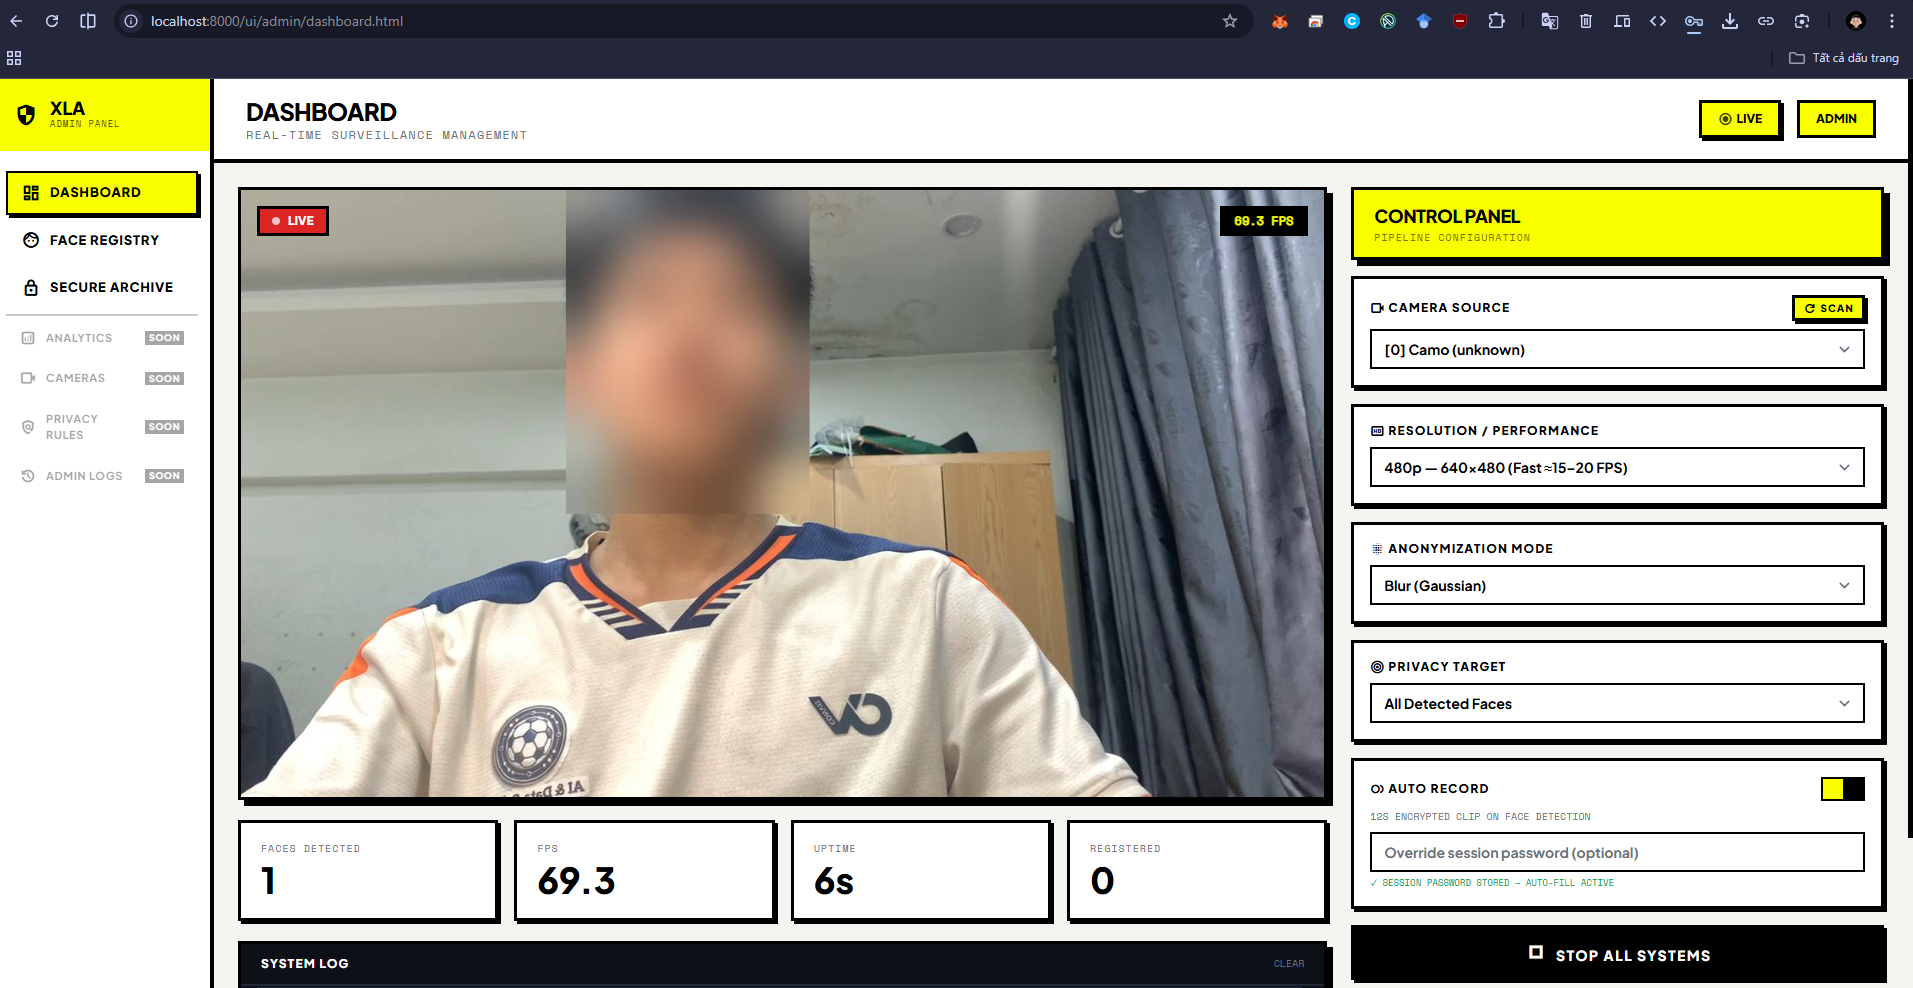
\includegraphics[width=\linewidth]{img/blur.png}\\[2pt]{\small blur}
\end{minipage}\hfill
\begin{minipage}{0.32\textwidth}\centering
  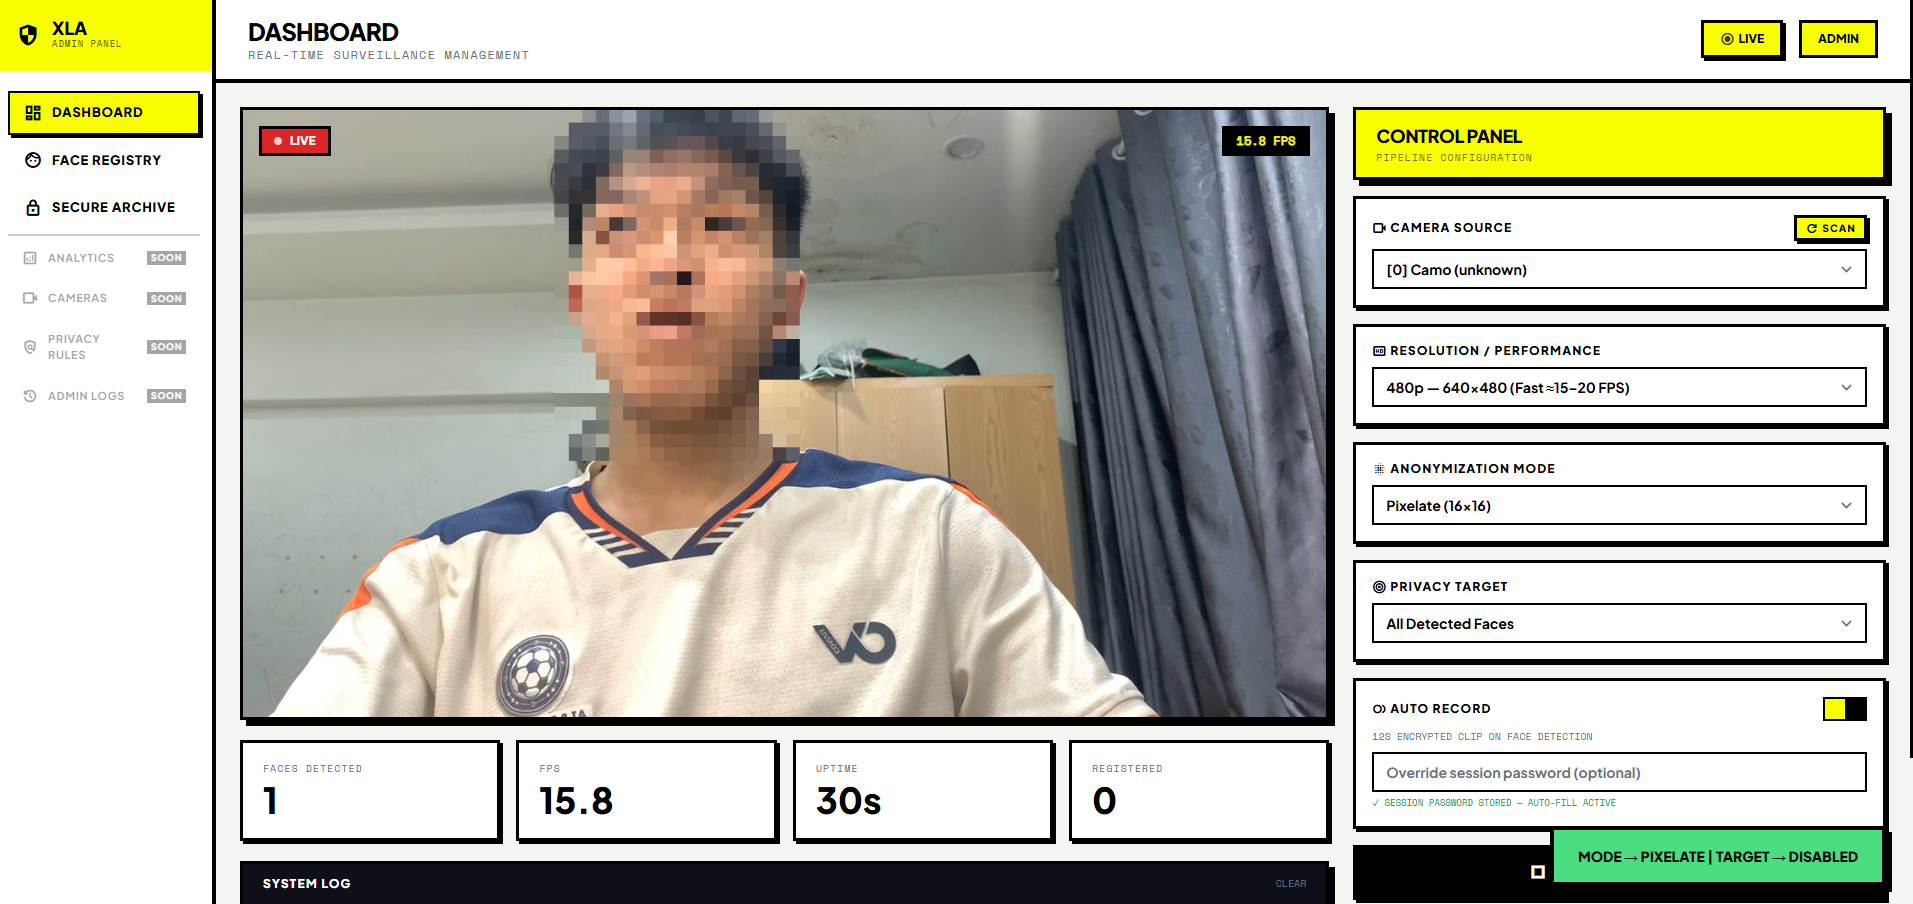
\includegraphics[width=\linewidth]{img/pixelate.png}\\[2pt]{\small pixelate}
\end{minipage}\hfill
\begin{minipage}{0.32\textwidth}\centering
  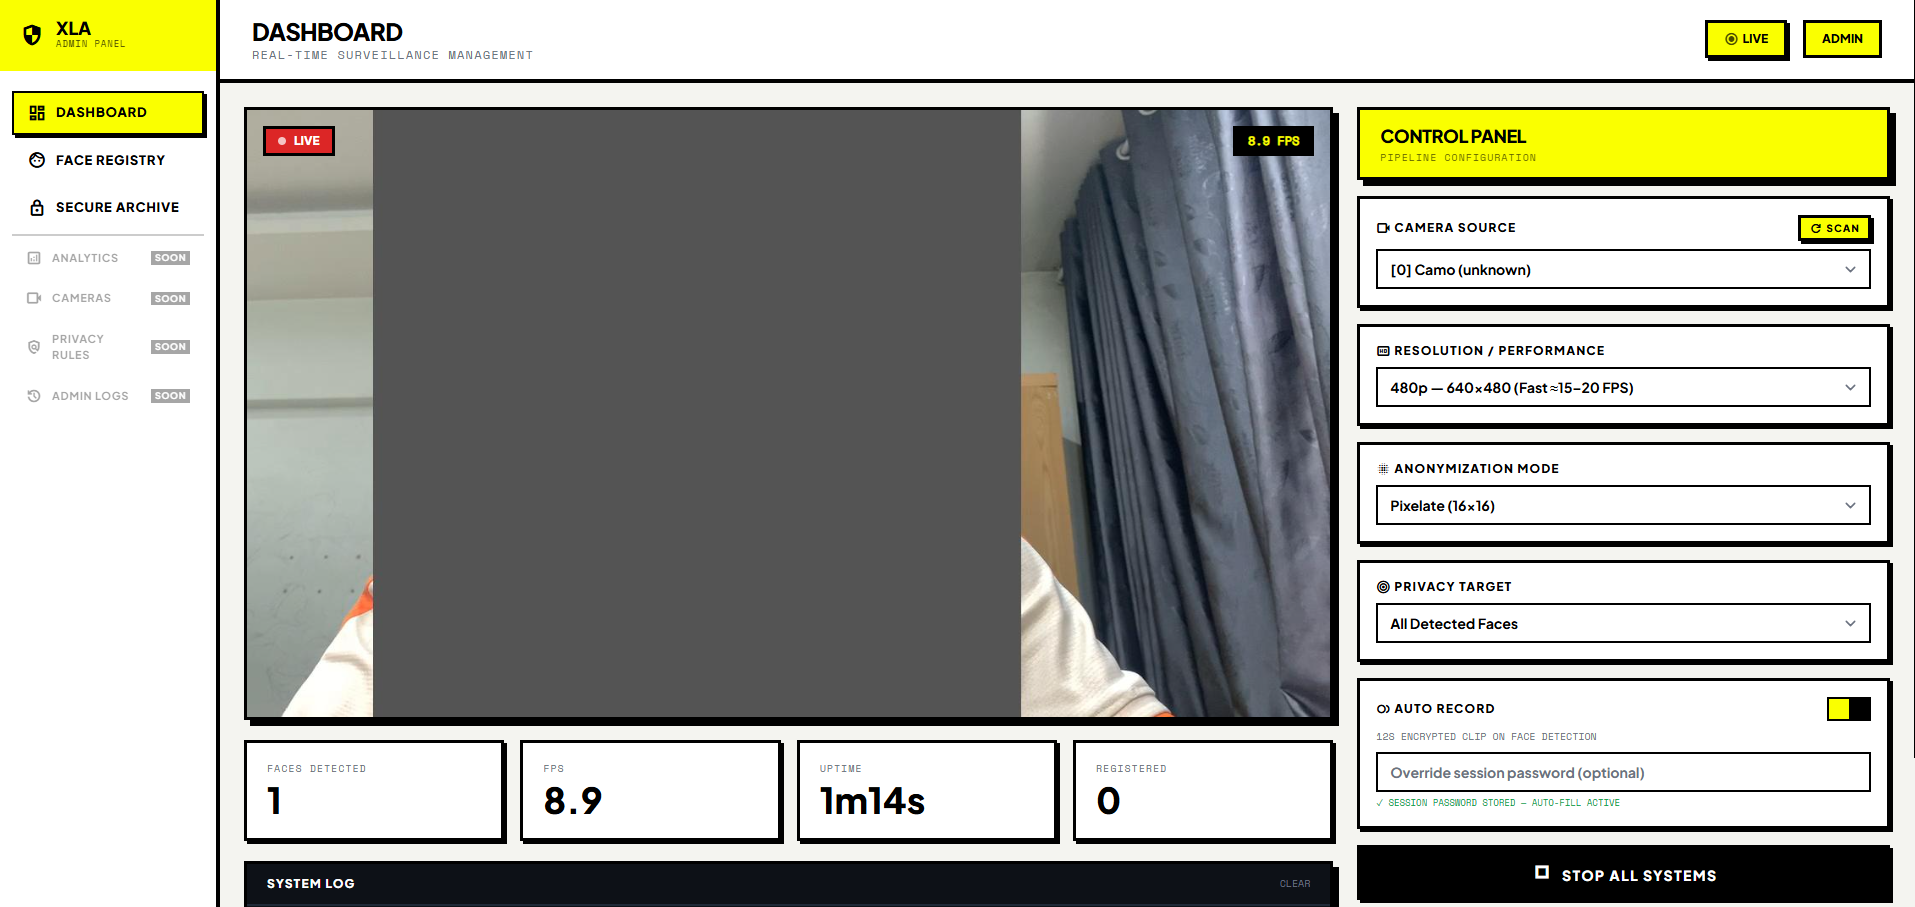
\includegraphics[width=\linewidth]{img/headcloak.png}\\[2pt]{\small headcloak}
\end{minipage}
\\[0.4cm]
\begin{minipage}{0.32\textwidth}\centering
  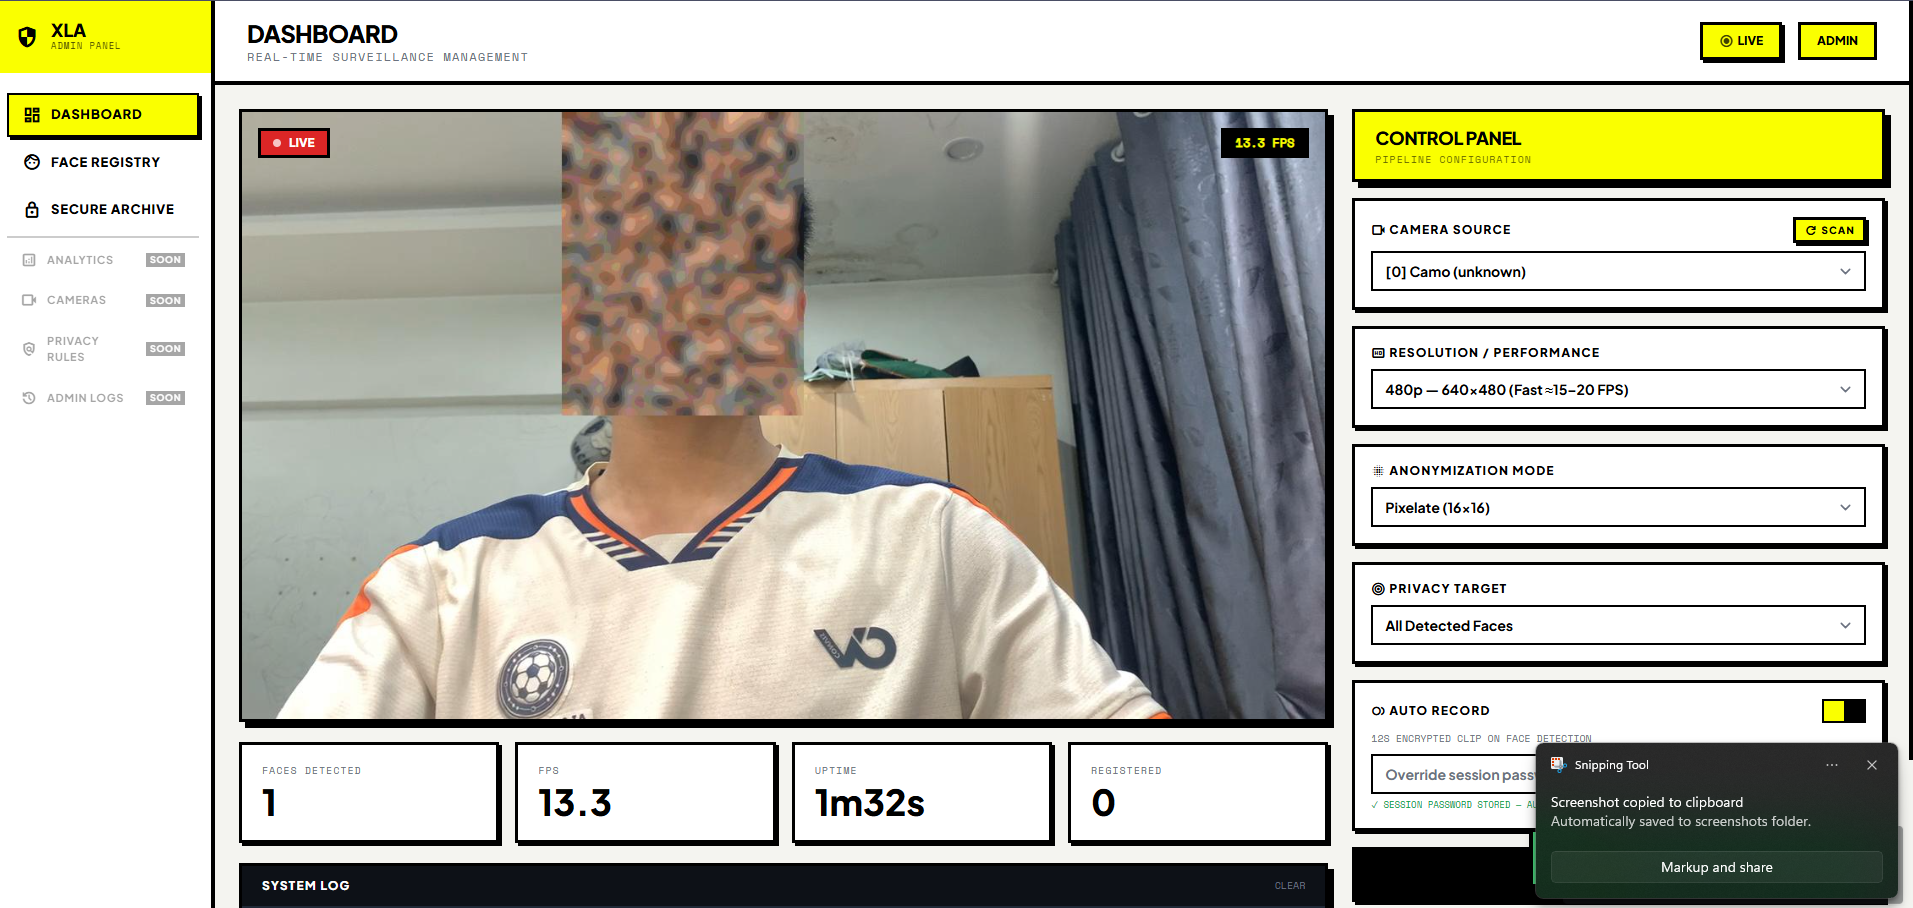
\includegraphics[width=\linewidth]{img/obliterate.png}\\[2pt]{\small obliterate}
\end{minipage}\hfill
\begin{minipage}{0.32\textwidth}\centering
  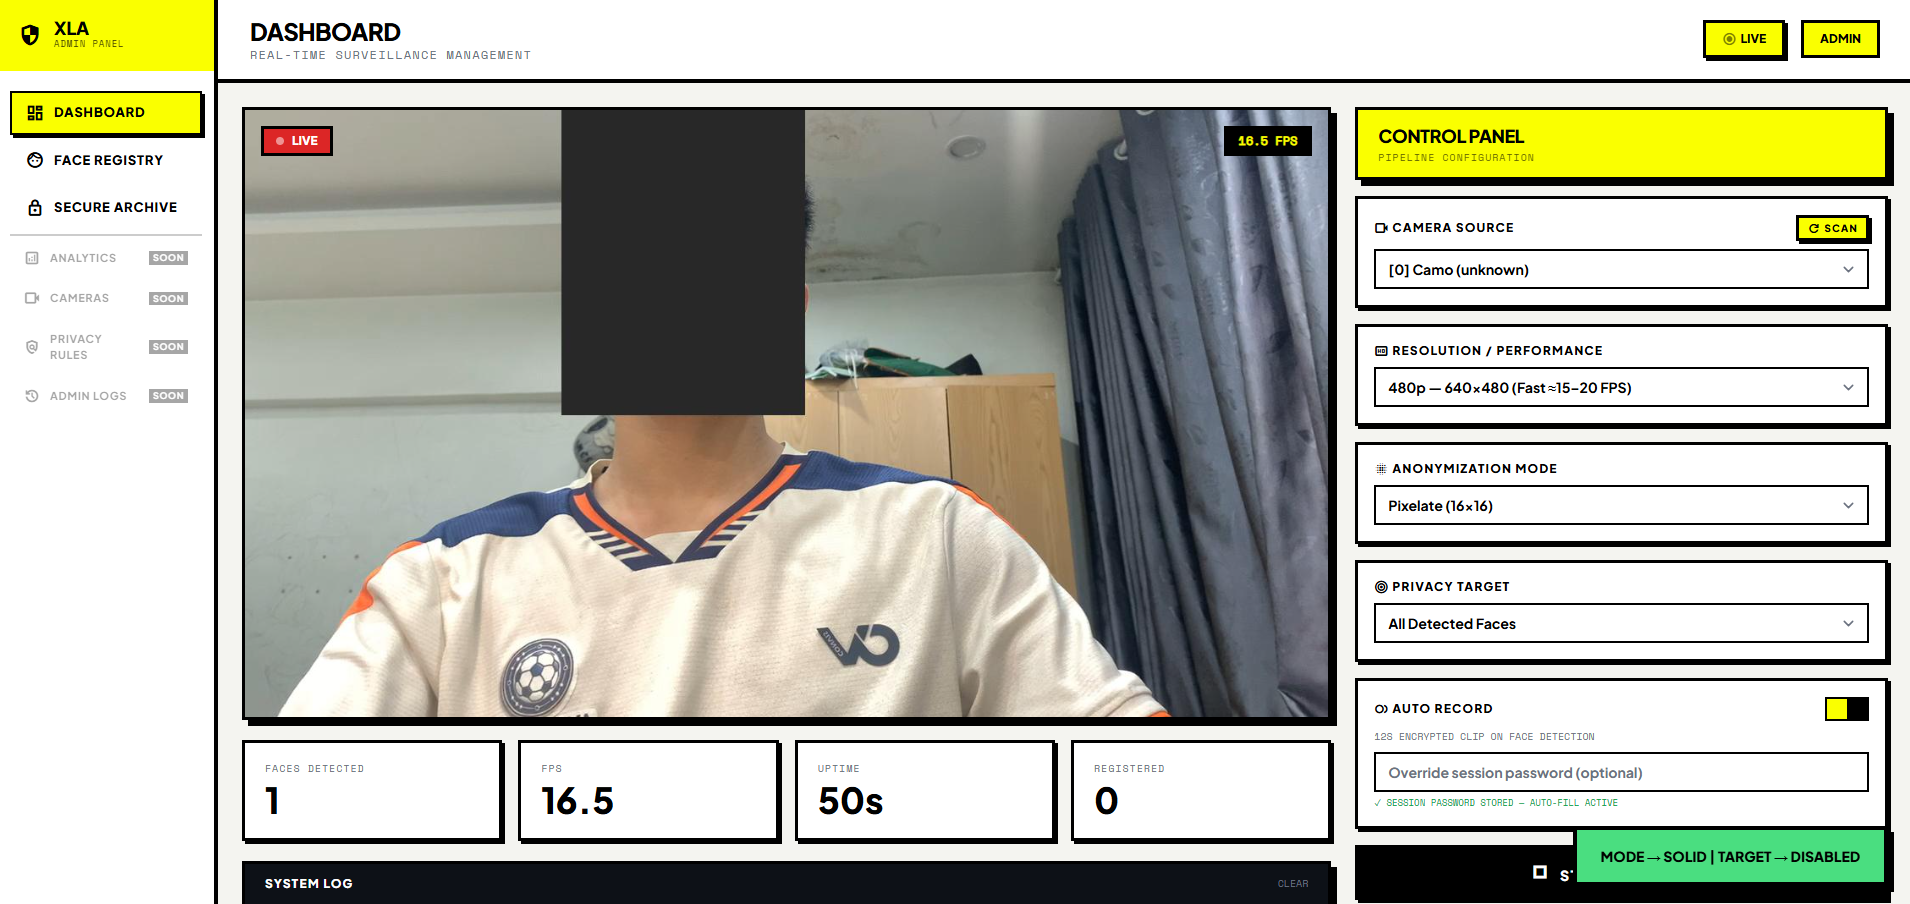
\includegraphics[width=\linewidth]{img/solid.png}\\[2pt]{\small solid}
\end{minipage}\hfill
\begin{minipage}{0.32\textwidth}\centering
  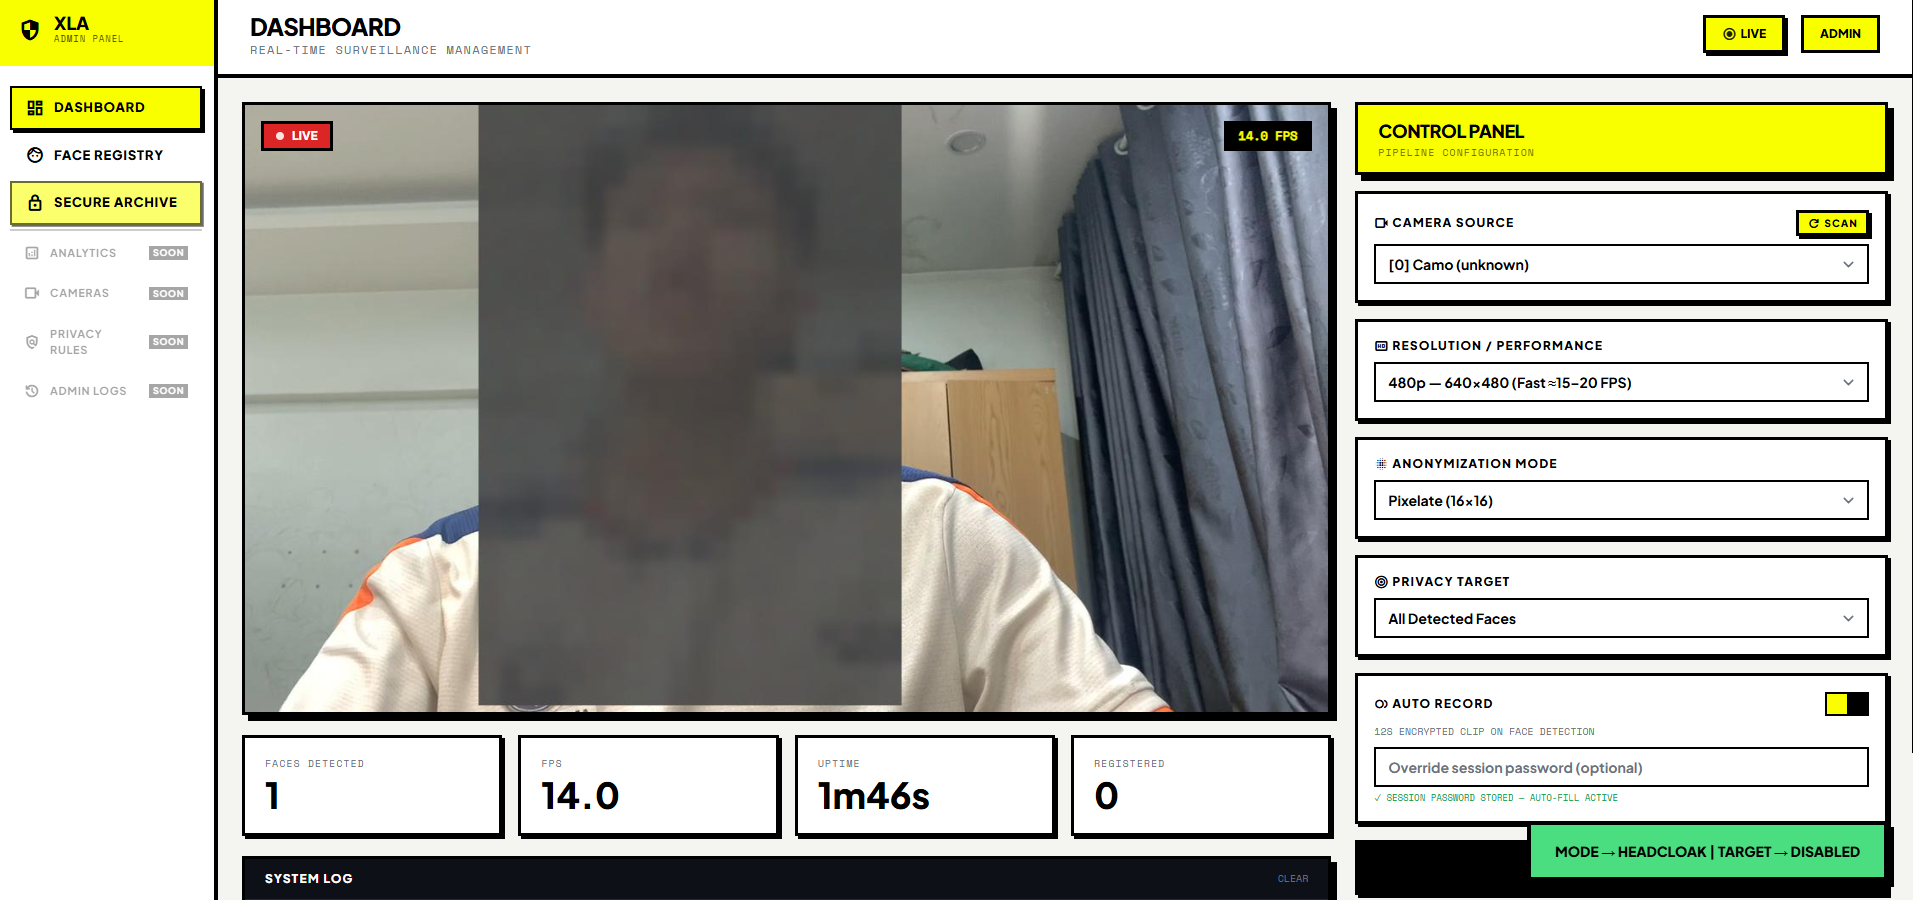
\includegraphics[width=\linewidth]{img/silhouette.png}\\[2pt]{\small silhouette}
\end{minipage}
\caption{So sánh 6 chế độ ẩn danh hoá trên cùng một khung hình thực tế. Từ trái-trên: blur, pixelate, headcloak; dưới: obliterate, solid, silhouette.}
\label{fig:modes_compare}
\end{figure}

\subsubsection{Giao diện web Admin Dashboard}

\begin{figure}[H]
\centering
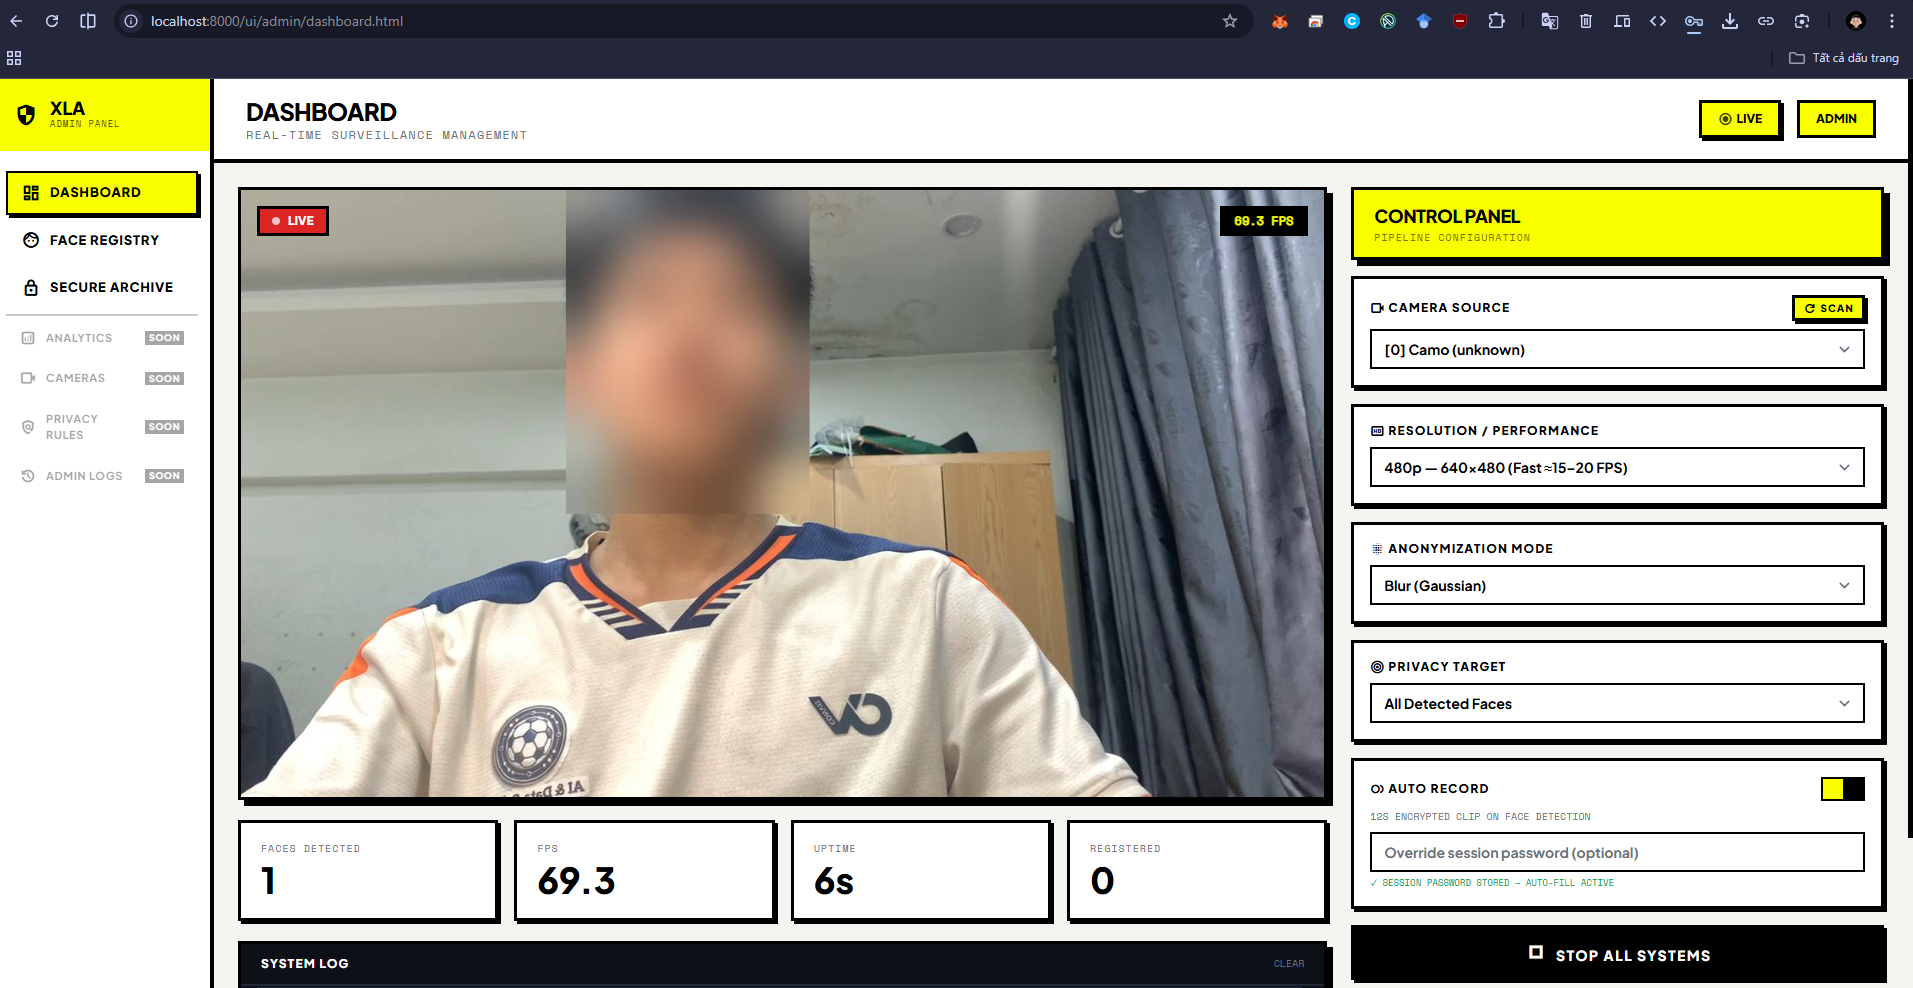
\includegraphics[width=0.95\textwidth]{img/admin_dashboard.png}
\caption{Giao diện Admin Dashboard hiển thị luồng video trực tiếp với chế độ blur đang hoạt động.}
\label{fig:admin_dashboard}
\end{figure}

\subsubsection{Giao diện người dùng --- Live Portal}

\begin{figure}[H]
\centering
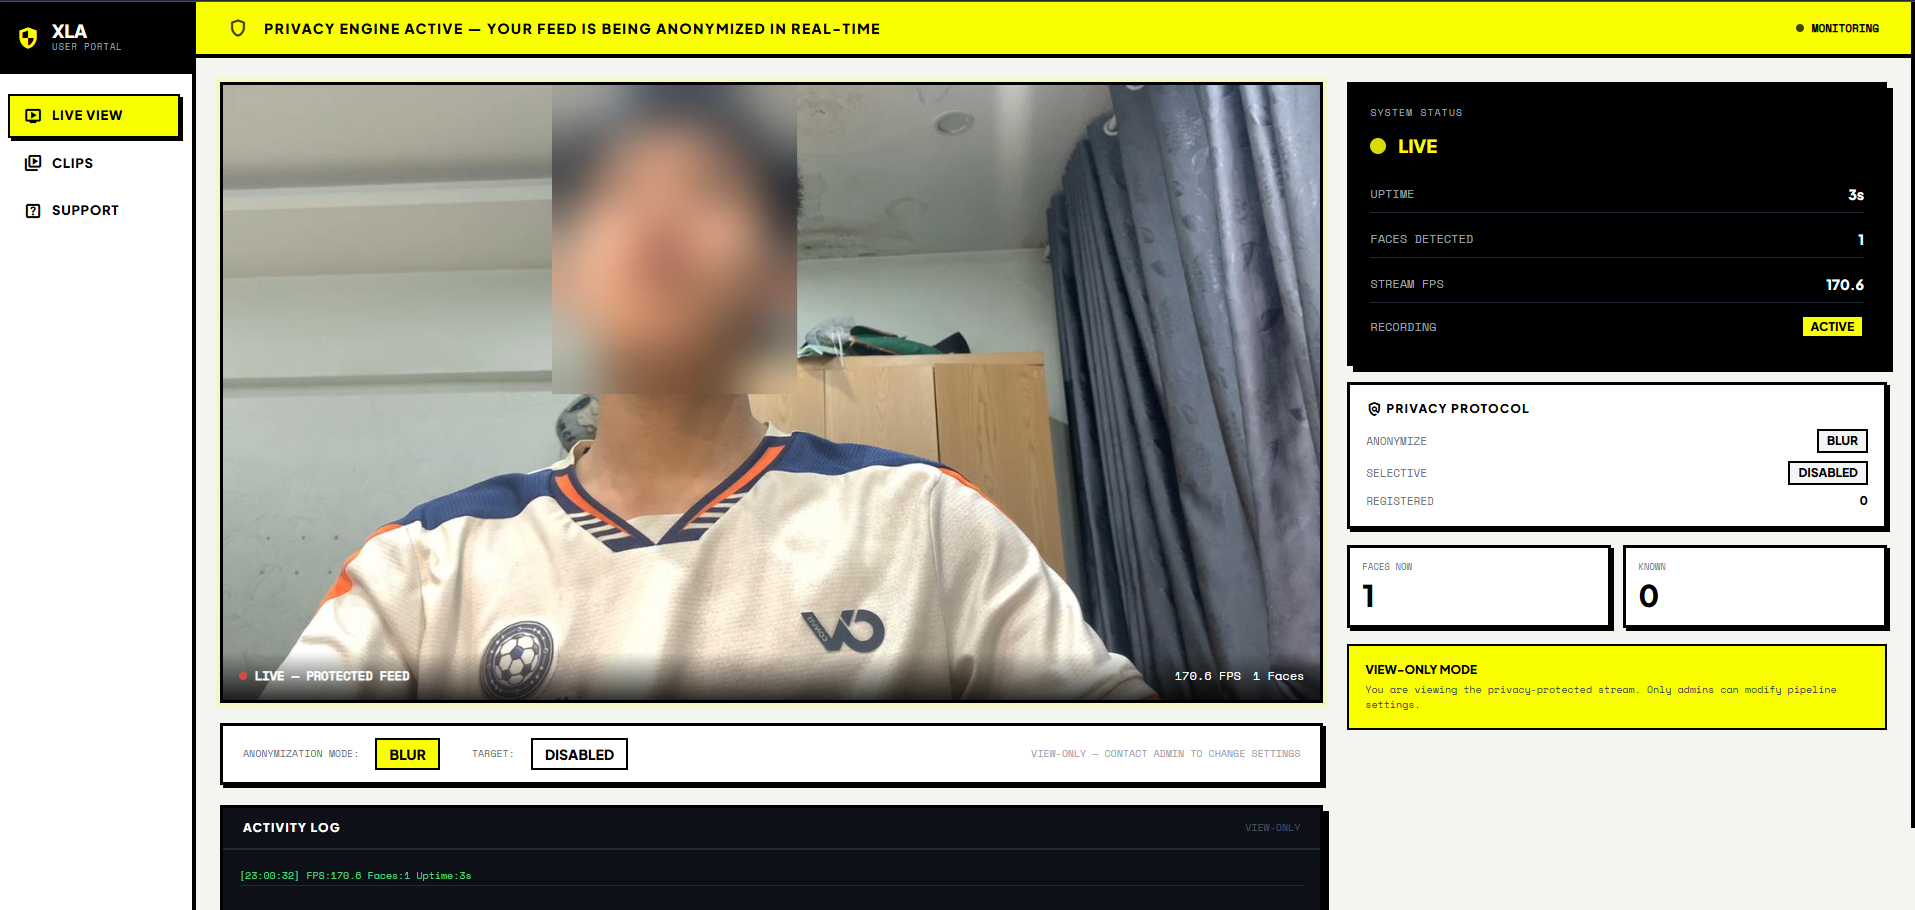
\includegraphics[width=0.95\textwidth]{img/user_portal.png}
\caption{Giao diện User Portal --- Live View. Khuôn mặt đã được ẩn danh hoá, người dùng thường không thể xem bản gốc.}
\label{fig:user_portal}
\end{figure}

\subsubsection{Biểu đồ so sánh FPS theo chế độ}

\begin{figure}[H]
\centering
\begin{tikzpicture}
\begin{scope}[xscale=0.11, yscale=0.06]
% Axes
\draw[->] (0,0) -- (80,0) node[right]{\small FPS};
\draw[->] (0,0) -- (0,55);
% Y labels (mode names)
\foreach \name/\y in {
  {silhouette/strong}/5,
  {silhouette/fast}/12,
  {obliterate/str}/20,
  {blur/strict}/27,
  {blur/balanced}/34,
  {pixelate/bal}/41,
  {pixelate/fast}/49
}{
  \node[right, font=\tiny] at (-2, \y) {\name};
}
% Bars
\fill[red!70]      (0,2) rectangle (15.71,8);
\fill[red!50]      (0,9) rectangle (27.24,15);
\fill[orange!80]   (0,17) rectangle (37.70,23);
\fill[orange!60]   (0,24) rectangle (32.37,30);
\fill[blue!60]     (0,31) rectangle (36.67,37);
\fill[green!60]    (0,38) rectangle (41.12,44);
\fill[green!80]    (0,46) rectangle (72.53,52);
% Value labels
\foreach \val/\y in {15.71/5, 27.24/12, 37.70/20, 32.37/27, 36.67/34, 41.12/41, 72.53/49}{
  \node[font=\tiny, right] at (\val+0.5, \y) {\val};
}
% X axis ticks
\foreach \x in {0,20,40,60,80}{
  \draw (\x, 0) -- (\x, -1);
  \node[below, font=\tiny] at (\x, -1) {\x};
}
\end{scope}
\end{tikzpicture}
\caption{So sánh FPS theo chế độ và preset (CPU-only, 100 frame). Xanh lá = hiệu suất cao, đỏ = thấp. Đường 25 FPS là ngưỡng real-time tối thiểu.}
\label{fig:fps_chart}
\end{figure}

% ============================================================
%  CHƯƠNG 6: KẾT LUẬN
% ============================================================
\section{Kết luận}
\label{sec:ketluan}

\subsection{Tổng kết}
\label{subsec:tongket}

Báo cáo này đã trình bày toàn bộ quá trình thiết kế, triển khai và đánh giá hệ thống \textbf{XLA Face Privacy System} --- một hệ thống camera giám sát thời gian thực đặt quyền riêng tư làm trung tâm. Xuất phát từ bài toán mâu thuẫn giữa quyền riêng tư và nhu cầu bằng chứng trong giám sát hiện đại, đề tài đã đề xuất và hiện thực hóa một giải pháp kỹ thuật toàn diện dựa trên kiến trúc lưu trữ kép.

\medskip
Hệ thống tích hợp thành công các công nghệ tiên tiến:
\begin{itemize}
    \item \textbf{YOLOv11n-face} cho phát hiện khuôn mặt thời gian thực với tốc độ tới 72 FPS trên CPU.
    \item \textbf{InsightFace buffalo\_l} (ArcFace 512D) cho nhận diện thành viên với độ chính xác cao.
    \item \textbf{9 chế độ ẩn danh hoá} đa dạng từ mức độ nhẹ đến mạnh nhất.
    \item \textbf{AES-256-GCM + PBKDF2-SHA256} (390.000 iterations) cho lưu trữ mã hoá chuẩn công nghiệp.
    \item \textbf{FastAPI + 4 giao thức streaming} cho backend hiệu suất cao.
    \item \textbf{Giao diện web đầy đủ} cho cả admin và người dùng thường.
\end{itemize}

\subsection{Đóng góp của đề tài}
\label{subsec:donggop}

Đề tài có các đóng góp chính sau:

\begin{enumerate}[1.]
    \item \textbf{Kiến trúc Privacy-First mới}: Thiết kế hệ thống lưu trữ kép (blurred MP4 + AES-encrypted .enc) với kiến trúc phân quyền rõ ràng: người dùng thường chỉ thấy video đã ẩn danh hoá, admin mới có thể xem bản gốc.
    
    \item \textbf{Đánh giá định lượng toàn diện}: Xây dựng framework đánh giá hai chiều (hiệu suất + bảo mật) với các chỉ số cụ thể (FPS, SSIM, cosine similarity, recognition prevention rate), đưa ra so sánh có căn cứ đo lường giữa 9 chế độ ẩn danh hoá trên 4 preset.
    
    \item \textbf{Phát hiện điểm yếu của pixelate}: Kết quả thực nghiệm cho thấy pixelate \textit{không đủ} bảo vệ quyền riêng tư trước hệ thống nhận diện hiện đại (cosine similarity 0,98 sau pixelate), điều này thường bị bỏ qua trong các hệ thống thực tế.
    
    \item \textbf{Tích hợp bảo mật đúng cách}: Áp dụng đúng các tiêu chuẩn bảo mật thực tiễn: salt ngẫu nhiên riêng từng clip, PBKDF2 với 390.000 iterations (OWASP 2023), Scrypt cho face lock, constant-time comparison, zero plaintext password storage.
    
    \item \textbf{API mở và có thể mở rộng}: REST API đầy đủ 25+ endpoints cho phép tích hợp với hệ thống khác hoặc thay thế frontend bất kỳ lúc nào.
\end{enumerate}

\subsection{Hạn chế và thách thức}
\label{subsec:hanche}

Đề tài còn tồn tại các hạn chế sau đây cần thừa nhận:

\begin{enumerate}[1.]
    \item \textbf{Phụ thuộc vào ánh sáng và góc nhìn}: Detector YOLOv11n-face bỏ sót khuôn mặt ở góc nghiêng $> 45°$, trong tối, hoặc khi bị che khuất một phần. Điều này có thể để lọt khuôn mặt chưa được ẩn danh hoá trong một số khung hình.
    
    \item \textbf{Chỉ một pipeline tại một thời điểm}: Thiết kế singleton pipeline không hỗ trợ xử lý đồng thời nhiều camera. Đây là giới hạn kiến trúc quan trọng cho ứng dụng quy mô lớn.
    
    \item \textbf{Lưu trữ JSON không thể mở rộng}: Sử dụng JSON thuần cho face database không phù hợp khi số thành viên lên đến hàng nghìn. Tốc độ truy vấn sẽ giảm và nguy cơ race condition khi write đồng thời.
    
    \item \textbf{Chưa có xác thực API đầy đủ}: Các endpoint thông thường không yêu cầu token xác thực. Trong production, cần thêm lớp authentication (JWT/OAuth2) cho toàn bộ API.
    
    \item \textbf{Blur không đủ bảo vệ}: Như được chứng minh trong Chương 5, chế độ blur truyền thống không ngăn nhận diện bởi deep learning. Người dùng cần được hướng dẫn chọn chế độ phù hợp.
    
    \item \textbf{Bộ nhớ pre-buffer}: Pre-buffer 3 giây lưu trong RAM. Với camera 4K 60fps, bộ nhớ cần cho pre-buffer có thể lên đến vài GB.
    
    \item \textbf{Chưa đánh giá trên tập dữ liệu chuẩn}: Thực nghiệm được tiến hành trên tập dữ liệu nội bộ nhỏ, chưa có đánh giá trên các benchmark công khai như LFW, CFP-FP, AgeDB.
\end{enumerate}

\subsection{Hướng phát triển tương lai}
\label{subsec:huongphat}

Dựa trên các hạn chế đã xác định, các hướng phát triển sau đây được đề xuất:

\subsubsection{Ngắn hạn (3--6 tháng)}
\begin{itemize}
    \item \textbf{Multi-camera support}: Refactor pipeline từ singleton sang multi-instance, mỗi camera có pipeline riêng, quản lý qua session ID.
    \item \textbf{API authentication}: Thêm JWT-based authentication với role-based access control (RBAC): \texttt{viewer}, \texttt{member}, \texttt{admin}.
    \item \textbf{SQLite cho face database}: Thay JSON bằng SQLite với vector extension cho indexed embedding search.
    \item \textbf{GPU acceleration}: Thêm hỗ trợ CUDA/TensorRT cho môi trường có GPU để tăng FPS thêm 5--10x.
\end{itemize}

\subsubsection{Trung hạn (6--18 tháng)}
\begin{itemize}
    \item \textbf{Deep anonymization}: Tích hợp các kỹ thuật generative model (GAN-based face de-identification) như DeepPrivacy \cite{hasler2019deepprivacy} để tạo khuôn mặt giả thực sự thay thế, vừa bảo vệ quyền riêng tư vừa giữ ngữ cảnh tự nhiên hơn.
    \item \textbf{Edge deployment}: Tối ưu hóa model với quantization (INT8) để triển khai trên thiết bị nhúng (Raspberry Pi, Jetson Nano) hoặc camera thông minh.
    \item \textbf{Federated privacy-preserving recognition}: Nhận diện thành viên mà không cần gửi ảnh gốc về server --- dùng on-device inference và chỉ truyền kết quả nhị phân (nhận ra/không nhận ra).
    \item \textbf{Audit log mã hoá}: Ghi log tất cả truy cập giải mã clip với timestamp, đảm bảo trách nhiệm giải trình (accountability) ngay cả khi admin truy cập bản gốc.
\end{itemize}

\subsubsection{Dài hạn (nghiên cứu)}
\begin{itemize}
    \item \textbf{Differential Privacy cho embedding}: Thêm nhiễu Gaussian đã hiệu chỉnh vào embedding trước khi lưu, đảm bảo bảo mật toán học (differential privacy) ngay cả khi database bị lộ.
    \item \textbf{Tuân thủ GDPR đầy đủ}: Cài đặt \textit{right to be forgotten} (xóa hoàn toàn mọi dấu vết của một cá nhân), \textit{data minimization} (tự động xóa clip sau $N$ ngày), và \textit{consent management}.
    \item \textbf{Zero-knowledge decryption}: Nghiên cứu cơ chế cho phép admin xác nhận danh tính mà không bao giờ giao khoá trực tiếp cho server, dùng zero-knowledge proof.
\end{itemize}

% =========================================================
\subsection{Điểm sáng sáng tạo (Creative Spark)}
\label{subsec:creativespark}
% =========================================================

Phần này nêu bật những điểm sáng kỹ thuật và tư duy thiết kế mà nhóm đóng góp vượt ra ngoài yêu cầu bài tập thông thường, phù hợp với Tiêu chí 4.1 của rubric đánh giá.

\subsubsection{Điểm sáng 1: Kiến trúc lưu trữ kép (Dual-Layer Storage)}

Thay vì chọn một trong hai cực (lưu thô hoặc không lưu), nhóm thiết kế kiến trúc \textbf{lưu đồng thời hai bản}: (1) clip đã ẩn danh hoá hoàn toàn dưới dạng MP4 thường cho xem ngay lập tức, và (2) bản gốc mã hoá AES-256-GCM dưới dạng file .enc chỉ admin với mật khẩu đúng mới giải mã được. Đây là cách tiếp cận vừa \textit{bảo vệ quyền riêng tư theo mặc định} vừa \textit{bảo tồn bằng chứng pháp lý}. Kiến trúc này là sự cân bằng kỹ thuật tinh tế giữa hai nguyên tắc đối lập.

\subsubsection{Điểm sáng 2: Phát hiện điểm yếu bảo mật của Pixelate}

Kết quả thực nghiệm (Chương 5) cho thấy pixelate với \textit{bất kỳ} block size nào đều \textbf{không ngăn được nhận diện bằng deep learning} (cosine similarity $\geq 0.48$ ngay cả với block size 256). Đây là phát hiện quan trọng về mặt thực tiễn:
\begin{itemize}
    \item Nhiều hệ thống giám sát thương mại hiện tại dùng pixelate và tuyên bố ẩn danh hoá, nhưng thực tế không bảo vệ.
    \item Phát hiện này có giá trị ứng dụng thực tế: hướng dẫn người dùng chọn headcloak hoặc silhouette thay vì pixelate khi cần bảo vệ danh tính mạnh.
\end{itemize}

\subsubsection{Điểm sáng 3: CPU-Only Real-Time Processing}

Toàn bộ pipeline chạy trên CPU với tốc độ 72 FPS (pixelate/fast). Điều này đạt được qua 4 tầng tối ưu:
\begin{enumerate}[a)]
    \item Vectorization NumPy/BLAS thay Python loops (145× speedup cho 100 thành viên).
    \item Skip detection mỗi $N$ frame (35\% FPS gain).
    \item Downsample-blur-upsample (20× speedup vs. blur kích thước gốc).
    \item Drop-frame queue + async architecture tránh blocking.
\end{enumerate}
Đây không phải tối ưu ``viết lại code nhanh hơn'', mà là tối ưu có tính toán thuật toán với phép đo thực nghiệm trước/sau.

\subsubsection{Điểm sáng 4: Mã hoá bảo mật đúng cách (Security Best Practices)}

Thay vì dùng mã hoá đơn giản hoặc mật khẩu plaintext, hệ thống áp dụng đúng các tiêu chuẩn:
\begin{itemize}
    \item \textbf{Không bao giờ lưu mật khẩu plaintext}: Dùng Scrypt hash cho face lock, PBKDF2 KDF cho encryption key.
    \item \textbf{Salt ngẫu nhiên riêng từng clip}: Ngăn rainbow table và identical-ciphertext attacks.
    \item \textbf{AES-256-GCM}: Vừa mã hoá vừa xác thực toàn vẹn --- phát hiện ngay nếu file bị tampering.
    \item \textbf{PBKDF2 390.000 iterations}: Brute-force time ước tính 12 năm với phần cứng hiện tại.
    \item \textbf{Constant-time comparison}: Tránh timing attack khi so sánh hash.
\end{itemize}

\subsubsection{Điểm sáng 5: Hệ thống 9 chế độ với đánh giá định lượng}

Thay vì chỉ cài đặt ``blur khuôn mặt'', nhóm thiết kế \textbf{9 chế độ ẩn danh hoá} với đánh giá định lượng bảo mật. Kết quả tạo ra \textbf{ma trận đánh giá 2 chiều} (privacy strength $\times$ performance) cung cấp thông tin để người dùng lựa chọn dựa trên tradeoff rõ ràng, không phải dựa trên cảm quan.

\medskip

% =========================================================
\subsection{Tóm tắt quy trình khoa học}
\label{subsec:quytrinhkhoa}
% =========================================================

Để đảm bảo tính khoa học, nhóm tuân thủ quy trình nghiên cứu có cấu trúc rõ ràng:

\begin{enumerate}[label=\textbf{Bước \arabic*.}]
    \item \textbf{Xác định vấn đề} $\rightarrow$ Mâu thuẫn privacy vs. evidence trong camera giám sát. Formal definition: cần hệ thống $\mathcal{S}$ sao cho $\text{Privacy}(\mathcal{S}) \geq \tau_{priv}$ đồng thời $\text{Evidence}(\mathcal{S}) = 1$.
    
    \item \textbf{Đặt câu hỏi nghiên cứu} $\rightarrow$ (i) Chế độ nào đủ bảo vệ quyền riêng tư trước deep learning? (ii) Chi phí hiệu suất của từng chế độ là bao nhiêu? (iii) Có thể đạt real-time CPU-only không?
    
    \item \textbf{Xây dựng giả thuyết} $\rightarrow$ H1: Pixelate không đủ bảo vệ. H2: Headcloak/silhouette ngăn nhận diện hoàn toàn. H3: Tốc độ $\geq 25$ FPS (real-time) là khả thi trên CPU.
    
    \item \textbf{Thiết kế thực nghiệm} $\rightarrow$ 9 chế độ $\times$ 4 preset, mỗi tổ hợp chạy 100 frame, đo 5 chỉ số (FPS, SSIM, PSNR, cosine similarity, tỷ lệ ngăn nhận diện).
    
    \item \textbf{Thu thập dữ liệu} $\rightarrow$ Kết quả lưu vào \texttt{bench\allowbreak{}mark\_results.csv} và \texttt{se\allowbreak{}cu\allowbreak{}rity\_eva\allowbreak{}lu\allowbreak{}ation.csv}.
    
    \item \textbf{Phân tích kết quả} $\rightarrow$ H1 xác nhận (pixelate sim $=0.98$). H2 xác nhận (headcloak, silhouette, obliterate ngăn $100\%$). H3 xác nhận (pixelate/fast: 72 FPS).
    
    \item \textbf{Rút ra kết luận} $\rightarrow$ Không phải mọi ``ẩn danh hoá'' đều như nhau; cần phân biệt visual anonymization (bảo vệ trước mắt người) và algorithmic anonymization (bảo vệ trước AI).
\end{enumerate}

\medskip

% =========================================================
\subsection{Kết luận chung}
\label{subsec:ketluanchung}

Đề tài đã đạt được mục tiêu đặt ra: xây dựng thành công hệ thống camera giám sát privacy-first hoàn chỉnh, từ camera input đến web interface, với triết lý \textit{ẩn danh hoá theo mặc định -- bằng chứng theo yêu cầu}. Kết quả thực nghiệm định lượng cung cấp cơ sở rõ ràng để người dùng lựa chọn chế độ phù hợp cho từng ngữ cảnh, đồng thời phát hiện được điểm yếu quan trọng của pixelate --- thông tin có giá trị thực tiễn cho các nhà phát triển hệ thống camera tương tự.

\medskip
Trong bối cảnh quyền riêng tư ngày càng trở thành quyền cơ bản được pháp lý bảo vệ, các hệ thống như XLA Face Privacy System không chỉ là giải pháp kỹ thuật mà còn là hiện thực hóa của một triết lý: \textbf{công nghệ phải phục vụ con người, không phải theo dõi con người}.

\medskip


% ════════════════════════════════════════════════════════════════════════════
%   TÀI LIỆU THAM KHẢO
% ════════════════════════════════════════════════════════════════════════════
\newpage
\renewcommand{\refname}{Tài liệu tham khảo}
\addcontentsline{toc}{section}{Tài liệu tham khảo}
\bibliographystyle{plain}
\bibliography{ref_xla}

\end{document}
